\documentclass[11pt,a4paper,twoside,openright]{report}

\usepackage[pdftex]{graphicx} % Biblioteca para uso de figuras
\usepackage{subcaption}
\usepackage{color}

\usepackage[brazil]{babel} % Biblioteca para uso da l�ngua portuguesa
\usepackage[T1]{fontenc} % Biblioteca para uso da acentua��o de entrada
\usepackage[latin1]{inputenc} % Biblioteca para uso da acentua��o de sa�da
\usepackage{enumitem} % biblioteca para formatar listas, enumeradas ou n�o
\setlist[itemize]{itemsep=-1ex}

\usepackage{hyperref}
\hypersetup{
    colorlinks,
    citecolor=black,
    filecolor=black,
    linkcolor=black,
    urlcolor=black
}

\usepackage{array} % biblioteca para ajustar tamanho das colunas de tabela
\newcolumntype{P}[1]{>{\centering\let\newline\\\arraybackslash\hspace{0pt}}p{#1}}
\newcolumntype{M}[1]{>{\centering\let\newline\\\arraybackslash}m{#1}}
\usepackage{longtable}%para quebrar a tabela em multiplas paginas

%\usepackage{pbox} %pacote pra poder quebrar linha dentro de c�lulas da tabela

\usepackage{siunitx} % biblioteca para uso de unidades si
\usepackage{amsthm,amsfonts,amsmath,amssymb}  % Biblioteca para uso de comandos matem�ticos
\usepackage{pslatex}
\usepackage{pstricks,pst-node,color,pst-gantt,pst-coil}
\usepackage{scalefnt}
\usepackage{float} %Permite colocar "\begin{figure}[H]" e colocar imagem exatamente onde desejar
\usepackage[hyphens]{url} % Para Aceitar URL nas referencias
\usepackage{pdfpages}
\usepackage{caption,setspace}

\usepackage{eurosym} %Pacote para possibilitar o uso do s�mbolo de euro "\euro"

\usepackage{listings} % para importa��o de c�digos fonte 
\renewcommand{\lstlistingname}{C�digo-fonte}
\renewcommand*{\lstlistlistingname}{Lista de C�digos-fonte}
%%%%%%%%%%%%%%% Configura��o da formata��o das linguagens %%%%%%%%%%%%%%%%%%%
% Definindo novas cores
\definecolor{verde}{rgb}{0,0.5,0}
% Configurando layout para mostrar codigos Bash
\lstset{
	tabsize=2,
	language=bash,
	basicstyle=\ttfamily\small, 
	keywordstyle=\color{blue}, 
	stringstyle=\color{verde}, 
	commentstyle=\color{red}, 
	extendedchars=true, 
	showspaces=false, 
	showstringspaces=false, 
	numbers=left,
	numberstyle=\tiny,
	breaklines=true, 
	%backgroundcolor=\color{green!10},
	breakautoindent=true, 
	captionpos=b,
	xleftmargin=0pt,
}
%%%%%%%%%%%%% Layout para Device Tree %%%%%%%%%%%%%%%%%%%%%%%%
\lstdefinelanguage{dtc}{
	%keywords={typeof, new, true, false, catch, function, return, null, catch, switch, var, if, in, while, do, else, case, break},
	%keywordstyle=\color{blue}\bfseries,
	%ndkeywords={class, export, boolean, throw, implements, import, this},
	%ndkeywordstyle=\color{darkgray}\bfseries,
	identifierstyle=\color{black},
	sensitive=false,
	comment=[l]{//},
	morecomment=[s]{/*}{*/},
	commentstyle=\color{purple}\ttfamily,
	stringstyle=\color{red}\ttfamily,
	morestring=[b]',
	morestring=[b]"
}
%%%%%%%%%%%%% Fim Layout para Device Tree %%%%%%%%%%%%%%%%%%%%%%%%

%%%%%%%%%%%%% Layout para Javascript %%%%%%%%%%%%%%%%%%%%%%%%
\definecolor{purple}{rgb}{0.65, 0.12, 0.82}
\lstdefinelanguage{javascript}{
  keywords={break, case, catch, continue, debugger, default, delete, do, else, false, finally, for, function, if, in, instanceof, new, null, return, switch, this, throw, true, try, typeof, var, void, while, with},
  morecomment=[l]{//},
  morecomment=[s]{/*}{*/},
  morestring=[b]',
  morestring=[b]",
  ndkeywords={class, export, boolean, throw, implements, import, this},
  keywordstyle=\color{blue}\bfseries,
  ndkeywordstyle=\color{darkgray}\bfseries,
  identifierstyle=\color{black},
  commentstyle=\color{purple}\ttfamily,
  stringstyle=\color{red}\ttfamily,
  sensitive=true
}
\lstset{
   language=javascript,
   %backgroundcolor=\color{lightgray},
   extendedchars=true,
   basicstyle=\footnotesize\ttfamily,
   showstringspaces=false,
   showspaces=false,
   numbers=left,
   numberstyle=\footnotesize,
   numbersep=9pt,
   tabsize=2,
   breaklines=true,
   showtabs=false,
   captionpos=b
}
%%%%%%%%%%%%% Fim Layout para Javascript %%%%%%%%%%%%%%%%%%%%%%%%


\usepackage{comment}
\usepackage[margin=2.7cm]{geometry}
\renewcommand{\baselinestretch}{1.5}

\setlength{\parskip}{0em}

% Pacote para configurar cabe�alho e rodape
\usepackage{fancyhdr}
\pagestyle{empty}
\fancyhf{} % clear all header and footer fields

\fancypagestyle{plain}{\pagestyle{fancy}}
\renewcommand{\headrulewidth}{0pt}
\renewcommand{\footrulewidth}{0pt}

%Pacote para organizar apendices 
\usepackage[titletoc]{appendix}

%%%%%%%%%%%%%%%%%%%%%%%%%%%%%%%%%%%%%% CONFIGURA��ES DE ANEXOS %%%%%%%%%%%%%%%%%%%%%%%%%%%%%%%%%%%%%%

\newcommand{\annexname}{Anexo}
\makeatletter
\newcommand\annex{\par
  \setcounter{chapter}{0}%
  \setcounter{section}{0}%
  \gdef\@chapapp{\annexname}%
  \gdef\thechapter{\@Roman\c@chapter}}
\makeatother

\newenvironment{poliabstract}[1]
  {\renewcommand{\abstractname}{#1}\begin{abstract}}
  {\end{abstract}}

%%%%%%%%%%%%%%%%%%%%%%%%%%%%%%%%%%%%%% CONFIGURA��ES DE P�GINA %%%%%%%%%%%%%%%%%%%%%%%%%%%%%%%%%%%%%%
%\topmargin -2.1cm
%\oddsidemargin 0.5cm 
%\evensidemargin 0.5cm 
%\textwidth 15cm
%\textheight 25.1cm
	
%%%%%%%%%%%%%%%%%%%%%%%%%%%%%%%%%%%%%%%% IN�CIO DO DOCUMENTO %%%%%%%%%%%%%%%%%%%%%%%%%%%%%%%%%%%%%%%%
\begin{document}
	
%%%%%%%%%%%%%%%%%%%%%%%%%%%%%%%%%%%%%%  INCLUDES %%%%%%%%%%%%%%%%%%%%%%%%%%%%%%%%%%%%%%

%%%%%%%%%%%%%%%%%%%%%%%%%%%%%%%%%%%%%% ELEMENTOS PR�-TEXTUAIS %%%%%%%%%%%%%%%%%%%%%%%%%%%%%%%%%%%%%%
%%%%%%%%%%%%%%%%%%%%%%%%%%%%%%%%%%%%%%% CONFIGURA??ES DE CAPA %%%%%%%%%%%%%%%%%%%%%%%%%%%%%%%%%%%%%%%
\begin{titlepage}
	
	% CAPA PRINCIPAL
	\begin{center}
		\Huge{UNIVERSIDADE DE S�O PAULO}\\
		\vspace{0.02\textheight}
		\huge{ESCOLA DE ENGENHARIA DE S�O CARLOS}\\
		\vspace{0.01\textheight}
		\huge{DEPARTAMENTO DE ENGENHARIA EL�TRICA E DE COMPUTA��O}\\
		\vspace{0.2\textheight}
		\huge{\textbf{Sistema Automatizado de Produ��o de Cerveja, Monitorado e Controlado Remotamente}}
		\vspace{0.2\textheight}
	\end{center}
		
		\large
		{
			\begin{flushleft}
			\Large{ \textbf{Autor}: \hspace{1.45cm} Leonardo Graboski Veiga }\\
			\Large{ \textbf{Orientador}: \hspace{0.3cm} Prof. Dr. Evandro Luis Linhari Rodrigues }\\
			\end{flushleft}
	
			\begin{center}
				\vspace{0.09\textheight}
				\Large{S�o Carlos}\\
				\Large{2015}
			\end{center}
		}
	
\end{titlepage}


%%%%%%%%%%%%%%%%%%%%%%%%%%%%%%%%%%%%%%%%%%%%%%% INSER??O P?GINA EM BRANCO %%%%%%%%%%%%%%%%%%%%%%%%%%%%%%%%%%%%%%%%%%%%%%
\cleardoublepage

%%%%%%%%%%%%%%%%%%%%%%%%%%%%%%%%%%%%%%% FOLHA DE ROSTO %%%%%%%%%%%%%%%%%%%%%%%%%%%%%%%%%%%%%%%
%\vspace{0.01\textheight} 
	\begin{center}
	\vspace{-0.06\textheight}
	%\thispagestyle{empty}
		\Large{\textbf{Leonardo Graboski Veiga}}\\
		\vspace{0.15\textheight}
		\Huge{\textbf{Sistema Automatizado de Produ��o de Cerveja, Monitorado e Controlado Remotamente}} 
		\vspace{0.08\textheight}
	\end{center}
		
		\large
		{
			\begin{flushright}
			\Large{Trabalho de Conclus�o de Curso apresentado} \hspace{1cm}\\
			\Large{� Escola de Engenharia de S�o Carlos, da}\\
			\Large{Universidade de S�o Paulo}\\
			\vspace{0.05\textheight}
			\Large{Curso de Engenharia El�trica}\\
			\vspace{0.05\textheight}
			\Large{ORIENTADOR: Prof. Dr. Evandro Luis Linhari Rodrigues}\\
			\end{flushright}
	
			\begin{center}
				\vspace{0.15\textheight}
				\Large{S�o Carlos}\\
				\Large{2015}
			\end{center}
		}



%%%%%%%%%%%%%%%%%%%%%%%%%%%%%%%%%%%%%%%%%%%%%%% FICHA CATALOGRAFICA % % % % % % % % % % % % % % % % % % %
\newpage

P�gina com a ficha catalogr�fica (em p�gina par).

%ficha catalografica no verso
%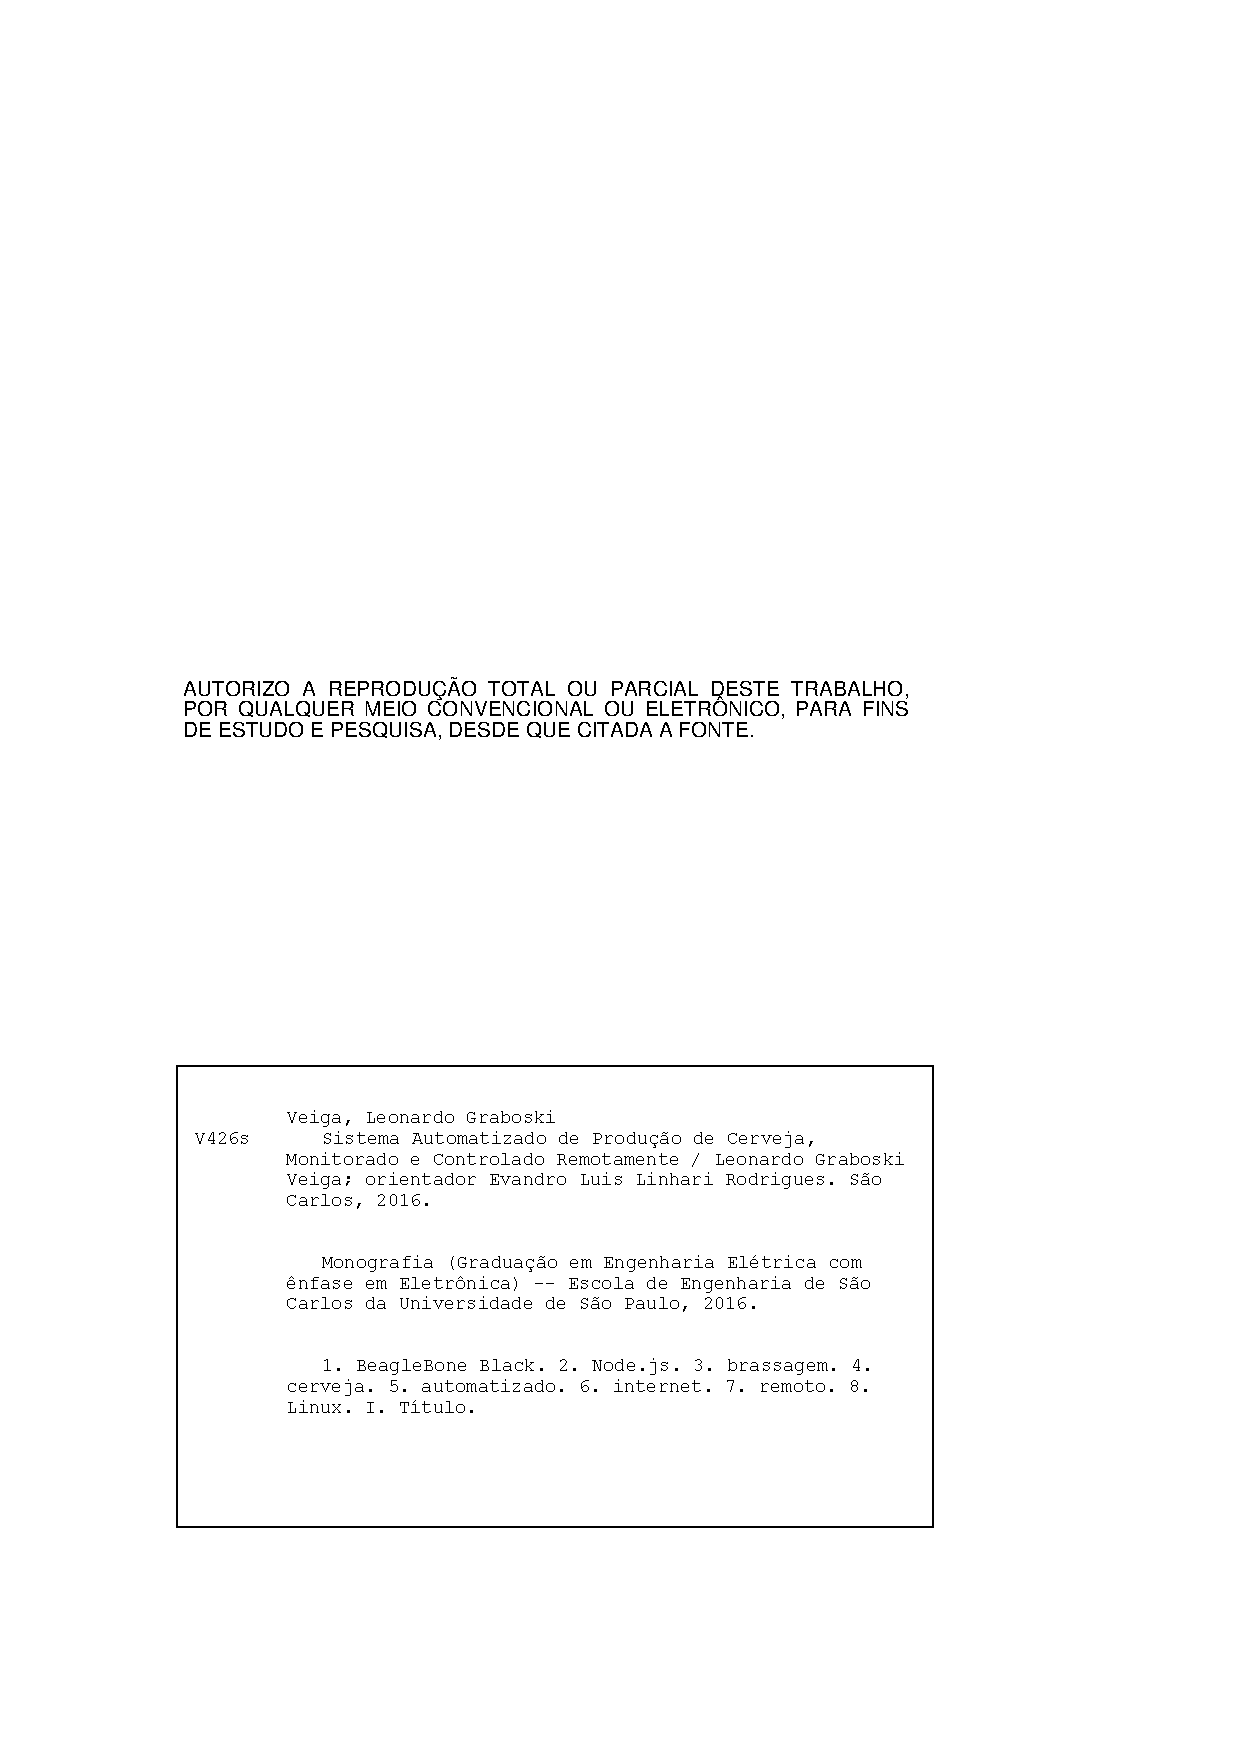
\includepdf{./Resources/ficha_catalografica.pdf}

% % % % % % % % % % % % % % % % % % % % % % % % Folha de aprova��o % % % % % % % % % % % % % % % % % % %
\newpage

p�gina com a folha de aprova��o (p�gina �mpar). \cleardoublepage

\begin{comment}
\begin{figure}[H]
	\centering
	\includegraphics[scale=0.3]{./Resources/aprovacao.jpg}
	\caption{Fluxo de comunica��o entre os principais componentes.}
	\label{Aprovacao}
\end{figure}
\cleardoublepage
\end{comment}

%%%%%%%%%%%%%%%%%%%%%%%%%%%%%%%%%%%%%%%%%%%%%%% DEDICAT?RIA %%%%%%%%%%%%%%%%%%%%%%%%%%%%%%%%%%%%%%%%%%%%%%
\
\vspace{0.11\textheight} 
\begin{center}
\textbf{\Huge{Dedicat�ria}}
\end{center}
\vspace{0.05\textheight}	
		
Dedico este trabalho aos meus pais.
		
\begin{flushright}
Leonardo Graboski Veiga.
\end{flushright}

%%%%%%%%%%%%%%%%%%%%%%%%%%%%%%%%%%%%%%%%%%%%%%% INSER??O P?GINA EM BRANCO %%%%%%%%%%%%%%%%%%%%%%%%%%%%%%%%%%%%%%%%%%%%%%
\cleardoublepage

%%%%%%%%%%%%%%%%%%%%%%%%%%%%%%%%%%%%%%%%%%%%%%% AGRADECIMENTOS %%%%%%%%%%%%%%%%%%%%%%%%%%%%%%%%%%%%%%%%%%%%%%
\
\vspace{0.11\textheight} 

\begin{center}
\textbf{\Huge{Agradecimentos}}
\end{center}

\vspace{0.05\textheight}
			
Tenho convic��o de que quem somos pode ser sintetizado pela soma das intera��es sociais que acumulamos com o passar dos anos. � por isso que agrade�o a todos que passaram por minha vida --- cada um de voc�s � parte daquilo que hoje sou. N�o obstante, farei alguns agradecimentos direcionados �s pessoas que n�o s�o cometas, mas sim peda�os de rocha eternos. Os planetas do meu sistema solar.

Agrade�o � minha fam�lia pelo suporte incondicional: aos meus genitores Dirce Graboski e Gustavo Veiga, pela vida e por tudo aquilo que se sucedeu desde ent�o; � minha av� Sofia Karachinski e o meu av� Victor Graboski, que me ensinaram que as virtudes e a intelig�ncia de um ser humano v�o muito al�m do estudo; aos meus padrinhos Luis Fernando Busnardo e Cinderela Busnardo, com os quais me diverti e aprendi um bocado; �s minhas tias Inez Graboski e Glaci Edwiges Graboski, que foram minhas segundas m�es durante a maior parte da minha vida; aos meus primos e primas Andr� Luiz Graboski, Felippe Busnardo, Ana Paula Busnardo e Maria Fernanda Busnardo e; � esposa do meu pai, Elisabete Veiga.

Agrade�o aos meus amigos de Curitiba pelas in�meras situa��es que compartilhamos: Albert Faria, Pedro Henrique Bertolin, Douglas Auchewski, Eduardo Henrique Fasolin, Isabela Deolindo, Lucas Lupatini, Pamella Prohmann, Massimo Karly, Moacir Costa Filho, Lucas Vieira e Paulo Jacques Filho, dentre v�rios outros n�o menos importantes. Desde os tempos do Santa Maria e, posteriormente da UTFPR, at� os dias de hoje, nunca aceitaram ver sen�o alegria em meus olhos e sempre estiveram dispostos a encarar uma boa aventura.

Agrade�os aos meus amigos de S�o Carlos pela caminhada que fizemos juntos ao longo destes anos de faculdade: Rafael Hellman, com quem dividi moradia; Rafael Oishi, Vitor Martins e Gabriel Moreira, da Rep Hot Chili Peppers, minha segunda casa sancarlense; Renato Nunes Moraes e Renata de Camilo, pelo duradouro companheirismo e; a todos os outros amigos e colegas de classe que compartilharam experi�ncia e conhecimento me prol de atingir um objetivo coletivo almejado por todos, chamado gradua��o.

Agrade�o aos meus professores: em especial ao meu professor orientador Prof. Dr. Evandro Luis Linhari Rodrigues, que me incentivou a sempre buscar o melhor e me apresentou ao incr�vel mundo do Linux embarcado.

E a todos os outros que porventura eu tenha esquecido por um lapso de mem�ria, mas n�o por falta de merecimento.

Tamb�m agrade�o �queles que contribu�ram para o resultado final que � este trabalho de conclus�o de curso.


\begin{flushright}
Leonardo Graboski Veiga.
\end{flushright}


%%%%%%%%%%%%%%%%%%%%%%%%%%%%%%%%%%%%%%%%%%%%%%% INSER??O P?GINA EM BRANCO %%%%%%%%%%%%%%%%%%%%%%%%%%%%%%%%%%%%%%%%%%%%%%
\cleardoublepage

%%%%%%%%%%%%%%%%%%%%%%%%%%%%%%%%%%%%%%%%%%%%%%% EP�GRAFE %%%%%%%%%%%%%%%%%%%%%%%%%%%%%%%%%%%%%%%%%%%%%%
\
\vspace{0.76\textheight} 

\begin{flushright}
\textit{"O sucesso � ir de fracasso em fracasso}

\textit{sem perder o entusiasmo."}

Winston Churchill
\end{flushright}


%%%%%%%%%%%%%%%%%%%%%%%%%%%%%%%%%%%%%%%%%%%%%%% INSER??O P?GINA EM BRANCO %%%%%%%%%%%%%%%%%%%%%%%%%%%%%%%%%%%%%%%%%%%%%%
\cleardoublepage

%%%%%%%%%%%%%%%%%%%%%%%%%%%%%%%%%%%%%%%%%%%%%%% RESUMO - PORTUGUES %%%%%%%%%%%%%%%%%%%%%%%%%%%%%%%%%%%%%%%%%%%%%%
\
\vspace{0.11\textheight} 

\begin{center}
\textbf{\Huge{Resumo}}
\end{center}

\vspace{0.05\textheight}
			
Este trabalho consiste na implementa��o de um sistema el�trico automatizado de produ��o de cerveja, baseado na plataforma de Linux embarcado BeagleBone Black. Foi desenvolvida uma interface de usu�rio para prover comunica��o entre o operador e o sistema pela internet, enquanto o controle do processo de brassagem foi implementado em Node.js. O subsistema \textit{PRU-ICSS} da BeagleBone foi utilizado para o controle de temperatura do processo, por meio de um controlador PID cujo atuador utilizado foi um resistor de pot�ncia. O sistema foi capaz de produzir 20 litros de cerveja sem interven��o do operador desde ap�s a adi��o de maltes at� o resfriamento do mosto cervejeiro.

\vspace{0.05\textheight}
	
Palavras-Chave: BeagleBone, Black, PID, PRU, node, controlador, brassagem, cerveja, automatizado, SBC.

%%%%%%%%%%%%%%%%%%%%%%%%%%%%%%%%%%%%%%%%%%%%%%% INSER??O P?GINA EM BRANCO %%%%%%%%%%%%%%%%%%%%%%%%%%%%%%%%%%%%%%%%%%%%%%
\cleardoublepage

%%%%%%%%%%%%%%%%%%%%%%%%%%%%%%%%%%%%%%%%%%%%%%% RESUMO - INGL�S %%%%%%%%%%%%%%%%%%%%%%%%%%%%%%%%%%%%%%%%%%%%%%
\
\vspace{0.11\textheight} 

\begin{center}
\textbf{\Huge{Abstract}}
\end{center}

\vspace{0.05\textheight}	
		
This work consists in the implementation of an automated electric brewing system, based in the BeagleBone Black embedded Linux platform. A user interface was developed to provide web communication between the operator and the system, while the brewing process control was deployed in Node.js. The BeagleBone subsystem \textit{PRU-ICSS} was used to control the process temperature, by running a PID controller with a power resistor as the actuator. The system was capable of making 20 litres of beer without the operator's intervention since after the adding of the malts until the wort chilling.

\vspace{0.05\textheight}

Keywords: BeagleBone, Black, PID, PRU, node, controller, brewing, beer, automated, SBC.

%%%%%%%%%%%%%%%%%%%%%%%%%%%%%%%%%%%%%%%%%%%%%%% INSER??O P?GINA EM BRANCO %%%%%%%%%%%%%%%%%%%%%%%%%%%%%%%%%%%%%%%%%%%%%%
\cleardoublepage
%\thispagestyle{empty}
%\newpage
%%%%%%%%%%%%%%%%%%%%%%%%%%%%%%%%%%%%%%%%%%%%%%% RESUMO %%%%%%%%%%%%%%%%%%%%%%%%%%%%%%%%%%%%%%%%%%%%%

%%%%%%%%%%%%%%%%%%%%%%%%%%%%%%%%%%%%% CONFIGURA??ES DOS ?NDICES %%%%%%%%%%%%%%%%%%%%%%%%%%%%%%%%%%%%%
%\clearpage
%\thispagestyle{empty}
\listoffigures % ?ndice de Figuras

\listoftables % ?ndice de Tabelas

\lstlistoflistings % indice de codigos
%%%%%%%%%%%%%%%%%%%%%%%%%%%%%%%%%%%%%%%%%%%%%%% INSER??O P?GINA EM BRANCO %%%%%%%%%%%%%%%%%%%%%%%%%%%%%%%%%%%%%%%%%%%%%%
\cleardoublepage

%%%%%%%%%%%%%%%%%%%%%%%%%%%%%%%%%%%%% LISTA DE ABREVIATURAS %%%%%%%%%%%%%%%%%%%%%%%%%%%%%%%%%%%%%
\
\vspace{0.11\textheight} 

\textbf{\Huge{Siglas}}

\vspace{0.05\textheight}
			
\begin{tabbing}
\hspace*{0.5cm}\=\hspace{2.5cm}\= \kill

% Exemplo de lista de lista de abreviaturas
\> ABV \> \textit{Alcohol by Volume} - Porcentagem do volume de �lcool na cerveja \\
\> API \> \textit{Application Programming Interface} - Interface de Programa��o de Aplica��o \\
\> BBB \> BeagleBone Black \\
\> BJT \> \textit{Bipolar Junction Transistor} - Transistor Bipolar de Jun��o \\
\> BK \>  \textit{Brewing Kettle} - Panela de Fervura \\
\> CI \> Circuito Integrado - equivalente a IC (\textit{Integrated Circuit}) e muitas vezes referido como \textit{chip}. \\
\> CIP \> \textit{Clean in Process} - Limpeza no Local, � a limpeza automatizada dos equipamentos\\
\> CRC \> \textit{Cyclic Redundancy Check} - Verifica��o de Redund�ncia C�clica \\
\> DDP \> Diferen�a de potencial \\
\> DT \> \textit{Device Tree} - Uma estrutura de dados em �rvore usada para descrever \textit{hardware} \\
\> DTC \> \textit{Device Tree Compiler} - Compilador de \textit{Device Tree} \\
\> FET \> \textit{Field Effect Transistor} - Transistor de Efeito de Campo \\
\> GPIO \> \textit{General Purpose Input/Output} - Entrada/Sa�da de Prop�sito Geral \\
\> HLT \> \textit{Hot Liquor Tank} - Tanque de �gua Quente \\
\> CI \> Circuito Integrado \\
\> IBU \> \textit{International Bitterness Unit} - Unidade de Amargor Internacional \\
\> IEP \> \textit{Industrial Ethernet Peripheral} - Perif�rico Ethernet Industrial \\
\> IoT \> \textit{Internet of Things} - Internet das Coisas \\
\> LSB \> \textit{Least Significant Bit} - Bit Menos Significativo \\
\> MOSFET \> \textit{Metal-Oxide Semiconductor Field Effect Transistor} - Transistor de Efeito de Campo Metal-�xido Semicondutor \\
\> LT \> \textit{Lauter Tun} - Panela de Filtragem \\
\> MSB \> \textit{Most Significant Bit} - Bit Mais Significativo \\
\> MT \> \textit{Mash Tun} - Panela de Mostura \\
\> OG \> \textit{Original Gravity} - Gravidade Original. � a densidade do mosto ap�s o cozimento dos gr�os \\
\> PID \> \textit{Proportional-Integral-Derivative-Controller} - Controlador Proporcional Integral Derivativo \\
\> PCB \> \textit{Printed Circuit Board} - Placa de Circuito Impresso. Embora PCI seja a abrevia��o em portug�s, o termo PCB foi escolhido para uso no intuito de n�o confundir o leitor com o barramento de computadores \textit{Peripheral Component Interconnect} \\
\> REST \> \textit{Representational State Transfer} - Transfer�ncia de Estado Representacional \\
\> RISC \> \textit{Reduced Instruction Set Computer} - Computador com um conjunto reduzido de instru��es \\
\> SO \> \textit{Sistema Operacional} - tamb�m conhecido como OS (\textit{Operating System}) \\
\> SoC \> \textit{System on Chip} - Sistema em um Chip \\
\> SBC \> \textit{Single Board Computer} - Computador de Placa �nica \\
\> SSH \> \textit{Secure Shell} - Protocolo de comunica��o entre computadores \\
\> UI \> \textit{User Interface} - Interface de Usu�rio \\


\end{tabbing}
\cleardoublepage
%%%%%%%%%%%%%%%%%%%%%%%%%%%%%%%%%%%%% CONFIGURA��ES DOS �NDICES %%%%%%%%%%%%%%%%%%%%%%%%%%%%%%%%%%%%%
%\usepackage{fancyhdr}
\pagestyle{fancy}
\fancyhf{} % clear all header and footer fields
\fancyhead[RO, LE] {\thepage}

\fancypagestyle{plain}{\pagestyle{fancy}}

\tableofcontents % �ndice Geral


%%%%%%%%%%%%%%%%%%%%%%%%%%%%%%%%%%%%%%%% ADI��O DOS CAP�TULOS %%%%%%%%%%%%%%%%%%%%%%%%%%%%%%%%%%%%%%%	
\chapter{Introdu��o}
\label{Introducao}

O objetivo deste Trabalho de Conclus�o de Curso � o projeto de um sistema el�trico automatizado de produ��o de cerveja, monitorado e controlado remotamente. A plataforma de Linux embarcado BeagleBone Black foi escolhida para ser o n�cleo de processamento de dados, cuja linguagem de programa��o escolhida foi o Javascript em conjunto com o interpretador Node.js; comunica��o via \textit{web} desenvolvida em HTML, CSS, Javascript e PHP e; controle do processo, de tal modo que foi necess�rio projetar circuitos de interface entre a placa e os sensores e atuadores do sistema. 

% % % % % % % % % % % % % % % % % % % % % % % % % % % % % % % % % % % % % % % % % % % % % % % % % % %
\section{Motiva��o}

H� algumas d�cadas come�ou nos Estados Unidos da Am�rica um movimento espont�neo no qual diversos cidad�os norte-americanos come�aram a produzir cervejas por conta pr�pria. Estes foram denominados \textit{homebrewers}, ou cervejeiros caseiros, e eles criaram um mercado de insumos e equipamentos para brassar - ou seja, produzir cerveja - em pequenas quantidades e de forma artesanal, utilizando-se de processos e ferramentas improvisados para tal \cite{palmer}. 

Apesar das ferramentas de produ��o rudimentares empregadas no in�cio do movimento de produ��o caseira de cerveja --- e que s�o utilizadas at� hoje --- percebeu-se que a qualidade do resultado final podia ser t�o boa quanto a de cervejas comerciais de alta qualidade. O movimento cervejeiro cresceu e a partir dele nasceram diversas microcervejarias: segundo dados da \textit{Brewers Association}, em 1994 existiam 192 microcervejarias e 329 \textit{brewpubs} (bares que produzem a pr�pria cerveja) nos Estados Unidos, enquanto em 2014 este n�mero cresceu para 1871 microcervejarias e 1412 \textit{brewpubs} \cite{brewersAssoc}, indicando uma tend�ncia de mercado no que diz respeito �s cervejas artesanais: a figura \ref{usa-breweries} ilustra os n�meros que apoiam esta tend�ncia. 

 \begin{figure}[H]
 	\centering
 	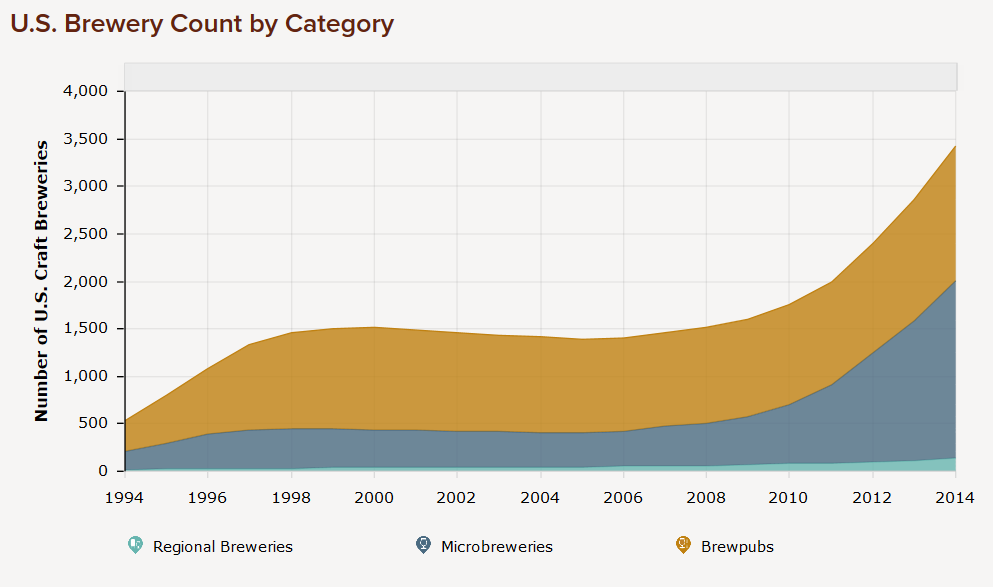
\includegraphics[scale=0.35]{./Resources/cervejarias_usa.png}
 	\captionsetup{justification=centering}
 	\caption[N�mero de cervejarias norte-americanas por categoria.]{N�mero de cervejarias norte-americanas por categoria. \\Fonte: Site da Brewers Association\protect\footnotemark
 		}
 	\label{usa-breweries}
 \end{figure}
 
 \footnotetext{Dispon�vel em \url{https://www.brewersassociation.org/statistics/number-of-breweries/}}

No Brasil, o movimento cervejeiro artesanal caseiro � considerado por algumas fontes um mercado incipiente, por�m com bom ritmo de crescimento \cite{bndes}, devido em grande parte � tend�ncia de mercado em rela��o �s microcervejarias. Desde 1995, com a funda��o da cervejaria Dado Bier, no estado do Rio Grande do Sul, que alega ser a primeira microcervejaria do Brasil \cite{revCervEd1}, seguida pela cervejaria Colorado, do estado de S�o Paulo, fundada em 1996 \cite{revCervEd2}, o movimento cervejeiro cresceu e, a partir do in�cio da d�cada de 2010 se popularizou, com estimativa de que existam atualmente cerca de 200 microcervejarias no pa�s \cite{bndes}. Esta busca por diferencia��o do consumo � refletida tamb�m no aumento do coeficiente de penetra��o de importa��es neste setor, que indica a quantidade percentual de importa��es: este cresceu de 0,02\% em 2005 para 0,21\% em 2011 \cite{bndes}. Cabe ressaltar que a ind�stria da cerveja no Brasil, como um todo, corresponde a 2\% do PIB do pa�s, representando um faturamento anual de R\$70 bilh�es \cite{cervbrasil}, portanto o mercado de artesanais, que representa cerca de 1\% do total, corresponde a um faturamento de R\$700 milh�es, com progn�stico de crescimento para 2\% em at� dez anos \cite{abrabe}.

Al�m disto, existem sistemas de produ��o autom�tica de cerveja que s�o comercializados em outros pa�ses, a exemplo do PicoBrew \cite{picobrew}, dos Estados Unidos, cuja ideia � similar � de uma cafeteira autom�tica e do Williams Warn \cite{wwarn}, da Nova Zel�ndia, que � um projeto compacto mais parecido com o equipamento de um produtor caseiro, apesar de completamente automatizado.

A motiva��o para este trabalho, portanto, surgiu a partir da constata��o de que o mercado de cervejas artesanais � crescente e rent�vel, tanto no que diz respeito a fornecer equipamentos para produtores caseiros, quanto ao fornecimento de equipamentos e tecnologia para micro e pequenas cervejarias. Outro ponto que cabe ressaltar � que a maioria das ind�strias nacionais fornecedoras de equipamentos para o mercado cervejeiro -- dentre elas Mec Bier Microcervejarias, Bierking Equipamentos, Biermatik Comercial Ltda., Cervejando.com e Mybeer, dentre outros -- oferece, na melhor das hip�teses, solu��es semi-automatizadas para opera��o presencial, a despeito das solu��es autom�ticas encontradas em outros pa�ses, o que motivou a automa��o mais complexa e remota deste trabalho. A motiva��o final deste projeto n�o � a cria��o de um produto, mas sim a compreens�o e aplica��o de tecnologias � �rea de automa��o do processo de produ��o de cerveja.

% % % % % % % % % % % % % % % % % % % % % % % % % % % % % % % % % % % % % % % % % % % % % % % % % % %
\section{Objetivos}

A descri��o do objetivo do projeto �: um sistema de Linux embarcado que automatiza o processo de produ��o de cerveja desde o cozimento do mosto at� seu resfriamento. Com rela��o ao controle e monitoramento, no sistema embarcado deve rodar um servidor web em conjunto com um algoritmo de controle autom�tico da brassagem, que forne�a ao operador do sistema uma interface web para gerenciamento de receitas e controle e monitoramento do sistema. O projeto da mec�nica do sistema tamb�m deve ser contemplado, focando em uma configura��o que permita a automa��o proposta.

Os objetivos gerais e espec�ficos do projeto foram:

\begin{itemize}
	\item Implanta��o de distribui��o Debian do Linux no sistema BeagleBone Black
	\item Interfaceamento entre o sensor DS18B20 e o sistema BeagleBone Black
	\item Projeto, aquisi��o dos componentes e montagem do sistema mec�nico
	\item Projeto do acionamento dos resistores de pot�ncia
	\item Projeto e implementa��o do programa de controle de acionamento de v�lvulas e bombas, e adi��o de ingradientes
	\item Desenvolvimento da interface web do sistema
	\item Teste e valida��o do funcionamento do sistema completo
\end{itemize}

% % % % % % % % % % % % % % % % % % % % % % % % % % % % % % % % % % % % % % % % % % % % % % % % % % %
\section {Justificativas/relev�ncia}

Este trabalho objetivou a aplica��o de conhecimentos e t�cnicas -- al�m da busca pelo estado da arte -- nas �reas de sistemas de controle, circuitos el�tricos e eletr�nicos, instrumenta��o, microcontroladores e sistemas digitais. Conhecimentos estes obtidos durante o curso de gradua��o em Engenharia El�trica - �nfase em Eletr�nica.

Outro foco foi o aprendizado de novos conhecimentos, majoritariamente nas �reas de Linux embarcado, que compreende computadores em m�dulo e SBC (\textit{single board computers} ou computadores de placa �nica), desenvolvimento de aplica��es \textit{web} e engenharia mec�nica.

Este trabalho foi importante uma vez que se prop�s a resolver problemas e criar m�todos de automa��o para uma ind�stria representativa no mercado nacional, al�m de empregar tecnologias de ponta da �rea de sistemas embarcados a uma aplica��o, fomentando o seu uso no Brasil. Do ponto de vista de cria��o de um produto, a contribui��o deixada foi o incentivo da popula��o ao \textbf{consumo consciente} de cervejas, por meio do fomento da cultura cervejeira --- bandeira levantada pelas microcervejarias artesanais nacionais, com o lema "beba menos, beba melhor", e que � de interesse da sa�de p�blica.


% % % % % % % % % % % % % % % % % % % % % % % % % % % % % % % % % % % % % % % % % % % % % % % % % % %
\section {Organiza��o do Trabalho}

Este trabalho est� distribu�do em XXX cap�tulos, incluindo esta introdu��o, dispostos conforme a descri��o que segue:

Cap�tulo 2: Descreve .....................................................................................

Cap�tulo 3: Discorre sobre .....................................................................................

Cap�tulo 4: Apresenta .....................................................................................




























%\chapter{Especifica��o do Projeto}
\label{Especificacao}

Especifica��o do projeto.


% % % % % % % % % % % % % % % % % % % % % % % % % % % % % % % % % % % % % % % % % % % % % % % % % % %
\section{Se��o 1}

Se��o dentro de um cap�tulo. 



% % % % % % % % % % % % % % % % % % % % % % % % % % % % % % % % % % % % % % % % % % % % % % % % % % %
\section{Se��o 2}

Outra se��o dentro do cap�tulo.


\chapter{Embasamento Te�rico}
\label{EmbasamentoTeorico}

Neste cap�tulo, ser� apresentado o embasamento te�rico utilizado para o desenvolvimento deste Trabalho de Conclus�o de Curso, abordando desde o processo de produ��o de cerveja e os equipamentos utilizados at� os sistemas de controle e plataforma de implementa��o da interface de usu�rio, dentre outros t�picos.

\section{Processo de Produ��o de Cerveja}

O primeiro passo para o desenvolvimento do controle de automatiza��o da produ��o de cerveja � o entendimento dos seus processos e particularidades. Esta se��o tem o objetivo de apresentar uma introdu��o � fabrica��o de cerveja, o que implica em significativas simplifica��es e resumos dos processos apresentados. Para maiores informa��es sobre o tema, recomenda-se a consulta do material bibliogr�fico de refer�ncia. 

A produ��o come�a com a escolha e \textbf{moagem} dos maltes, produzidos a partir de cereais selecionados, sendo a cevada o cereal mais amplamente utilizado -- embora outros gr�os, como trigo, centeio e aveia tamb�m possam ser empregados \cite{briggs}. O gr�o malteado � a fonte principal de a��cares ferment�veis utilizado na fabrica��o de cerveja e � produzido a partir da germina��o parcial do cereal, sendo que diferentes processos e variedades de gr�os resultam em diferentes qualidades de maltes. Estes,  por sua vez, conferem caracter�sticas �nicas aos diversos estilos de cerveja \cite{palmer,briggs}. O m�todo de moagem do malte � escolhido com base nos m�todos de brassagem e separa��o de mosto a serem empregados \cite{briggs}, e.g. em uma moagem na qual a cama de gr�os formada no processo serve como um filtro para separa��o do mosto, deve-se preservar a casca, utilizando uma moagem grossa e de macera��o, evitando tritura��o.

Com os maltes mo�dos, segue-se para a \textbf{brassagem}, que consiste na mistura de determinada quantidade de �gua quente aos maltes, possibilitando a extra��o e dilui��o dos seus a��cares ferment�veis. Enquanto um extrato em �gua fria tem rendimento na ordem de 15-22\%, o HWE (\textit{hot water extract}) -- extrato em �gua quente, chega � ordem de 75-83\% devido � atividade enzim�tica catalisadora \cite{briggs}.

O processo de brassagem pode ser realizado de v�rias maneiras, dentre elas \cite{briggs}:

\begin{enumerate}[label=(\alph*)]
	\item infus�o simples, na qual os maltes s�o cozidos a uma temperatura fixa, quase isot�rmica, utilizado tradicionalmente por cervejarias brit�nicas. � feita em uma tina de brassagem, na qual tanto o processo de extra��o dos a��cares quanto a separa��o do extrato do mosto s�o realizados. O cozimento se d� a uma temperatura na ordem de 63\textdegree C a 67\textdegree C, durante 30 minutos a duas horas e meia. O l�quido da panela (extrato) � re-circulado para que as part�culas s�lidas sejam separadas deste e, por isso, � importante que a moagem dos gr�os seja grossa, j� que estes assentam na tina e servem como filtro. Ap�s a separa��o do extrato, a cama de gr�os formada � lavada com um spray de �gua quente, processo denominado \textit{sparging};
	\item decoc��o, na qual a moagem dos gr�os � mais fina e os maltes utilizados s�o pouco modificados: devido � moagem fina, os gr�os podem ser bombeados ou misturados. Este m�todo usa tr�s recipientes: um recipiente de mistura da mostura��o, um recipiente de decoc��o e um dispositivo de separa��o do extrato do mosto. Neste processo retira-se uma quantidade de l�quido, que est� a uma temperatura inicial de 35\textdegree C, e este � fervido e adicionado novamente ao restante. Ap�s a mistura, a temperatura do mosto deve ser de cerca de 50\textdegree C e deve permanecer assim por um per�odo de tempo. O processo � repetido outras duas vezes, para obter as temperaturas de 65\textdegree C e 76\textdegree C respectivamente;
	\item dupla infus�o; e
	\item macera��o escalonada, infus�o por temperaturas programadas ou infus�o por degraus de temperatura � um processo que tem substitu�do os outros sistemas, em fun��o de sua praticidade e economia de energia, podendo economizar de 30 a 50\% com rela��o a um programa de decoc��o similar. A extra��o de a��cares � feita de forma an�loga ao processo de infus�o simples, com a diferen�a de que as temperaturas do processo s�o controladas em rampas e patamares. A filtragem do extrato do mosto pode ser feita tanto utilizando a t�cnica de cama de gr�os do processo de infus�o simples quanto a filtragem direta da decoc��o. A figura \ref{exRampa} apresenta o exemplo de tr�s programas de temperatura de brassagem - de cima para baixo, os gr�ficos da figura se referem a brassagens por degraus, decoc��o simples e decoc��o dupla. No processo por degraus, o aumento de temperatura entre os patamares deve ser da ordem de 1\textdegree C/min.
\end{enumerate}

%\newpage

\begin{figure}[H]
	\centering
	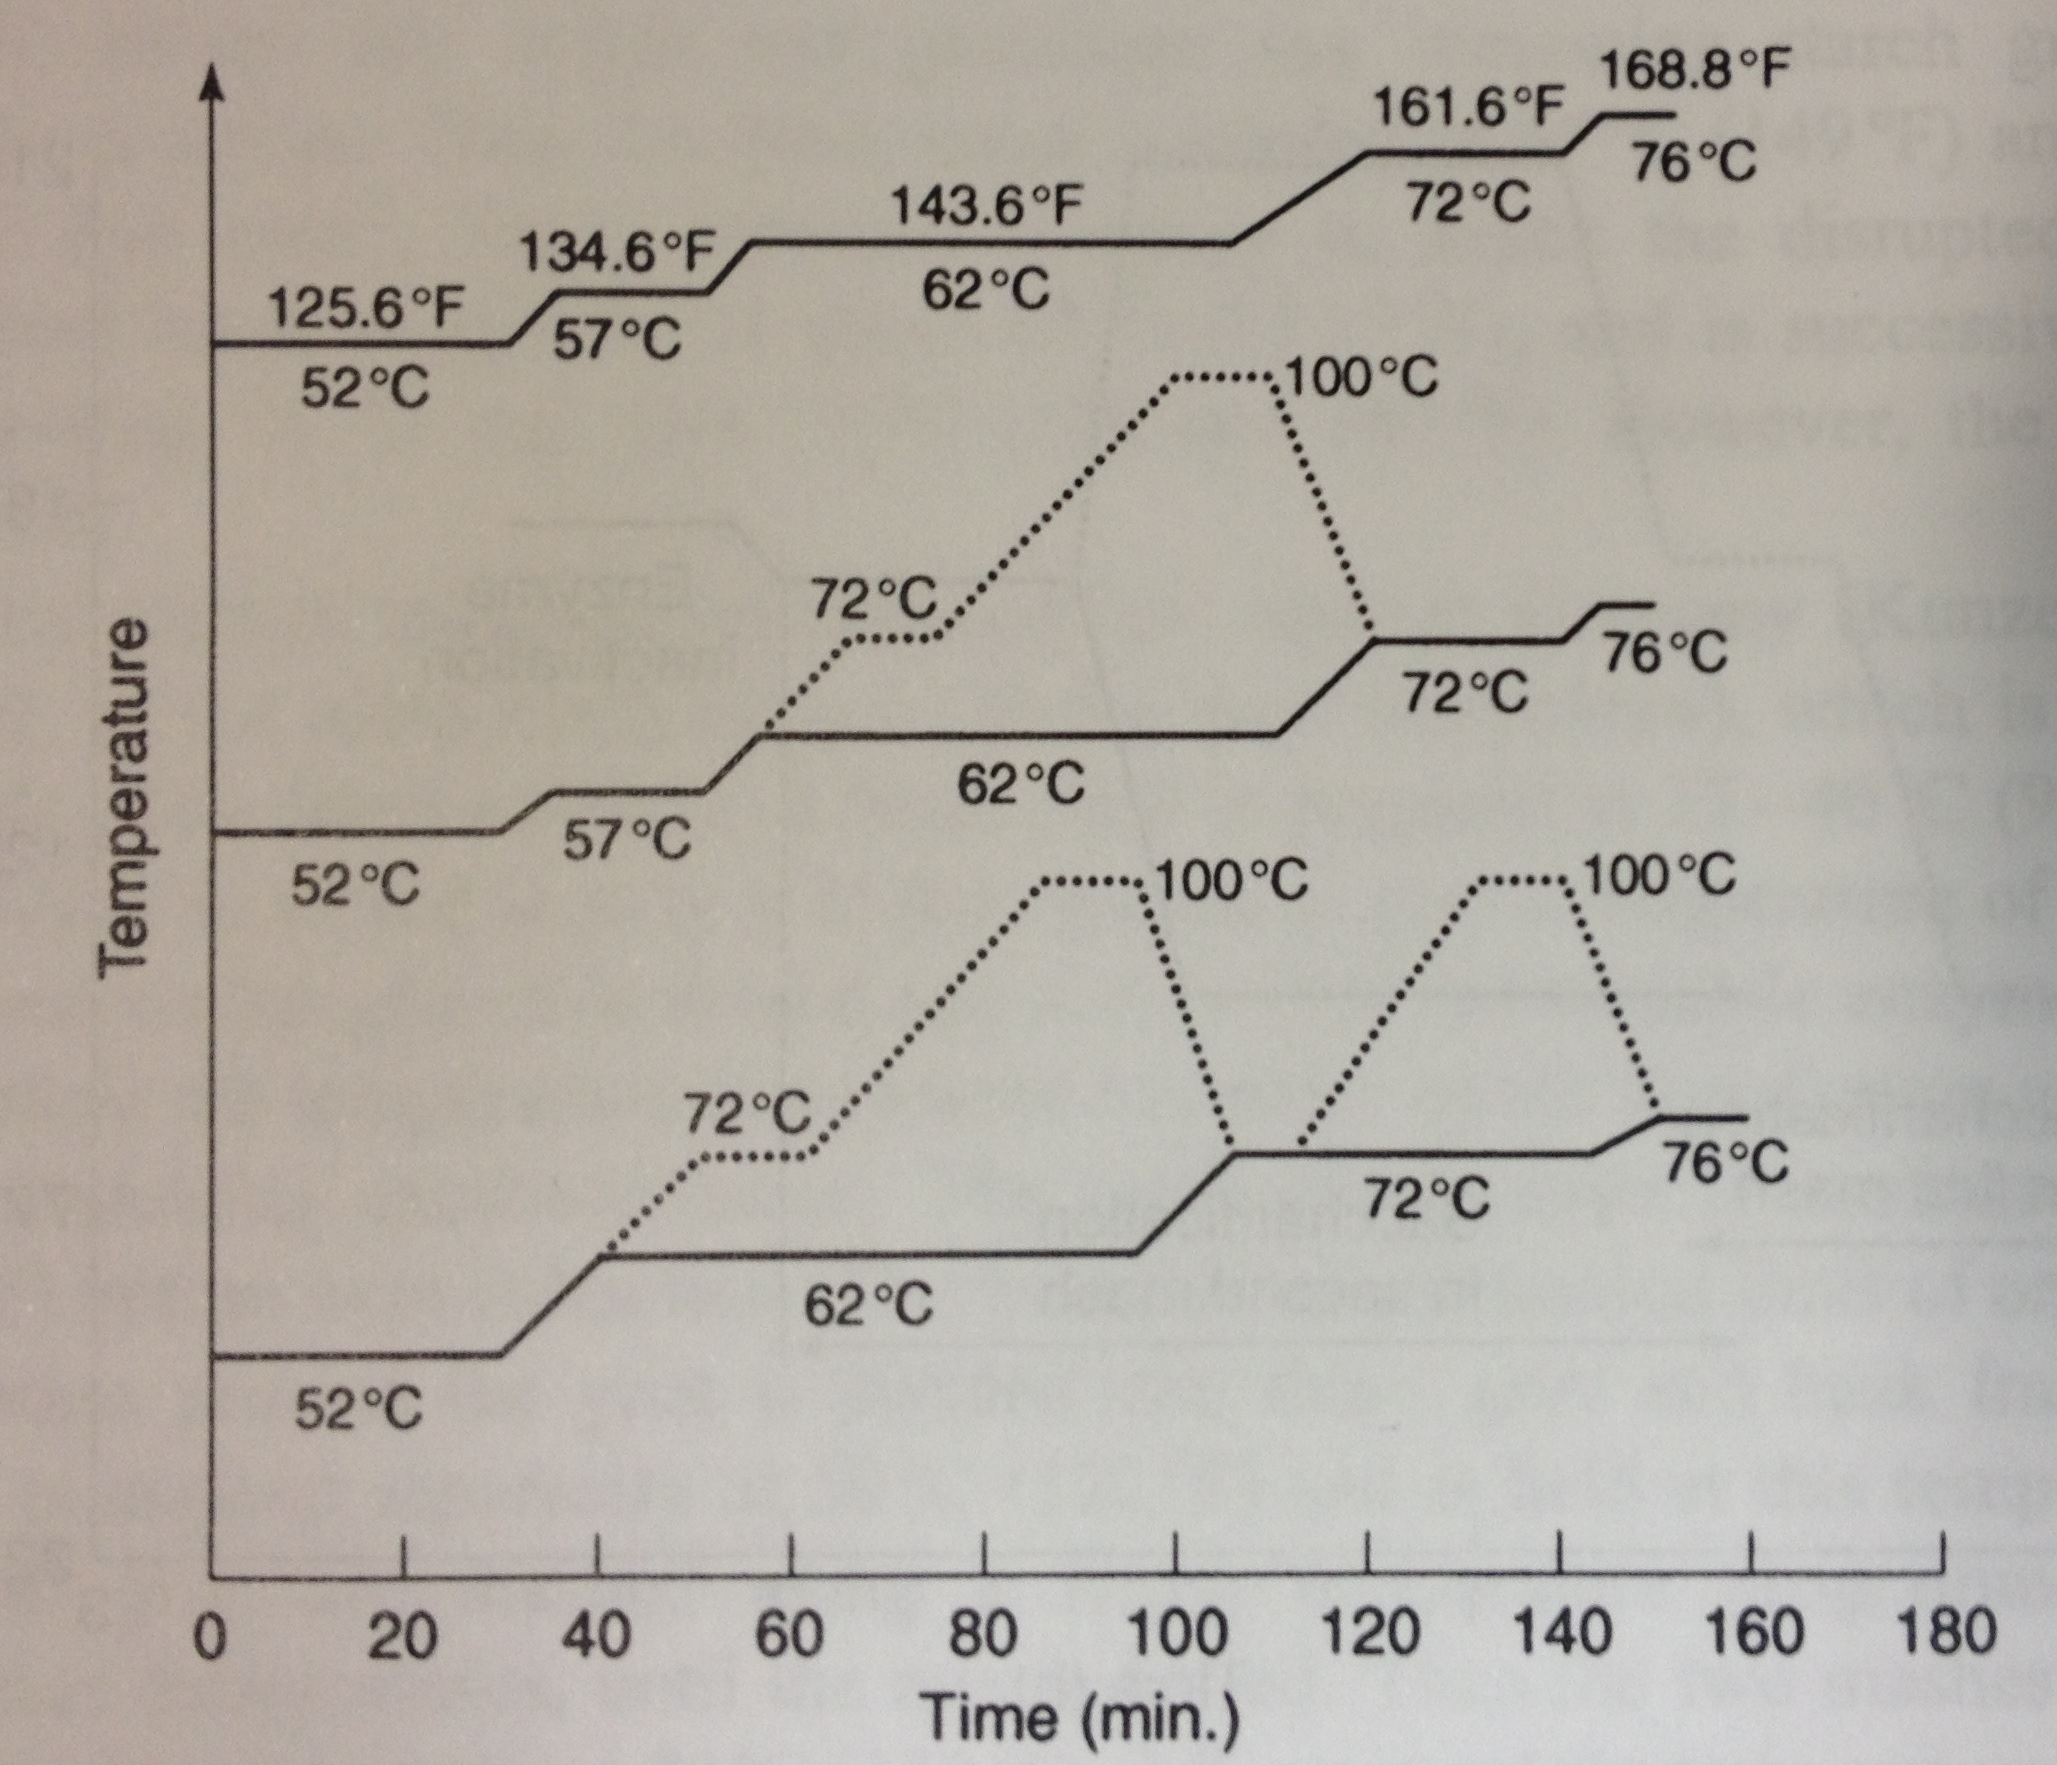
\includegraphics[scale=0.20]{./Resources/exRampas.jpg}
	\captionsetup{justification=centering}
	\caption[Programa de temperaturas t�pico de uma brassagem.]{Programa de temperaturas t�pico de uma brassagem. \\Fonte: BRIGGS (2011)
	}
	\label{exRampa}
\end{figure}

Ap�s a \textbf{filtragem} do extrato do mosto, este � transferido para um caldeir�o de \textbf{fervura}, processo no qual s�o adicionados os l�pulos e que leva cerca de uma hora, mas que pode durar mais tempo dependendo da receita \cite{briggs}, a exemplo das cervejas comerciais \textit{90 Minute IPA} e \textit{120 Minute IPA}, da cervejaria Dogfish Head, cujo tempo de fervura dura 90 minutos e 120 minutos, respectivamente \cite{1001,dogfish}. L�pulo � uma flor em formato de cone e � utilizado para conferir amargor e aroma � cerveja, al�m de ser um �timo conservante natural. Pode ser adicionado ao mosto em flores, \textit{pellets} (pastilhas prensadas) ou extrato. Quando adicionado no in�cio da fervura, contribui para o amargor da cerveja, por meio da isomeriza��o de �cidos alfa que ocorre em fun��o da alta temperatura. Em contrapartida, compostos arom�ticos vol�teis s�o perdidos neste processo e, por isso, tamb�m � adicionada uma quantidade de l�pulos ao final da fervura, para contribuir com o aroma \cite{palmer,briggs}.

Al�m de conferir amargor � cerveja, por meio da adi��o de l�pulos, a fervura tamb�m � respons�vel pela coagula��o de prote�nas indesej�veis, assepsia do l�quido, evapora��o e consequente redu��o do seu volume, mudan�as no sabor da cerveja e evapora��o de compostos vol�teis indesej�veis \cite{briggs}.

A seguir, o mosto fervido deve ser \textbf{resfriado} rapidamente at� 26\textdegree C para evitar oxida��o, contamina��o e cria��o de compostos org�nicos que introduzem sabores indesejados \cite{palmer}. O processo de resfriamento � realizado com o emprego de um trocador de calor, denominado \textit{chiller}. Tamb�m devem ser separadas e desprezadas as prote�nas coaguladas e os restos de l�pulos decorrentes da fervura. Este processo geralmente � denominado \textit{whirlpool}, em fun��o de sua natureza, na qual o mosto fervido � centrifugado e os compostos indesejados se acumulam no centro e no fundo da panela de fervura \cite{briggs}. O �ltimo passo � aerar ou at� mesmo oxigenar o mosto, para que as leveduras possam se reproduzir corretamente no in�cio da \textbf{fermenta��o} \cite{briggs}.

A levedura deve ser adicionada ao mosto resfriado e oxigenado o mais r�pido poss�vel para evitar contamina��es, e o recipiente de fermenta��o comumente � selado, evitando a entrada de ar \cite{briggs}. O processo de fermenta��o e os subsequentes processos de \textbf{matura��o} e \textbf{envase} n�o ser�o detalhados, pois sua automa��o n�o � parte do escopo deste trabalho. 

\section{Estrutura mec�nica}

O processo de brassagem, que consiste no cozimento dos maltes para extra��o dos a��cares ferment�veis e filtra��o do l�quido resultante, conhecido como mosto, � realizado em equipamentos espec�ficos para estas tarefas. Em fun��o das diferentes t�cnicas de brassagem e tecnologias desenvolvidas ao longo do tempo, diversos tipos e arranjos de equipamentos foram desenvolvidos \cite{briggs}.

Atualmente existe uma converg�ncia nos m�todos de fabrica��o de cervejas, motivada principalmente por quest�es financeiras, cujo objetivo do equipamento � maximizar a produ��o. Outros motivos para o desenvolvimento e aprimoramento de equipamentos s�o a necessidade de sempre produzir uma cerveja com as mesmas caracter�sticas, ou seja, padronizar a produ��o e, tamb�m, a preocupa��o crescente com redu��o do uso de energia e �gua e a redu��o da produ��o de efluentes \cite{briggs}. Ainda assim, equipamentos antigos continuam em uso, seja pela impossibilidade de reproduzir a cerveja em equipamentos mais modernos ou pelo custo elevado da atualiza��o das plantas de produ��o.

Na adi��o dos gr�os � panela de mostura, o processo de mistura destes � �gua � importante para que a brassagem seja eficiente, uma vez que os gr�os mal misturados podem formar aglutinados que impedem a extra��o dos a��cares. Para evitar este inconveniente, dispositivos mec�nicos foram desenvolvidos, conforme exposto na figura \ref{mashin}: em (a) a �gua e os gr�os s�o misturados em um fluxo constante, determinado pela velocidade de giro de uma rosca sem fim e; em (b) a �gua � adicionada aos maltes em um �ngulo tangente, de tal forma que um v�rtex a mistura aos gr�os.  A temperatura da �gua tamb�m deve ser controlada, para evitar que prote�nas sejam inativadas e seu volume inicial � predeterminado conforme a receita \cite{briggs}.

\begin{figure}[H]
	\centering
	\begin{subfigure}{.59\textwidth}
		\centering
		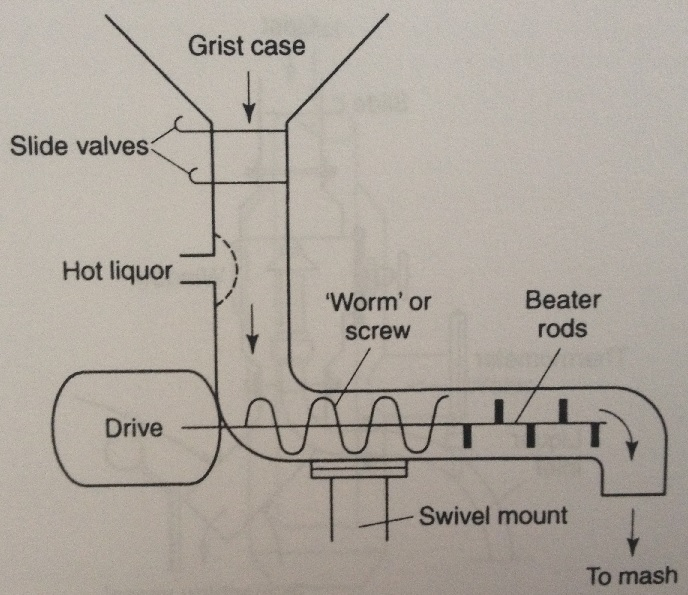
\includegraphics[height=5cm]{./Resources/mashin.jpg}
		\caption{Dispositivo com rosca sem fim}
		\label{mashin:1}
	\end{subfigure}
	\begin{subfigure}{.4\textwidth}
		\centering
		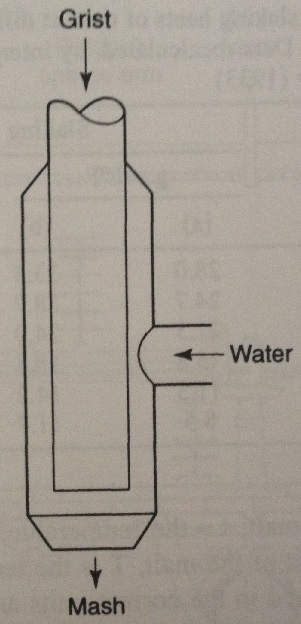
\includegraphics[height=5cm]{./Resources/mashin1.jpg}
		\caption{Dispositivo de mistura por v�rtex}
		\label{mashin:2}
	\end{subfigure}
	\captionsetup{justification=centering}
	\caption[Dispositivos de mistura de gr�os � brassagem.]{Dispositivos de mistura de gr�os � brassagem. \\Fonte: BRIGGS (2011)
	}
	\label{mashin}
\end{figure}

\subsection{Panela de mostura}

A panela de mostura, ou MT (\textit{mash tun}), � o dispositivo mais simples para a prepara��o do mosto, uma vez que nela ocorre a extra��o dos a��cares, a filtra��o do extrato do mosto e a lavagem dos gr�os \cite{briggs}. A figura \ref{mashTun} apresenta uma configura��o comum de MT, usada atualmente.

\begin{figure}[H]
	\centering
	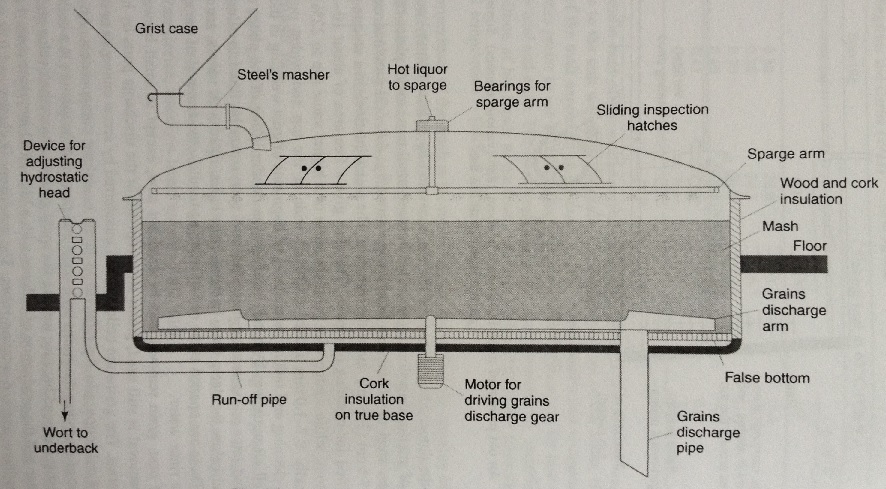
\includegraphics[scale=0.55]{./Resources/mt_modern.jpg}
	\captionsetup{justification=centering}
	\caption[Esquema de panela de brassagem industrial moderna.]{Esquema de panela de brassagem industrial moderna. \\Fonte: BRIGGS (2011)
	}
	\label{mashTun}
\end{figure}

As MTs possuem se��o transversal circular e atualmente s�o feitas de a�o inoxid�vel, revestidas com material isolante t�rmico. Embora originalmente fossem abertas, atualmente s�o cobertas para evitar perda de calor e espalhamento do vapor de �gua pelo ambiente da brassagem. O fundo da MT � coberto por um fundo falso, que fica a alguns cent�metros acima do fundo original e cuja fun��o � atuar como filtro, em conjunto com a cama de gr�os. Este fundo falso consiste de uma ou mais chapas de metal com rasgos da ordem de 0,7-1,0mm, que representam uma �rea livre para a drenagem de cerca de 12\% da �rea total, ou uma trama com fios de metal cuja �rea livre chega a 22\% \cite{briggs}.

O descarte dos gr�os � feito atrav�s de um tubo, com a ajuda de uma p� que varre o fundo da panela ou um jato de ar comprimido. M�todos de remo��o dos gr�os descontinuados s�o a remo��o manual (que ainda existe em pequenas instala��es) e o enx�gue dos gr�os com bombeamento para um tanque anexo -- este n�o mais usado em fun��o da necessidade de mais �gua e posterior tratamento desta, que resulta em custos adicionais, al�m da perda do valor comercial dos gr�os a serem descartados. Com rela��o � limpeza, as MTs s�o constru�das com suporte � limpeza CIP (limpeza no local), inclusive na regi�o entre o fundo da panela e o fundo falso \cite{briggs}.

A �gua da lavagem dos gr�os, ou \textit{sparging}, � borrifada por um cano ou mais canos suspensos acima da cama de gr�os, conforme ilustrado na figura \ref{mashTun}. Estes canos s�o conhecidos como bra�os de \textit{sparging} e geralmente giram no eixo em fun��o da for�a da �gua, o que s� � poss�vel devido aos furos no tubo serem feitos na vertical, especialmente para este prop�sito. Outro aspecto da constru��o dos bra�os de \textit{sparging} � que, � medida que se aproxima do centro da panela, os furos s�o feitos a uma dist�ncia menor entre si, possibilitando que a �gua seja igualmente distribu�da sobre a cama de gr�os \cite{briggs}. O extrato do mosto � coletado por tubos no fundo da panela.

No caso da brassagem feita pelo processo de decoc��o, brassagem dupla ou infus�o por temperatura controlada, diferentes recipientes de brassagem s�o utilizados. A figura \ref{mashMixer} � um exemplo de tina de mistura (n�o confundir com mostura, embora a panela seja utilizada no processo de mostura) usada para brassagem de temperatura controlada. Nestes casos, a moagem dos maltes � mais fina e estes s�o constantemente misturados por uma p� no fundo da panela. Mesmo dentre estes sistemas os equipamentos diferem entre si e, diferente da MT, nestes sistemas � preciso utilizar outro recipiente para separar o extrato dos gr�os. O separador pode ser uma tina de lavagem, conhecida tamb�m como LT (\textit{lauter tun}), ou pode ser um filtro de mosto. Embora a LT e o filtro de mosto sejam amplamente utilizados na ind�stria, n�o ser�o detalhados neste trabalho, j� que a abordagem pr�tica adotada n�o inclui seu uso.

\begin{figure}[H]
	\centering
	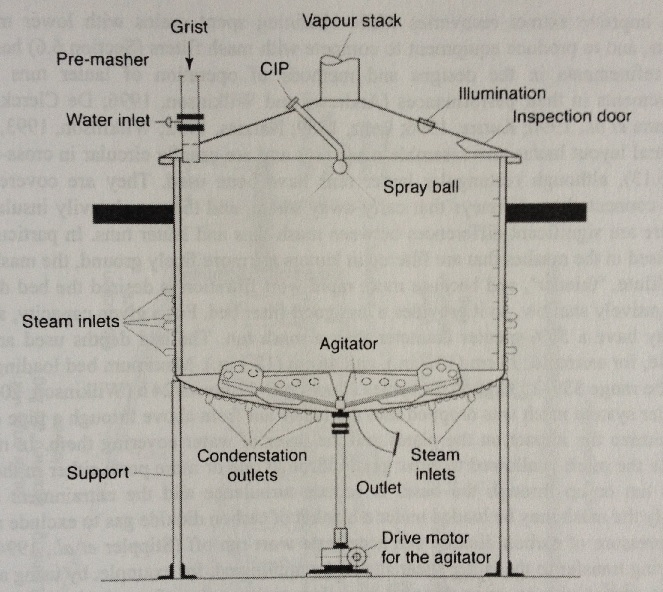
\includegraphics[scale=0.55]{./Resources/mt_mix.jpg}
	\captionsetup{justification=centering}
	\caption[Esquema de panela de mistura do mosto.]{Esquema de panela de mistura do mosto. \\Fonte: BRIGGS (2011)
	}
	\label{mashMixer}
\end{figure}

\subsection{Caldeir�o de fervura}

A fervura � o processo no qual o extrato do mosto � fervido com a adi��o de l�pulos em um caldeir�o de fervura. Em ingl�s o termo utilizado para este caldeir�o (\textit{copper}, que significa cobre) lembra o fato de que inicialmente era comum o emprego de tinas de cobre, dada a facilidade de moldagem que este metal permite, a alta condutividade t�rmica e a apar�ncia atrativa dos caldeir�es \cite{briggs}. Este tamb�m � usualmente referido como BK, ou \textit{brewing kettle} (caldeir�o de fervura). Por muito tempo o estudo do processo de fervura foi negligenciado por ser considerado simples, mas � medida que a quest�o da economia de energia veio � pauta, estudos oriundos desta necessidade mostraram que o processo � mais complicado do que foi inicialmente considerado \cite{briggs}.

Como existe uma lista de objetivos que devem ser cumpridos durante o processo de fervura, o projeto do equipamento � essencial para que estes sejam atingidos e, em um grau mais avan�ado, a maior economia de energia possa ser obtida. O primeiro objetivo -- que n�o est� necessariamente em ordem de import�ncia -- � a evapora��o de �gua e consequente concentra��o do mosto, com taxas de evapora��o inicialmente na faixa de 10\% do volume por hora e que foram reduzidas com o desenvolvimento tecnol�gico das grandes ind�strias, j� que o custo de evapora��o da �gua � caro em termos de demanda energ�tica. O segundo objetivo importante da fervura � esterilizar o mosto, ou pelo menos matar formas vegetativas de micr�bios -- ainda que esporos possam sobreviver ao processo. A terceira fun��o do processo � a evapora��o de compostos vol�teis indesejados, o que resultou em um desafio tecnol�gico para diminuir os tempos de fervura e quantidade de �gua evaporada sem que os compostos vol�teis deixassem de ser eliminados efetivamente \cite{briggs}.

Dentre as mudan�as que ocorrem no mosto durante a fervura, podem ser notadas cria��es, adi��es e transforma��es de subst�ncias qu�micas, como a dispers�o de resinas e �leos do l�pulo no mosto e a isomeriza��o de �cidos-\si{\alpha} (transforma��o dos �cidos-\si{\alpha} presentes no l�pulo em is�meros que conferem caracter�sticas de amargor � bebida), al�m da desnatura��o e forma��o de co�gulos de prote�nas -- processo que � favorecido por uma fervura rigorosa e prolongada -- que vir�o a formar o chamado \textit{trub}, resultado da decanta��o destas prote�nas.  Este processo de decanta��o pode ser acelerado por meio da adi��o de subst�ncias como gel de s�lica ou musgo irland�s, conhecido como \textit{irish moss} \cite{briggs}.

Historicamente o aquecimento dos BKs era feito de forma direta, com a queima de combust�veis s�lidos. Embora estes n�o sejam empregados atualmente, ainda existem BKs que s�o aquecidos diretamente, por meio da queima de �leos ou gases. Ainda assim, atualmente o maior elemento de aquecimento utilizado � o vapor d'�gua. Embora estes sistemas sejam mecanicamente mais complexos, o aquecimento a vapor reduz a quantidade de calor aplicada por unidade de �rea, o que evita a carameliza��o do mosto \cite{briggs}. Na figura \ref{boilcopper} s�o apresentadas tr�s configura��es de BKs, sendo (a) e (b) por meio de aplica��o direta de vapor � superf�cie do recipiente e (c) utilizando um aquecedor interno, tamb�m a vapor.

\begin{figure}[H]
	\centering
	\begin{subfigure}{.46\textwidth}
		\centering
		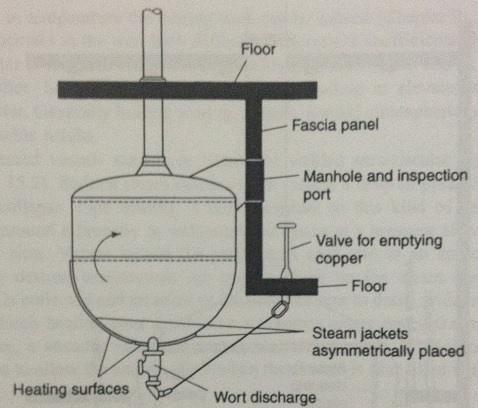
\includegraphics[height=5cm]{./Resources/boil_steam1.jpg}
		\caption{Caldeir�o com base arredondada e revestimentos de vapor assimetricamente dispostos}
		\label{boilcopper:1}
	\end{subfigure}
	\begin{subfigure}{.46\textwidth}
		\centering
		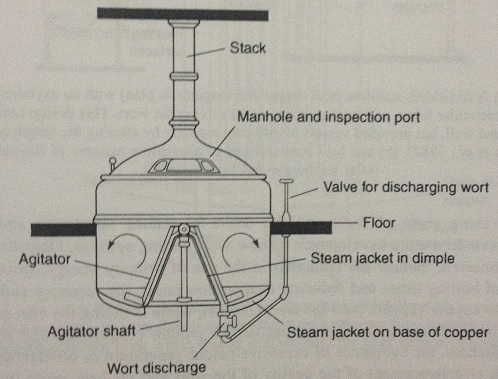
\includegraphics[height=5cm]{./Resources/boil_steam2.jpg}
		\caption{Caldeir�o de alta efici�ncia, com revestimentos de vapor na base e no cone central}
		\label{boilcopper:2}
	\end{subfigure}
	\begin{subfigure}{.65\textwidth}
		\centering
		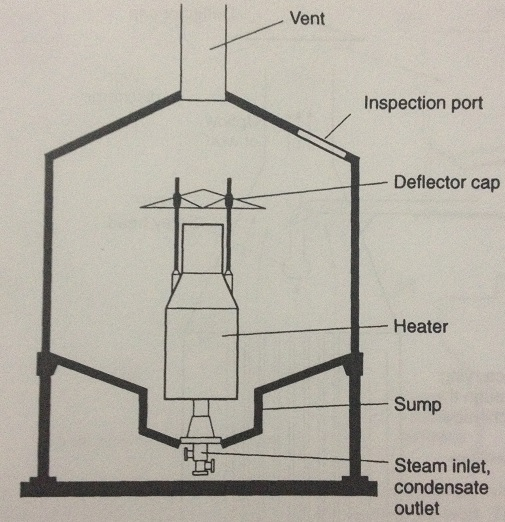
\includegraphics[height=5cm]{./Resources/boil_internal.jpg}
		\caption{Caldeir�o com aquecimento interno e mais profundo no centro, permitindo um aquecedor maior}
		\label{boilcopper:3}
	\end{subfigure}
	\captionsetup{justification=centering}
	\caption[Diferentes configura��es de caldeir�es de fervura.]{Diferentes configura��es de caldeir�es de fervura. \\Fonte: BRIGGS (2011)
	}
	\label{boilcopper}
\end{figure}

O projeto destes sistemas mec�nicos s�o feitos com o objetivo de evitar que o mosto seja caramelizado ou descaracterizado de alguma forma e de modo a economizar energia. Com isso surgiram em fun��o do tempo sistemas pressurizados e de aquecimento externo do l�quido, dentre outras configura��es diversas. Todos os sistemas modernos e eficientes de fervura s�o fechados e se aproveitam da pressuriza��o de algum modo para reduzir o custo energ�tico do processo de fervura, que se d� pela redu��o do tempo de fervura possibilitada pela eleva��o da temperatura do mosto. Contudo � preciso atentar-se ao fato de que temperaturas muito altas podem afetar negativamente a produ��o da cerveja e, portanto, valores t�picos de temperatura empregados pela ind�stria chegam a at� 104\si{\degree}C, com exce��es\footnotemark \cite{briggs}. A tabela \ref{tipos_fervura} apresenta alguns sistemas de fervura utilizados na ind�stria e suas caracter�sticas com rela��o a temperatura, tempo de fervura e evapora��o do mosto. Note-se que mesmo para um tipo espec�fico de fervura, diversas configura��es de equipamento podem ser adotadas.

\footnotetext{O sistema de alta temperatura / alta press�o (140\si{\degree}C) � pouco utilizado e testes pr�ticos mostram que os resultados em termos de qualidade da cerveja s�o question�veis \cite{briggs}}

\begin{center}
	\begin{table}[H]
		\captionsetup{justification=centering}
		\caption[Caracter�sticas de diferentes sistemas de fervura.]{Caracter�sticas de diferentes sistemas de fervura. \\Fonte: adaptado de BRIGGS(2011)}
		\label{tipos_fervura}
		\begin{tabular}{ | M{6cm}  M{3cm}  M{3cm}  M{3cm} |}
			\hline
			\textbf{Sistema de aquecimento} & \textbf{Temperatura (\si{\degree}C)} & \textbf{Tempo de fervura (min.)} & \textbf{Evapora��o (\%)} \\ \hline
			Panela de "alta performance" & 100 & 120-150 & 12-16 \\
			Aquecedores internos/externos, com contrapress�o & 102-103 & 60-80 & 8 \\
			Fervura de baixa press�o & 103-104 & 55-65 & 6-7 \\
			Fervura din�mica de baixa press�o & 103-104 & 45-50 & 4,5-5 \\
			Fervura de alta temperatura / alta press�o & 130-140 & 2,5-3 & 6-8 \\
			Aquecimento de pel�cula fina & 100 & 35-40 & 4-4,7\\ \hline
		\end{tabular}
	\end{table}
\end{center}

Embora o objetivo principal deste trabalho n�o seja a efici�ncia energ�tica do sistema, neste par�grafo s�o apresentadas algumas considera��es acerca do tema. Uma vez que o aquecimento de �gua une todas as partes do processo de produ��o de cerveja, n�o � realista acreditar que a economia de energia pode ser aplicada exclusivamente ao processo de fervura, que � o mais custoso em termos energ�ticos, portanto automa��o de controles, equipe bem capacitada, boa conserva��o do edif�cio, \textit{designs} eficientes, dentre outros fatores, s�o importantes para a economia de energia. No tocante � fervura em espec�fico, geralmente s�o utilizados sistemas que recuperam energia de vapor e/ou �gua quente para reuso nas diversas etapas do processo de produ��o de cerveja \cite{briggs}. Um exemplo � o sistema da figura \ref{eng_sav}, que utiliza energia do vapor de aquecimento utilizado na fervura para posterior aquecimento do mosto e pr�-aquecimento de outra fervura. Para que isto seja poss�vel, � essencial que a cervejaria realize consecutivas produ��es, uma vez que a energia � transferida para a produ��o seguinte.

\newpage

\begin{figure}[H]
	\centering
	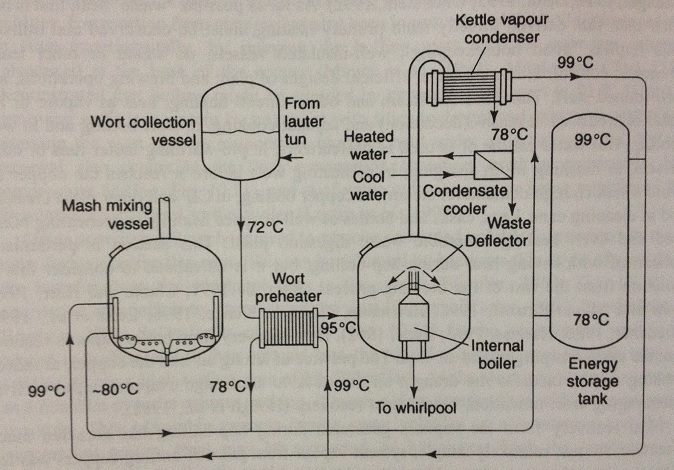
\includegraphics[scale=0.5]{./Resources/energy_saving.jpg}
	\captionsetup{justification=centering}
	\caption[Arranjo para recupera��o de energia.]{Arranjo no qual vapor do caldeir�o de fervura � condensado e calor � recuperado e armazenado como �gua quente em um tanque de gradiente de temperatura. \\Fonte: BRIGGS (2011)
	}
	\label{eng_sav}
\end{figure}

\subsection{Adi��o de l�pulos}

� comum realizar a adi��o de l�pulos manualmente em pequenas cervejarias, por�m deve-se observar que a adi��o de l�pulos pode ser uma tarefa perigosa, pois o mosto pode subitamente vazar. Tamb�m, em adi��es tardias de l�pulo, ocorre a entrada de ar no BK, o que faz com que sistemas pressurizados n�o possam ser utilizados sem as devidas considera��es e/ou modifica��es no equipamento \cite{briggs}.

A adi��o de l�pulos geralmente n�o � satisfat�ria quando s�o utilizadas flores, por isso pastilhas ou extratos s�o geralmente utilizados. Em grandes cervejarias a maior parte do desafio est� no fato de que os l�pulos devem ser armazenados em ambientes com temperatura controlada, que geralmente ficam longe do BK, al�m de serem armazenados em caixas ou tanques. Al�m do sistema autom�tico de transporte destes pacotes, em caso de BKs com pressuriza��o, � preciso utilizar sistemas de c�maras de compress�o para adicionar os l�pulos � panela \cite{briggs}.

\subsection{Clarifica��o e resfriamento do mosto}
Quando o processo de fervura � finalizado, o mosto dever� estar claro, ou seja, com apar�ncia brilhante. Ainda assim, � preciso remover o \textit{trub}\footnotemark \footnotetext{O \textit{trub} descrito neste cap�tulo � referente ao \textit{hot break}, ou processo de fervura. Neste trabalho n�o ser� abordado o \textit{trub} decorrente do \textit{cold break}, ou resfriamento do mosto, que come�a a ser formado em temperaturas pr�ximas a 70\si{\degree}C} e os restos de l�pulos utilizados no processo, j� que o \textit{trub} contribui com compostos sulfurosos e alco�is indesejados, al�m de tornar a cerveja turva -- o que pode ou n�o ser um problema \cite{byown}. Diversos equipamentos foram criados com este prop�sito, seja para mostos com adi��o de l�pulos em flores, que facilitam a extra��o dos compostos indesej�veis, quanto para mostos feitos com pastilhas e extratos de l�pulo. H� sistemas chamados \textit{hop back} empregados na filtragem de mostos com l�pulos em flor e que lembram MTs, nos quais o mosto � filtrado por um fundo falso, com elemento filtrador sendo a cama de l�pulos que decanta para o fundo da panela -- inclusive h� pequenas cervejarias que utilizam a MT para realizar este m�todo de clarifica��o \cite{briggs}.

Embora existam outros sistemas de clarifica��o, o empregado mais largamente na ind�stria atual � a t�cnica de \textit{whirlpool} (redemoinho, em tradu��o livre) na qual mosto quente � injetado tangencialmente em um recipiente cil�ndrico, a uma velocidade fixa, sendo a altura de inje��o do mosto vari�vel em fun��o de diferentes projetos. Sistemas de gravidade geralmente n�o s�o suficientes e bombas ou sistemas projetados para utilizar o efeito de termossif�o s�o utilizadas. As correntes de circula��o do mosto decorrentes desta inje��o tangencial fazem com que o material particulado fique concentrado no fundo e no centro do recipiente, possibilitando o escoamento controlado do l�quido e a consequente separa��o do \textit{trub} \cite{briggs}. Na figura \ref{whirlpool} s�o ilustrados sistemas de separa��o por decanta��o (a) e por \textit{whirlpool} (b).


\begin{figure}[H]
	\centering
	\begin{subfigure}{1.0\textwidth}
		\centering
		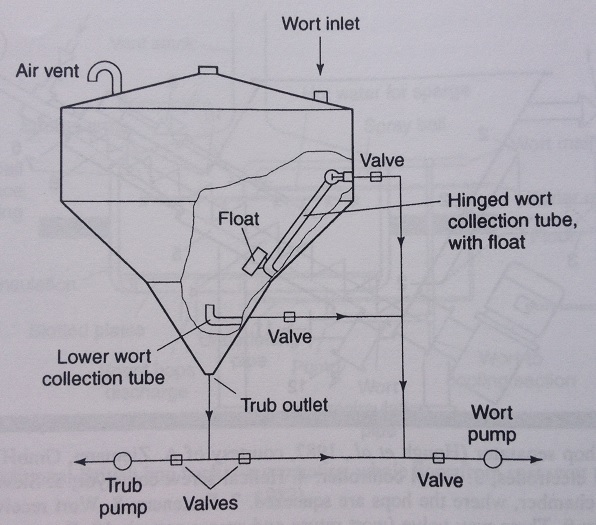
\includegraphics[height=5cm]{./Resources/trub_decanter.jpg}
		\caption{Sistema de serapa��o do \textit{trub} por decanta��o}
		\label{whirlpool:1}
	\end{subfigure}
	\begin{subfigure}{1.0\textwidth}
		\centering
		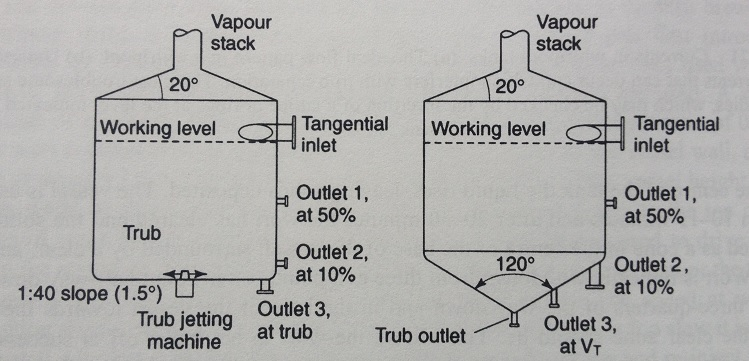
\includegraphics[height=5cm]{./Resources/trub_whirlpool.jpg}
		\caption{Sistemas de separa��o do \textit{trub} por \textit{whirlpool}, com fundo plano e arredondado}
		\label{whirlpool:2}
	\end{subfigure}
	\captionsetup{justification=centering}
	\caption[Sistemas de clarifica��o.]{Sistemas de clarifica��o. \\Fonte: BRIGGS (2011)
	}
	\label{whirlpool}
\end{figure}

Ap�s o processo de clarifica��o deve come�ar a fermenta��o e, para que as leveduras possam ser inoculadas no mosto, este deve ser resfriado at� a temperatura ideal de opera��o destes microorganismos, que est� t�picamente na faixa 15-22\si{\degree}C para leveduras do tipo \textit{ale} e 6-12\si{\degree}C para leveduras do tipo \textit{lager}. O resfriamento r�pido do mosto deve ocorrer, pois assim rea��es qu�micas decorretes da fervura s�o interrompidas e a chance de contamina��o do mosto � reduzida \cite{briggs}.

Para isto, um \textit{cooler} (resfriador ou trocador de calor) � utilizado. Dentre os modelos mais largamente empregados encontra-se o \textit{cooler} vertical, no qual o mosto passa por dentro de um arranjo de tubos finos, enquanto na parte externa destes �gua fria � circulada em contra-fluxo. Ainda assim, o modelo de \textit{cooler} mais popular � do trocador de calor de placas, devido ao seu tamanho compacto, versatilidade e efici�ncia. As placas possuem padr�es de desenho de tal forma que, quando s�o compactadas, elas formam canais pelos quais o mosto � passado em contra-fluxo a um agente resfriador (�gua fria, por exemplo). Estes trocadores de calor s�o projetados para que o escoamento seja turbulento e, consequentemente, a troca de calor seja mais eficiente. Quando um agente resfriador diferente da �gua � utilizado, a manuten��o do sistema deve ser refor�ada, j� que vazamentos implicam na contamina��o do mosto \cite{briggs}. A figura apresenta um esquema de \textit{cooler} de placas.

 \begin{figure}[H]
 	\centering
 	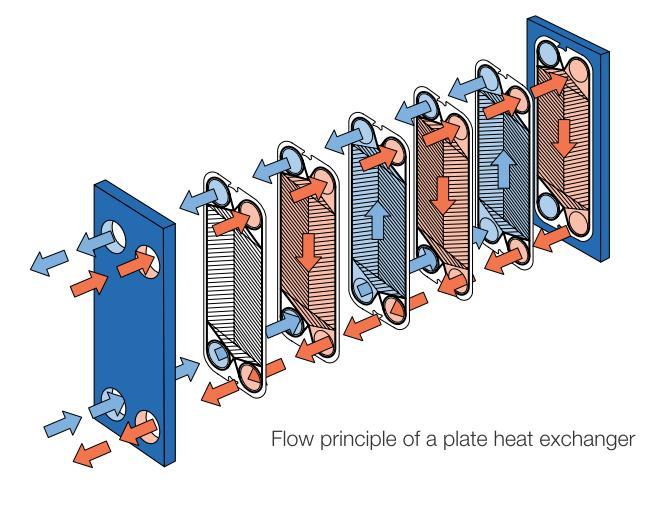
\includegraphics[scale=0.55]{./Resources/cooler.jpg}
 	\captionsetup{justification=centering}
 	\caption[Esquema de funcionamento do trocador de calor de placas.]{Esquema de funcionamento do trocador de calor de placas. \\Fonte: Site da Offshore Energy Today\protect\footnotemark
 	}
 	\label{usa-breweries}
 \end{figure}
 
 \footnotetext{Dispon�vel em \url{http://www.offshoreenergytoday.com/wp-content/uploads/2012/03/Alfa-Laval-to-Supply-Plate-Heat-Exchangers-for-Brazilian-Offshore-Plaforms.jpg}}

Por fim, antes de inocular a levedura, � importante que o mosto seja suficientemente aerado ou oxigenado. Sem isso, a levedura n�o ter� um ambiente adequado � sua reprodu��o e a atenua��o do mosto -- transforma��o de a��cares e oxig�nio em �lcool e g�s carb�nico -- n�o ser� completada. Diferen�as de solubilidade do mosto e dos tipos de levedura podem influenciar na quantidade de oxig�nio necess�ria para um bom andamento da fermenta��o, sendo que para obter os n�veis adequados, em escala industrial a oxigena��o geralmente � for�ada  \cite{briggs,palmer}. Na produ��o de cerveja artesanal, a aera��o geralmente � feita agitando o mosto resfriado ou com a ajuda de um sistema de aera��o de aqu�rio \cite{palmer}.

\section{BeagleBone Black}

BBB � uma placa de sistema embarcado desenvolvida para a comunidade de c�digo aberto (\textit{open-source}), iniciantes e quaisquer pessoas interessadas em um sistema equipado com um processador ARM Cortex-A8 32-bits de baixo custo, seja para teste de conceito ou mesmo uso pessoal/profissional. Embora o sistema tenha sido desenvolvido com um n�mero reduzido de funcionalidades, de modo a proporcionar uma boa experi�ncia de uso, esta placa n�o � uma plataforma completa de desenvolvimento nem � voltada para o desenvolvimento de um produto espec�fico, mas sim para a experimenta��o e aprendizado nas �reas de \textit{software} e \textit{hardware} \cite{bbb_srm}. A figura \ref{bbb} apresenta a placa e seus principais componentes, em conjunto com a tabela \ref{bbb_specs}, onde est�o contidas as especifica��es gerais de hardware e a figura \ref{bbb-bdg}, na qual est� contido um diagrama de blocos do sistema, de alto n�vel de abstra��o. O diagrama esquem�tico do sistema pode ser obtido no Anexo \ref{Anexo1}.

� imprescind�vel atentar para o fato de que a BBB possui diversas revis�es de \textit{hardware}, sendo que a vers�o utilizada neste trabalho � a \textbf{revis�o C}.

A combina��o do processador ARM Cortex-A8 com o projeto de \textit{hardware} da placa possibilita o uso de um sistema operacional embarcado -- geralmente uma distribui��o Linux -- que fornece facilidades de programa��o, a exemplo de uma IDE acessada pelo navegador da internet chamada Cloud9 em combina��o com uma biblioteca de acesso ao hardware em \textit{server-side} Javascript (Node.js), possibilitando a prototipagem r�pida de solu��es embarcadas de produtos voltados ao mundo real. � medida que o desenvolvedor do sistema se torna mais experiente, � poss�vel desenvolver solu��es mais complicadas em diversas linguagens de programa��o, utilizando-se para isto do sistema operacional Linux embarcado na placa. \cite{bbb_nannan}. Al�m disso, projetos como o do carro de controle remoto via web, desenvolvido por \cite{bbb_nannan} com o intuito de confirmar as capacidades de placa e seu potencial uso no ensino de sistemas embarcados, refor�am a escolha da BBB como plataforma para este projeto.  

\begin{figure}[H]
	\centering
	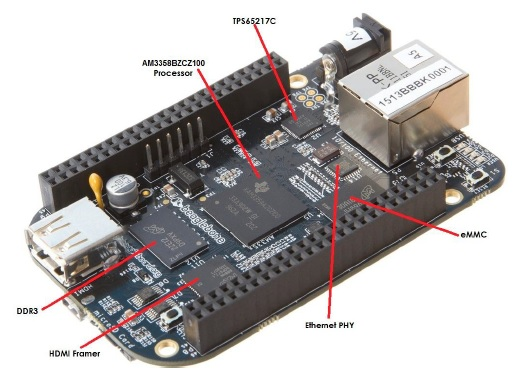
\includegraphics[scale=0.55]{./Resources/bbb-components.jpg}
	\captionsetup{justification=centering}
	\caption[BeagleBone Black e principais componentes]{BeagleBone Black e principais componentes. \\Fonte: COLEY (2014)
	}
	\label{bbb}
\end{figure}

\begin{itemize}
	\item \textbf{Sitara AM3358BZCZ100} - SoC (\textit{system on chip})
	\item \textbf{Micron 512MB DDR3L ou Kingston 512MB DDR3} - mem�ria RAM
	\item \textbf{TPS65217C PMIC} - controlador de alimenta��o dos diferentes componentes do sistema
	\item \textbf{SMSC Ethernet PHY} - interface f�sica � rede Ethernet
	\item \textbf{Micron eMMC} - mem�ria n�o vol�til MMC de 4GB
	\item \textbf{HDMI Framer} - controlador para uso com display HDMI ou DVI-D
\end{itemize}

\begin{center}
	\begin{table}[H]
		\captionsetup{justification=centering}
		\caption[Especifica��es Gerais da BeagleBone Black]{Especifica��es Gerais da BeagleBone Black. \\Fonte: adaptado de COLEY(2014)}
		\label{bbb_specs}
		\begin{tabular}{ | M{3cm} | M{12cm} |}
			\hline
			& \multicolumn{1}{|c|}{\textbf{Especifica��o}} \\ \hline
			Processador & Sitara AM3358BZCZ100, 1GHz, 2000 MIPS\\ \hline
			Motor Gr�fico & SGX530 3D, 20M pol�gonos/s \\ \hline
			Mem�ria SDRAM & 512MB DDR3L 800MHz \\ \hline
			Mem�ria Flash & 4GB, 8bit MMC embarcada \\ \hline
			CI Gerenciador de Alimenta��o & TPS65217C + regulador adicional (linear) \\ \hline
			Suporte a \textit{debug} & Interface serial, Conector CTI JTAG opcional de 20 pinos \\ \hline
			Fonte de Alimenta��o & mini USB, conector DC ou 5VDC na barra de pinos\\ \hline
			PCB & 8,64cm x 5,33cm (3,4" x 2,1") - 6 \textit{layers}\\ \hline
			Leds Indicadores & 1 para alimenta��o; 2 para Ethernet; 4 acess�veis ao usu�rio \\ \hline
			USB 2.0 \textit{Client} & Acesso � USB0 via miniUSB \\ \hline
			USB 2.0 \textit{Host} & Acesso � USB1, soquete tipo A, 500mA LS/FS/HS \\ \hline
			Serial & Acesso � UART0 via \textit{header} de 6 pinos, TTL 3.3V \\ \hline
			Ethernet & 10/100 RJ45 \\ \hline
			SD/MMC & Conector microSD, 3,3V \\ \hline
			Chaves & Bot�es push de reset, boot e alimenta��o \\ \hline
			Sa�da de v�deo & 16b HDMI, 1280x1024 (MAX), 1024x768, 1280x720, 1440x900, 1920x1080@24Hz \\ \hline
			Audio & Via interface HDMI, est�reo \\ \hline
			Conectores de expans�o & Alimenta��o 5V, 3,3V e VDD\_ADC(1,8V) \newline 3,3V para todos os sinais de E/S \newline McASP0, SPI, I2C, at� 69 pinos de GPIO, LCD, GPMC, MMC1, MMC2, 7 entradas para conversor A/D (1,8V MAX), 4 \textit{timers}, 4 UART, CAN, PWM via \textit{hardware}, interrup��o XDMA\\ \hline
			Peso & 39,68g (1,4oz) \\ \hline
			Consumo@5VDC & Ocioso - 280mA \newline Carregando p�gina web - 430mA \newline \*O consumo varia conforme o desempenho \\
			\hline
		\end{tabular}
	\end{table}
\end{center}

\begin{figure}[H]
	\centering
	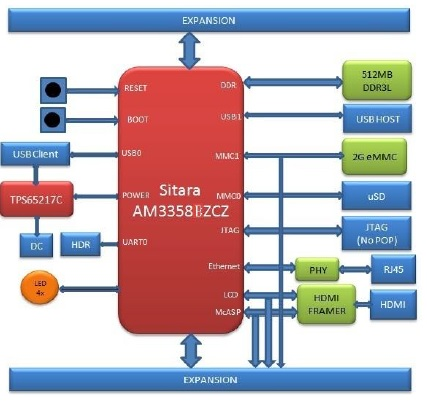
\includegraphics[scale=0.80]{./Resources/bbb-blockDG.jpg}
	\captionsetup{justification=centering}
	\caption[Diagrama de blocos de alto n�vel da BeagleBone Black]{Diagrama de blocos de alto n�vel da BeagleBone Black. \\Fonte: COLEY (2014)
	}
	\label{bbb-bdg}
\end{figure}

Cada pino de GPIO digital da BBB possui at� 7 modos diferentes de opera��o, que s�o configurados utilizando uma ferramenta do Linux chamada \textit{Device Tree}. A figura \ref{bbb_pins_def} apresenta a configura��o padr�o dos pinos, ou seja, quando � usada a distribui��o Angstrom do Linux, pr�-compilada e que � fornecida com a placa. Com rela��o aos pinos de GPIO, � importante notar que sua l�gica opera com n�veis de tens�o de 0V e 3,3V para os n�veis baixo e alto, respectivamente e portanto aplicar uma tens�o negativa ou superior a 3,3V pode danificar permanentemente a placa \cite{lumme}.

\begin{figure}[H]
	\centering
	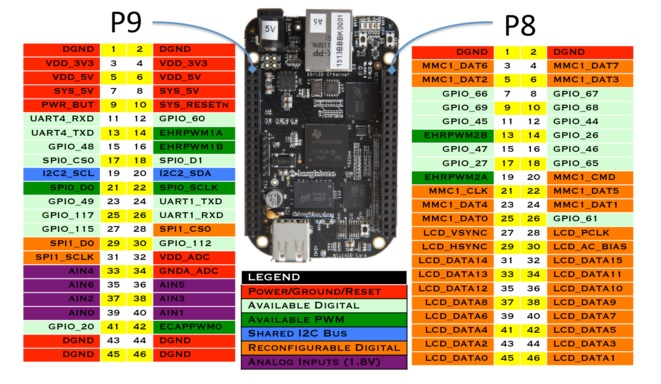
\includegraphics[scale=0.80]{./Resources/bbb-pins-def.jpg}
	\captionsetup{justification=centering}
	\caption[Configura��o padr�o dos pinos da BeagleBone Black]{Configura��o padr�o dos pinos da BeagleBone Black. \\Fonte: Site oficial da Funda��o BeagleBoard.org\protect\footnotemark
	}
	\label{bbb_pins_def}
\end{figure}

\footnotetext{Dispon�vel em \url{http://beagleboard.org/Support/bone101}}

\subsection{\textit{Programmable Real-time Unit -- PRU-ICSS}}

A PRU-ICSS -- \textit{Programmable Real-Time Unit Subsystem and Industrial Communications Subsystem} (Unidade Program�vel de Tempo-Real e Subsistema de Comunica��o Industrial, em tradu��o livre) � um subsistema do processador AM3358 que equipa a BBB, que � fabricado pela \textit{Texas Instruments} mas n�o tem suporte oficial da mesma \cite{bbb_srm}. Esta unidade consiste de dois n�cleos RISC de 32 bits, uma mem�ria compartilhada de 12kB, uma mem�ria de dados e uma mem�ria de programa para cada n�cleo, ambas com 8kB de capacidade e perif�ricos internos -- al�m da possibilidade de acessar todos os eventos, pinos e recursos do SoC AM3358 por meio de uma interface OCP, que confere a este subsistema grande flexibilidade. Cada n�cleo da PRU pode operar independentemente ou de maneira sincronizada, dependendo de como o \textit{firmware} para eles � escrito \cite{soc_manual}. Na figura � ilustrado o diagrama de blocos deste sistema.

\begin{figure}[H]
	\centering
	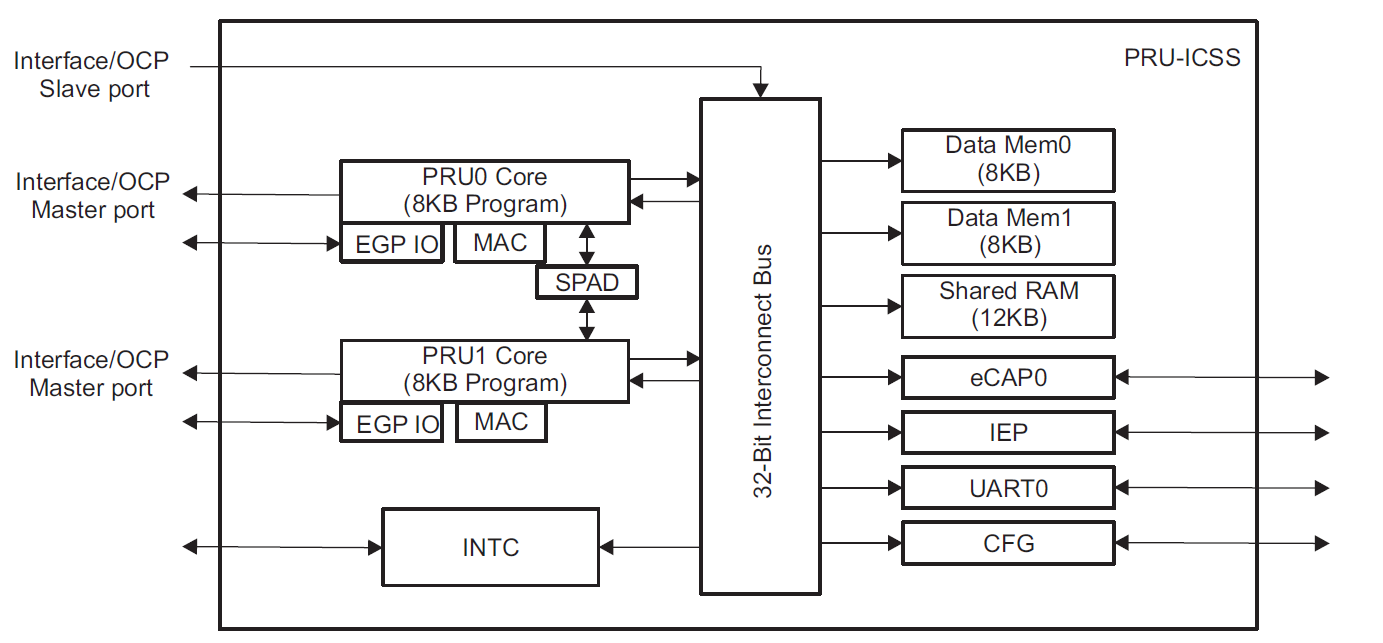
\includegraphics[scale=0.40]{./Resources/pru-blockDG.png}
	\captionsetup{justification=centering}
	\caption[Diagrama de blocos do subsistema PRU-ICSS]{Diagrama de blocos do subsistema PRU-ICSS. \\Fonte: TEXAS INSTRUMENTS (2015)
	}
	\label{pru-bdg}
\end{figure}

Os n�cleos da PRU foram otimizados para realizar tarefas com requisitos severos de tempo-real e, portanto, tem um \textit{clock} de 200MHz e um sistema de instru��es RISC no qual todas elas s�o executadas em um ciclo de \textit{clock}, propositalmente sem suporte a \textit{pipelining}. Cada n�cleo tem 31 registradores, cuja utiliza��o vai de prop�sito geral a indexa��o e controle de GPIO, acess�veis a n�vel de bit, byte, \textit{halfword} (16 bits), \textit{word} (32 bits) ou por ponteiro \cite{soc_manual}. Uma vez que cada instru��o pode ser executada em 5ns e o acesso a GPIO � feito por meio de uma �nica instru��o de acesso a registradores, isto significa que � poss�vel obter uma resolu��o de chaveamento determin�stica de no m�ximo 5ns, com dados obtidos na pr�tica, por \cite{bbb_pulsegen}, de \textit{jitter} RMS de 290ps e estabilidade de frequ�ncia na ordem de 10 ppm .

Uma vez que as diversas funcionalidades do m�dulo PRU s�o acessadas por meio de mapeamento da mem�ria de dados, � preciso saber a faixa de endere�o destas. Aqui deve ser feita a distin��o entre acesso � mem�ria local da PRU, que compreende os endere�os de 0x0000\_0000 a 0x0007\_FFFF, e o acesso � mem�ria global, cujos endere�os come�am em 0x0008\_0000. Tamb�m � importante notar que as mem�rias internas dos m�dulos podem ser acessados com o endere�o global de mem�ria, mas isso reduz significativamente o tempo de acesso, j� que o sinal � roteado para fora da PRU antes de ser recebido \cite{soc_manual}. Na tabela \ref{pru_localmem} � apresentado o mapa de mem�ria local e na tabela \ref{pru_globalmem} � apresentado o mapa de mem�ria global. Tamb�m h� uma tabela de constantes gravada em hardware, com valores de uso recorrente, para economizar instru��es de programa��o e registradores, nos quais estes endere�os precisariam ser carregados se n�o estivessem dispon�veis em hardware \cite{soc_manual}.

Embora cada PRU suporte 30 canais de entrada e 32 canais de sa�da no modo direto \cite{soc_manual}, a BBB roteia somente 25 pinos do SoC ao conector de expans�o. Destes, 10 pinos s�o exclusivos da PRU0 (8 sa�das ou 9 entradas) e 15 pinos para a PRU1 (13 sa�das ou 14 entradas). Eventualmente, alguns pinos pr�-configurados para outras fun��es devem ser reconfigurados antes que possam ser utilizados \cite{bbb_srm}. Os pinos da BBB acess�veis pela PRU podem ser obtidos na figura \ref{bbb_pins_pru}.

\begin{figure}[H]
	\centering
	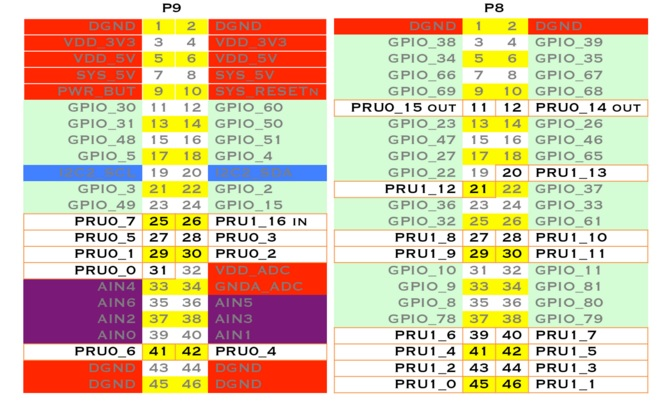
\includegraphics[scale=0.80]{./Resources/bbb-pins-pru.jpg}
	\captionsetup{justification=centering}
	\caption[Pinos da BeagleBone Black acess�veis pela PRU-ICSS]{Pinos da BeagleBone Black acess�veis pela PRU-ICSS. \\Fonte: Site oficial da Funda��o BeagleBoard.org\protect\footnotemark
	}
	\label{bbb_pins_pru}
\end{figure}

\footnotetext{Dispon�vel em \url{http://beagleboard.org/Support/bone101}}

\begin{center}
	\begin{table}[H]
		\captionsetup{justification=centering}
		\caption[Mapa de Mem�ria Local da PRU]{Mapa de Mem�ria Local da PRU. \\Fonte: adaptado de TEXAS INSTRUMENTS(2014)}
		\label{pru_localmem}
		\begin{tabular}{ | M{5cm} | M{5cm} | M{5cm} |}
			\hline
			\textbf{Endere�o Inicial} & \textbf{PRU0} & \textbf{PRU1} \\ \hline
			0x0000\_0000 & Mem. dados da PRU0 & Mem. dados da PRU1\\ \hline
			0x0000\_2000 & Mem. dados da PRU1 & Mem. dados da PRU0\\ \hline
			0x0001\_0000 & Mem. dados compartilhada & Mem. dados compartilhada \\ \hline
			0x0002\_0000 & INTC & INTC \\ \hline
			0x0002\_2000 & Controle da PRU0 & Controle da PRU0 \\ \hline
			0x0002\_2400 & Reservado & Reservado \\ \hline
			0x0002\_4000 & Controle da PRU1 & Controle da PRU1 \\ \hline
			0x0002\_4400 & Reservado & Reservado \\ \hline
			0x0002\_6000 & CFG & CFG \\ \hline
			0x0002\_8000 & UART0 & UART0 \\ \hline
			0x0002\_A000 & Reservado & Reservado \\ \hline
			0x0002\_C000 & Reservado & Reservado \\ \hline
			0x0002\_E000 & IEP & IEP \\ \hline
			0x0003\_0000 & eCAP0 & eCAP0 \\ \hline
			0x0003\_2000 & Reservado & Reservado \\ \hline
			0x0003\_2400 & Reservado & Reservado  \\ \hline
			0x0003\_4000 & Reservado & Reservado  \\ \hline
			0x0003\_8000 & Reservado & Reservado  \\ \hline
			0x0004\_0000 & Reservado & Reservado  \\ \hline
			0x0008\_0000 & System OCP\_HP0 & System OCP\_HP1 \\ \hline
		\end{tabular}
	\end{table}
\end{center}

As interfaces de interrup��o e de GPIO est�o contidas nos registradores R30 e R31: o registrador R31 � utilizado tanto para interface dos pinos configurados como entrada quanto para leitura e/ou gera��o de eventos de interrup��o, enquanto o registrador R30
retorna status ou muda o valor dos pinos configurados como sa�da, para leitura e escrita, respectivamente. Embora a entrada possa ser configurada nos modos de captura paralela de 16 bits e trem de pulsos de 28 bits, estes modos de opera��o n�o ser�o detalhados, j� que seu uso n�o est� contido no escopo deste projeto. O mesmo � v�lido para a sa�da, que al�m do modo direto, pode ser configurada para transmitir um trem de pulsos \cite{soc_manual}.

Outra caracter�stica da PRU � a exist�ncia de um IEP - \textit{Industrial Ethernet Peripheral} (Perif�rico Ethernet Industrial, em tradu��o livre), composto de um \textit{timer} para Ethernet industrial com 8 eventos de compara��o e uma porta digital de E/S. O \textit{timer} Ethernet industrial � simplesmente um temporizador de 32 bits e, portanto, pode ser utilizado para uso geral. � um contador positivo, cujo valor dos incrementos pode ser programado na faixa de 1-16, com compensador de uso opcional. Os 8 registradores comparadores permitem a cria��o de eventos cada vez que o valor do comparador corresponde ao do temporizador \cite{soc_manual}.

\begin{center}
	\begin{table}[H]
		\captionsetup{justification=centering}
		\caption[Mapa de Mem�ria Global da PRU]{Mapa de Mem�ria Global da PRU. \\Fonte: adaptado de TEXAS INSTRUMENTS(2014)}
		\label{pru_globalmem}
		\begin{tabular}{ | M{5cm} | M{10cm} |}
			\hline
			\textbf{Endere�o de Offset} & PRU-ICSS \\ \hline
			0x0000\_0000 & Mem. dados da PRU0 \\ \hline
			0x0000\_2000 & Mem. dados da PRU1 \\ \hline
			0x0001\_0000 & Mem. dados compartilhada \\ \hline
			0x0002\_0000 & INTC \\ \hline
			0x0002\_2000 & Controle da PRU0 \\ \hline
			0x0002\_2400 & Debug da PRU0 \\ \hline
			0x0002\_4000 & Controle da PRU1 \\ \hline
			0x0002\_4400 & Debug da PRU1 \\ \hline
			0x0002\_6000 & CFG \\ \hline
			0x0002\_8000 & UART0 \\ \hline
			0x0002\_A000 & Reservado \\ \hline
			0x0002\_C000 & Reservado \\ \hline
			0x0002\_E000 & IEP \\ \hline
			0x0003\_0000 & eCAP0 \\ \hline
			0x0003\_2000 & Reservado \\ \hline
			0x0003\_2400 & Reservado  \\ \hline
			0x0003\_4000 & IRAM da PRU0  \\ \hline
			0x0003\_8000 & IRAM da PRU1  \\ \hline
			0x0004\_0000 & Reservado  \\ \hline
		\end{tabular}
	\end{table}
\end{center}

No que diz respeito ao desenvolvimento de \textit{firmware} para a PRU, h� um conjunto de instru��es RISC em assembly, suportado por um conjunto de ferramentas que ajudam a gerar o arquivo bin�rio a ser carregado na mem�ria de programa. Alguns exemplos s�o o \textit{assembler}, \textit{archiver} e o \textit{linker} \cite{pru_assembly_tools}. Outra ferramenta de desenvolvimento proporcionada pela Texas Instruments � um compilador C/C++, que facilita a programa��o em n�veis de abstra��o elevados \cite{pru_compiler}. A figura \ref{pru_firmdev} apresenta um diagrama de blocos que ilustra os passos a serem executados desde compilar o c�digo C/C++ at� carregar o arquivo execut�vel na mem�ria de programa da PRU.

\begin{figure}[H]
	\centering
	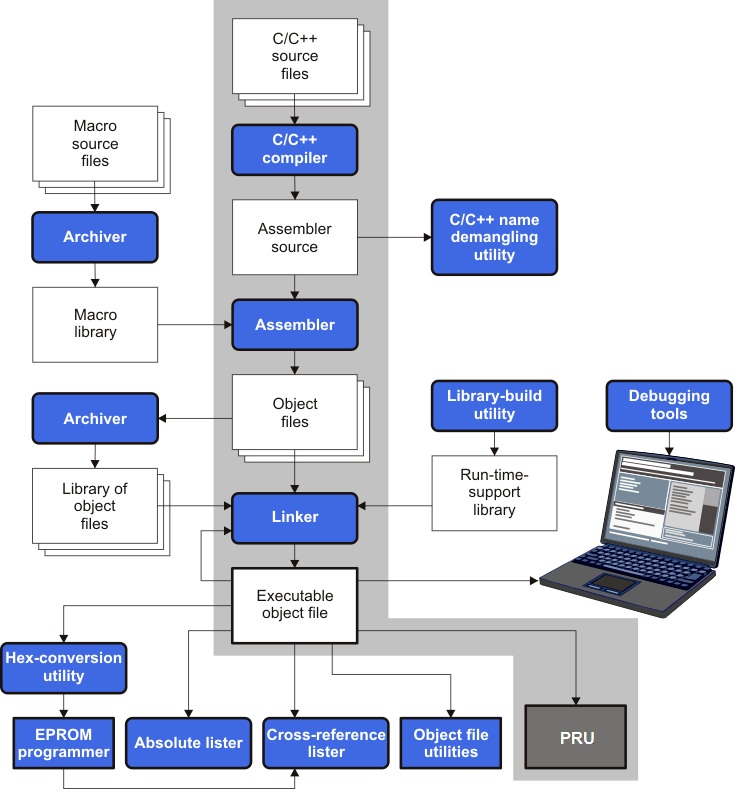
\includegraphics[scale=0.80]{./Resources/pru-software-dev.png}
	\captionsetup{justification=centering}
	\caption[Fluxo de desenvolvimento de software da PRU]{Fluxo de desenvolvimento de software da PRU. \\Fonte: TEXAS INSTRUMENTS
	}
	\label{pru_firmdev}
\end{figure}

\subsection{\textit{Device Tree}}

A \textit{Device Tree} ou DT � basicamente uma estrutura de dados utilizada para descrever \textit{hardware}, cujo objetivo � possibilitar que as caracter�sticas de \textit{hardware} de um sistema espec�fico sejam passadas para o SO durante o \textit{boot}, ao inv�s de estas informa��es ficarem gravadas no SO \cite{devicetree}, o que possibilita que um \textit{driver} do Kernel seja usado em configura��es diferentes de \textit{hardware} sem a necessidade de modifica��es em seu c�digo-fonte. Com rela��o aos sistemas equipados com processadores ARM, a necessidade de uso da DT surgiu devido ao grande n�mero de novas placas, que tornou muito dif�cil manter uma vers�o do Kernel para cada sistema. Seu objetivo n�o � modificar o sistema em tempo de execu��o, por�m no caso da BBB, foi criada uma solu��o chamada \textit{Device Tree Overlay} (ou sobreposi��o) para executar esta fun��o, facilitando a configura��o de GPIO, dentre outras fun��es, e uso da DT pelo usu�rio final \cite{bbb_devicetree}, fatores que s�o do interesse de aprendizes da �rea.

Uma DT � uma estrutura em �rvore, composta de n�s e propriedades. Uma abordagem para entender o seu funcionamento � por meio de um exemplo de sobreposi��o espec�fico para a BBB. Abaixo � apresentado um exemplo de sobreposi��o de DT espec�fico da BBB que apresenta os principais conceitos para o uso desta ferramenta:

\newpage

\lstset{language=dtc}
\begin{lstlisting}[frame=single, basicstyle=\linespread{0.85}\ttfamily]

/*
* Copyright (C) 2013 CircuitCo
*
* Virtual cape for UART1 on connector pins P9.24 P9.26
*
* This program is free software; you can redistribute it and/or modify
* it under the terms of the GNU General Public License version 2 as
* published by the Free Software Foundation.
*/
/dts-v1/;
/plugin/;

/ {
	compatible = "ti,beaglebone", "ti,beaglebone-black";

	/* identification */
	part-number = "BB-UART1";
	version = "00A0";
	
	/* state the resources this cape uses */
	exclusive-use =
		/* the pin header uses */
		"P9.24",        /* uart1_txd */
		"P9.26",        /* uart1_rxd */
		/* the hardware ip uses */
		"uart1";
	
	fragment@0 {
		target = <&am33xx_pinmux>;
		__overlay__ {
			bb_uart1_pins: pinmux_bb_uart1_pins {
				pinctrl-single,pins = <
		/* P9.24 uart1_txd.uart1_txd MODE0 OUTPUT (TX) */
					0x184 0x20
		/* P9.26 uart1_rxd.uart1_rxd MODE0 INPUT (RX) */ 
					0x180 0x20
				>;
			};
		};
	};
	
	fragment@1 {
		target = <&uart2>;	/* really uart1 */
		__overlay__ {
			status = "okay";
			pinctrl-names = "default";
			pinctrl-0 = <&bb_uart1_pins>;
		};
	};
};
\end{lstlisting}

Neste c�digo, na linha 14 � definida a plataforma � qual esta DT se refere. Com isso, ficam declaradas as funcionalidades de \textit{hardware} do sistema. Na sequ�ncia, a identifica��o mostra quais sobreposi��es de DT est�o carregadas e o nome do arquivo compilado deve ser igual ao nome nela atribu�do; a vers�o deve ser 00A0 para a BBB. Entre as linhas 20 e 26 s�o listados os recursos de \textit{hardware} utilizados por esta sobreposi��o, que impedem que outras sobreposi��es que usem os mesmos recursos sejam carregadas; no caso deste exemplo, os pinos referentes � UART1, assim como o pr�prio dispositivo UART1 s�o utilizados. A seguir, os fragmentos descrevem qual dispositivo ter� suas configura��es sobrepostas. No fragmento 0, � o multiplexador dos pinos da BBB, compat�vel com o \textit{driver} \textit{pinctrl-single} - os dois valores hexadecimais utilizados para cada pino s�o o \textit{offset} do pino com rela��o ao seu registrador e a configura��o do pino. J� no fragmento 1 � configurada a interface UART1. Por enquanto, ser�o introduzidas somente as quest�es referentes � configura��o do multiplexador, uma vez que seu conhecimento � necess�rio para o uso dos pinos no modo GPIO.

Para determinar o valor hexadecimal de \textit{offset} do pino ao qual se deseja aplicar uma configura��o, primeiro � preciso obter seu nome a partir do seu n�mero na barra de pinos, conforme ilustrado na figura \ref{bbb_pins_def}, consultando as tabelas \ref{p8-header} e \ref{p9-header}, nas quais o nome do pino � referente ao \textbf{modo 0}, que tamb�m � o nome do pino no manual do SoC \cite{bbb_srm, soc_manual}. A seguir, obt�m-se o valor hexadecimal do registrador referente ao pino, na tabela \ref{dt_offset} presente no anexo \ref{Anexo2}, adaptada do manual do SoC, e subtrai-se 0x800 de seu valor original.

Com rela��o � configura��o do pino, este aceita os par�metros de ajuste de \textit{slew-rate}, ativa��o do \textit{buffer} de entrada, ajuste e ativa��o do \textit{pull-up/pull-down} interno e sele��o do modo de opera��o do pino. Note-se que, com rela��o ao buffer de entrada, ao menos um blog da internet refere-se a este bit como sendo um bit de sele��o para entrada \textbf{ou} sa�da \cite{derek_devtree}, por�m o manual indica que quando o bit est� setado, o pino pode ser usado tanto como entrada quanto sa�da \cite{soc_manual}. A tabela \ref{pad_cfg} apresenta os campos do registrador de controle de E/S, assim como a descri��o de cada campo e os valores aceitos.

\begin{center}
	\begin{table}[H]
		\captionsetup{justification=centering}
		\caption[Descri��o dos campos do registrador de controle de \textit{pads}]{Descri��o dos campos do registrador de controle de \textit{pads}. \\Fonte: adaptado de TEXAS INSTRUMENTS(2014)}
		\label{pad_cfg}
		\begin{tabular}{ | M{1cm} | M{3cm} | M{1cm} | M{10cm} |}
			\hline
			\textbf{Bit} & \textbf{Campo} & \textbf{Valor} & \textbf{Descri��o} \\ \hline
			31-7 & Reservado &  & Reservado. Leitura retorna 0 \\ \hline
			6 & SLEWCTRL & \shortstack{ \quad \\ 0 \\ 1} & \shortstack{Seleciona entre \textit{slew-rate} r�pido ou lento \\ 0 - r�pido \\ 1 - lento} \\ \hline
			5 & RXACTIVE & \shortstack{ \quad \\ 0 \\ 1} & \shortstack{Ativa modo de entrada para o pino \\ 0 - somente sa�da \\ 1 - Receptor ativado. Entrada ou sa�da}. \\ \hline
			4 & PULLTYPESEL & \shortstack{ \quad \\ 0 \\ 1} & \shortstack{Sele��o de pull-up/pull-down \\ 0 - pull-down \\ 1 - pull-up} \\ \hline
			3 & PULLUDEN & \shortstack{ \quad \\ 0 \\ 1} & \shortstack{Habilita pull-up/pull-down \\ 0 - habilitado \\ 1 - desabilitado} \\ \hline
			2-0 & MUXMODE & 0-7 & Sele��o de funcionalidade do pino multiplexado \\ \hline
		\end{tabular}
	\end{table}
\end{center}

\newpage

%tabela do header 8
\begin{minipage}[t][.49\textheight]{1\textwidth}
	\begin{center}
		\begin{table}[H]
			\captionsetup{justification=centering}
			\caption[Lista de pinos do \textit{header} P8 e seus respectivos modos de funcionamento]{Lista de pinos do \textit{header} P8 e seus respectivos modos de funcionamento \\ fonte: COLEY}
			\label{p8-header}
			\begin{center}
				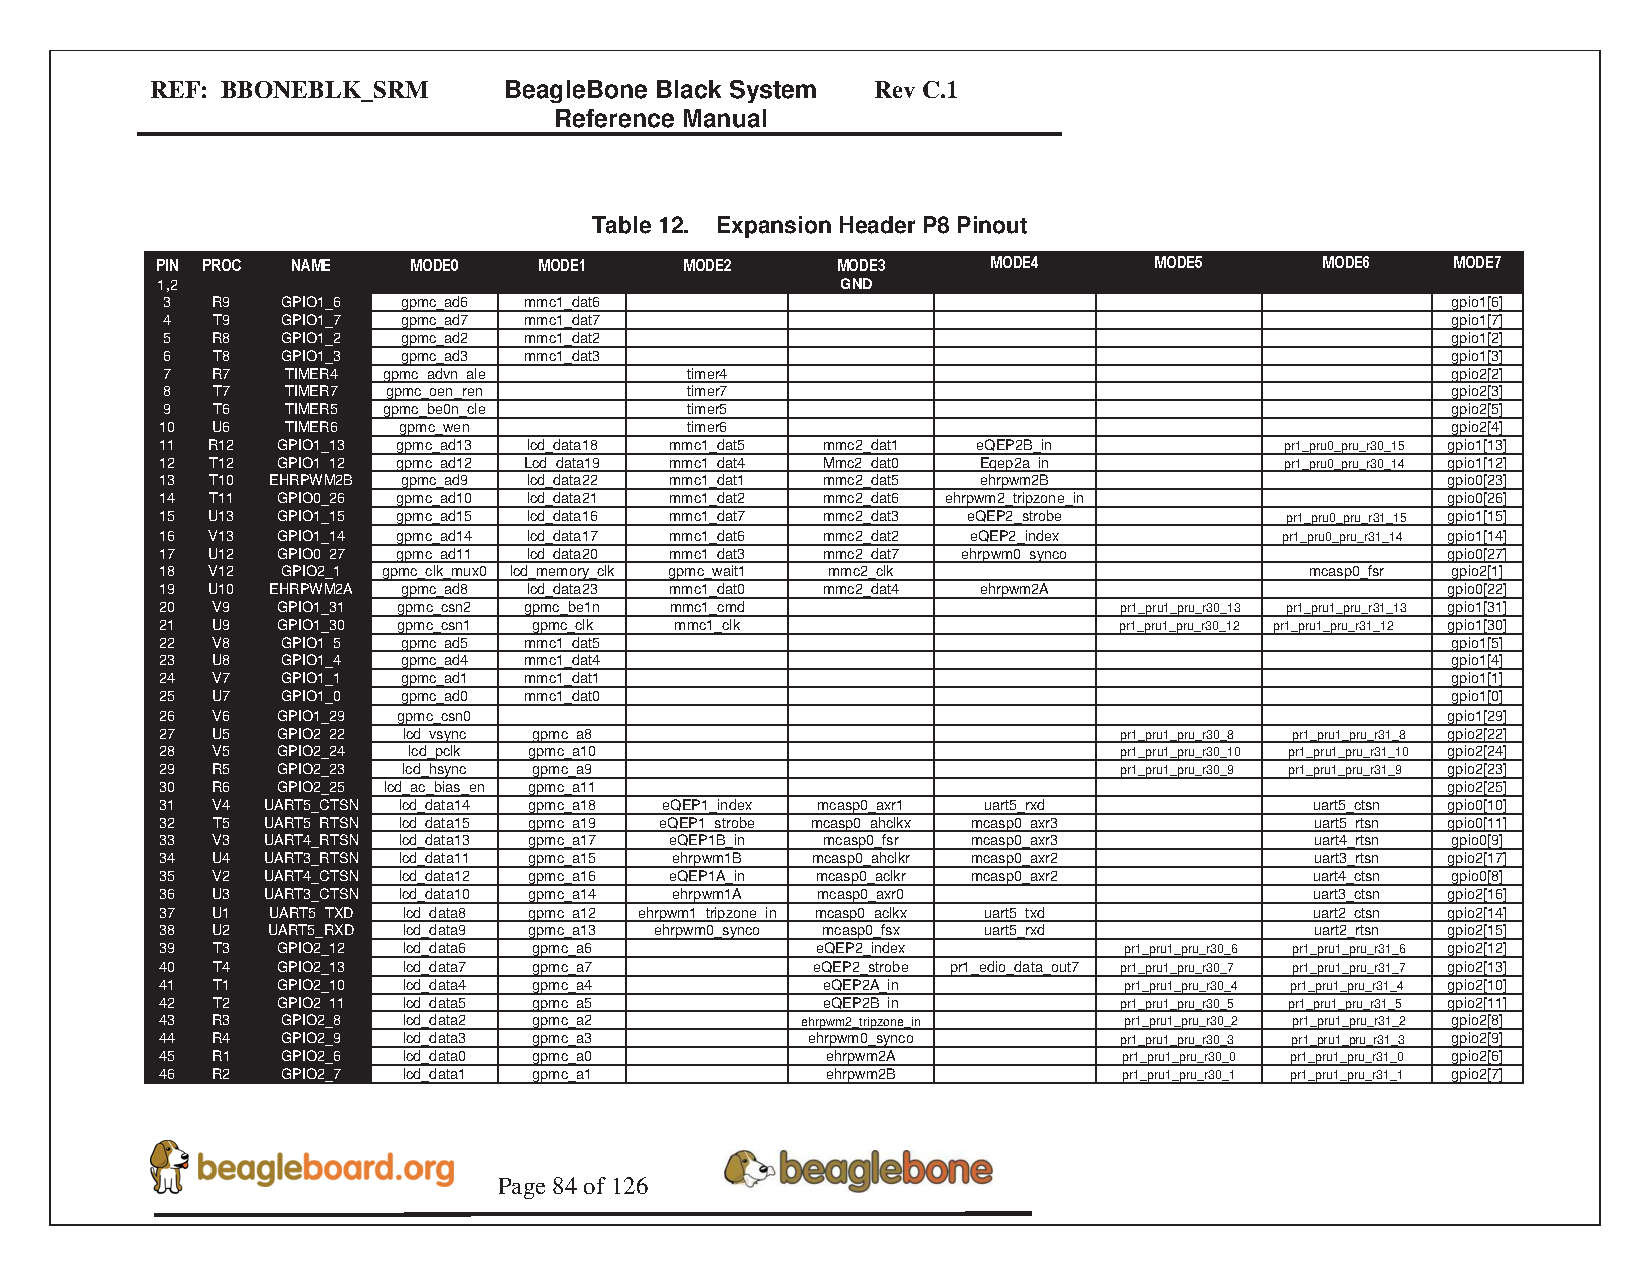
\includegraphics[page=1, height=0.4\textheight]{./Resources/tabela_pinos_SRM.pdf}
			\end{center}
		\end{table}
		%\includegraphics[page=3, scale=0.5]{./Resources/BBB_SCH.pdf}
	\end{center}
\end{minipage}

%tabela do header 9
\begin{minipage}[b][.49\textheight]{1\textwidth}
	\begin{center}
		\begin{table}[H]
			\captionsetup{justification=centering}
			\caption[Lista de pinos do \textit{header} P9 e seus respectivos modos de funcionamento]{Lista de pinos do \textit{header} P9 e seus respectivos modos de funcionamento \\ fonte: COLEY}
			\label{p9-header}
			\begin{center}
				\includegraphics[page=2, height=0.4\textheight]{./Resources/tabela_pinos_SRM.pdf}
			\end{center}
		\end{table}
		%\includegraphics[page=3, scale=0.5]{./Resources/BBB_SCH.pdf}
	\end{center}
\end{minipage}

%P�ginas relevantes do manual do SoC
%1356 - pullup, RXactive, etc e 1365 - registers offset, 1422 - registrador

%\subsection{Programa��o em Python}

\section{Programa��o em Node.js (Javascript)}

Node.js � um ambiente em tempo de execu��o recente, criado em 2009 \cite{node_created},que permite a execu��o no servidor de programas escritos em Javascript. Para tal, este ambiente utiliza um motor implementado pelo Google para seu navegador Chrome --- o \textit{V8}, que compila o Javascript em c�digo de m�quina e n�o \textit{bytecode} ou interpreta��o \textit{on-the-fly}, o que torna a execu��o de Javascript extremamente r�pida \cite{node_fast}, embora seja importante lembrar que o \textit{overhead} inerente de lingaugens de tipagem din�mica custa o tempo de processamento de resolu��o do tipo de vari�vel utilizada \cite{node_dyntype}. 

Node, devido � natureza ass�ncrona de I/O do Javascript, implementa um suporte nativo � programa��o orientada a eventos, ainda que seja executado em uma �nica \textit{thread}, o que o torna um diferencial com rela��o �s outras lingaugens de programa��o mais populares, que exigem do desenvolvedor a implementa��o de processos de \textit{multithreading} para atingir paralelismo de processamento \cite{node_intro}. Ainda, o estilo de programa��o em Node � orientado a \textit{callbacks}, que nada mais � do que passar como argumento uma fun��o que ser� executada assim que um evento acabar.

Historicamente, o desenvolvimento de \textit{multithreading} surgiu da necessidade de servi�os de rede que possibilitassem m�ltiplas comunica��es em paralelo, o que � conhecido como m�ltiplas fontes de I/O e assim ser� referenciado neste trabalho --- isto ocorreu devido ao fato de linguagens tradicionais de programa��o, mais antigas, focarem na implementa��o de aplica��es operadas por um �nico ser humano enquanto, com o desenvolvimento da internet, esta realidade mudou drasticamente, exigindo processamento de I/O massivo \cite{node_book}. Em processadores com diversos n�cleos, isso significa processamento em paralelo, enquanto em processadores com um �nico n�cleo � implementada uma multiplexa��o temporal que permite tal t�cnica. O fato mais not�vel das implementa��es de \textit{multithreading} � a complexidade do c�digo, que n�o � trivial e geralmente d� origem a c�digos mal estruturados e repletos de vari�veis globais, dif�ceis de manter \cite{node_intro, node_book}.

Javascript, que nasceu como uma linguagem para execu��o no cliente, tornou-se a espinha dorsal de aplica��es HTML modernas e, recentemente, ficou muito popular dentre aplica��es no servidor. Especificamente em Node, o comportamento ass�ncrono � a regra geral, devido � orienta��o a eventos. Isto leva programadores acostumados a linguagens s�ncronas como C a terem dificuldades iniciais de programa��o: o uso de \textit{callbacks} de evento � fundamental para estruturar a ordem com que certas tarefas s�o executadas, sempre ap�s o final do evento pai \cite{node_book}. � importante salientar que este tipo de implementa��o ocorre de forma transparente ao usu�rio mas, na verdade, nada mais � do que um \textit{loop} principal cujo objetivo � cuidar de todas as chamadas a fun��es. Outro ponto not�vel relacionado ao Node � que, para executar aplica��es em m�ltiplos n�cleos, � preciso executar m�ltiplas inst�ncias, o que pode ser gerenciado com bibliotecas de suporte \cite{node_intro, node_book}. Note-se tamb�m que os termos \textit{orientado a eventos} e \textit{ass�ncrono} s�o equivalentes \cite{node_book}.

Para ilustrar o comportamento ass�ncrono do Node, no c�digo a seguir n�o h� garantia alguma de que a fun��o executada na segunda linha receba um par�metro diferente de nulo (Null) \cite{node_book}:

\lstset{language=javascript}
\begin{lstlisting}[frame=single, basicstyle=\linespread{0.85}\ttfamily]
var botaoStatus = leBotao();
imprimeValorBotao(botaoStatus); //nao ha garantia de que leBotao ja acabou de ser executada
\end{lstlisting}

A maneira correta para executar este tipo de c�digo seria usando uma fun��o de callback, como descrito no trecho de c�digo abaixo, embora esta n�o seja a �nica maneira de faz�-lo. Observe-se que a fun��o � declarada como um par�metro de \textit{leBotao} e n�o tem nome --- � uma fun��o an�nima. Embora isto seja pr�tico, do ponto de vista de manuten��o de c�digo e \textit{debug} � uma pr�tica que deve ser evitada \cite{callback_hell, avoid_hell}.

\lstset{language=javascript}
\begin{lstlisting}[frame=single, basicstyle=\linespread{0.85}\ttfamily]
leBotao(function(botaoStatus){
	imprimeValorBotao(botaoStatus); //so acontece depois que o botao eh lido
});
\end{lstlisting}

\subsection{\textit{Node Package Manager - NPM}}

O \textit{Node Package Manager}, ou simplesmente NPM, � n�o somente um gerenciador de pacotes como tamb�m � um reposit�rio de pacotes de terceiros e um padr�o para defini��o de depend�ncias. Os pacotes ficam em um registro p�blico e podem ser gerenciados por uma ferramenta pr�pria por linha de comando. O uso do NPM n�o � obrigat�rio, mas � medida que aplica��es mais complexas s�o desenvolvidas � quase mandat�rio seu uso, pois assim � poss�vel usar m�dulos prontos para executar diversas tarefas com facilidade. Uma vantagem do NPM � que os m�dulos podem ser instalados localmente, restringindo-os ao diret�rio do projeto e, portanto, garantindo certo n�vel de seguran�a. \cite{node_book}. Abaixo � apresentado um exemplo no qual o pacote fict�cio \textit{meuPacote} � instalado para a vers�o mais recente adicionada ao reposit�rio do NPM:

\lstset{language=bash}
\begin{lstlisting}[frame=single, basicstyle=\linespread{0.85}\ttfamily]
npm install meuPacote@latest
\end{lstlisting}

Outro exemplo de uso do NPM � a defini��o de depend�ncias de um projeto e posterior possibilidade de instala��o de todas elas de uma s� vez. Para isto, um arquivo no formato JSON descreve estas depend�ncias e outras informa��es do projeto:

\lstset{language=javascript}
\begin{lstlisting}[frame=single, basicstyle=\linespread{0.85}\ttfamily]
{
	"name" : "meuPacote",
	"version" : "1.0.0",
	"dependencies" : {
		"debug" : "0.3.x",
		"nano" : "*",
		"request" : ">0.2.0"
	}
}
\end{lstlisting}

E a instala��o das depend�ncias se d� da seguinte maneira, assumindo que o presente diret�rio de trabalho � o mesmo do projeto:

\lstset{language=bash}
\begin{lstlisting}[frame=single, basicstyle=\linespread{0.85}\ttfamily]
npm install
\end{lstlisting}

\subsection{\textit{MEAN Stack}}

MEAN � uma pilha de desenvolvimento, de c�digo aberto, para aplica��es web e prov� um conjunto de quatro ferramentas que, juntas, s�o a base necess�ria para a cria��o de aplica��es tanto de servidor quanto do cliente. Um exemplo de pilha de desenvolvimento para aplica��es web muito disseminado � a pilha LAMP. Voltando � MEAN, cada uma das 4 letras deste acr�nimo representa uma das ferramentas \cite{node_mean}:

\begin{itemize}
	\item \textbf{MongoDB} - banco de dados orientado a objetos
	\item \textbf{Express.js} - framework para cria��o de servidor web e roteamento
	\item \textbf{Angular.js} - framework para aplica��es web
	\item \textbf{Node.js} - base da aplica��o do servidor
\end{itemize}

Note-se que toda a pilha � baseada na linguagem Javascript, o que permite ao desenvolvedor de uma solu��o completa uma curva de aprendizado mais r�pida, pois menos tempo � empregado aprendendo a sintaxe e o paradigma de programa��o e mais tempo dedicado � funcionalidade da aplica��o em si \cite{node_mean}.

\subsection{Servidor Express.js}

Express � um framework de \textit{middleware} para implementa��o de aplica��es web no servidor, incluindo mas n�o limitado a roteamento e opera��es HTTP, a exemplo dos m�todos GET e POST. Embora o Node apresente um m�dulo dedicado a HTTP, a proposta do Express � simplificar seu uso e evitar que o mesmo trabalho seja realizado m�ltiplas vezes e por v�rias pessoas diferentes \cite{node_mean}.

Dentre as facilidades proporcionadas pelo node est� a f�cil implementa��o de diferentes respostas para diferentes tipos de requisi��es baseadas no m�todo HTTP e a renderiza��o din�mica de documentos HTML \cite{node_book}. O tratamento de requisi��es baseadas no m�todo HTTP, possibilitado pelo Express, tamb�m � conhecido como RESTful API, que � uma API baseada no REST (\textit{Representational State Transfer}). Este por sua vez � um modelo para servi�os web que implementa as opera��es HTTP POST, GET, PUT e DELETE, que s�o mapeadas como opera��es b�sicas de banco de dados: criar, ler, atualizar e deletar \cite{node_mean}.

%\subsection{Performance do Node.js}

%\subsection{Intera��o com c�digo escrito em C/C++}

%\subsection{Confiabilidade e seguran�a quanto ao uso de m�dulos de terceiros}

%\section{Computa��o em nuvem e Internet das Coisas}

\section{Circuitos de Interface}

No �mbito deste trabalho, circuitos de interface s�o circuitos eletr�nicos que possibilitam a intera��o entre a plataforma BeagleBone Black e os sensores e atuadores do sistema mec�nico. O projeto adequado destes circuitos � essencial n�o somente para que o projeto funcione corretamente, mas tamb�m para evitar que componentes do sistema, a exemplo da BBB, sejam danificados. Nesta se��o, ser� abordada a teoria essencial para o projeto destes, desde conceitos relacionados � teoria de sinais, passando por alguns elementos b�sicos da eletr�nica e finalizando com as caracter�sticas dos sensores e atuadores empregados.

\subsection{Sinais}

Sinais s�o fun��es matem�ticas que guardam informa��es acerca de fen�menos f�sicos, a exemplo da temperatura de um elemento em fun��o do tempo ou a representa��o do som de um instrumento musical. Na figura \ref{seno_1p} � apresentado um per�odo de um sinal senoidal puro. Uma vez que, para obter informa��es a partir de um sinal, � preciso process�-lo, as mais diversas grandezas f�sicas devem ser convertidas para grandezas manipul�veis pelo sistema de processamento --- que no caso de circuitos eletr�nicos � comumente a tens�o el�trica, embora outras grandezas tamb�m sejam utilizadas \cite{sedra}. Para que a convers�o de diferentes grandezas f�sicas em sinais el�tricos seja poss�vel, s�o empregados dispositivos sensores e transdutores.

\begin{figure}[H]
	\centering
	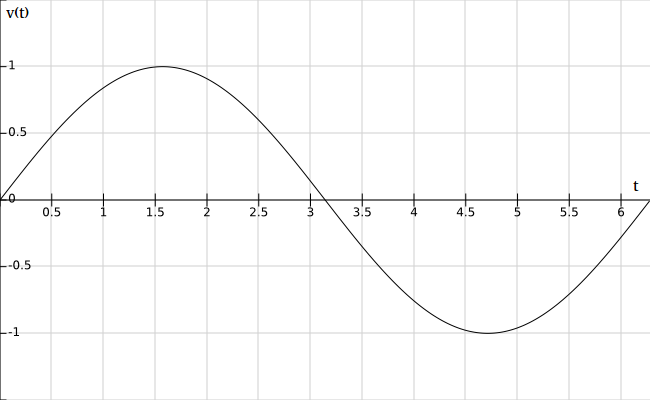
\includegraphics[scale=0.50]{./Resources/seno2.png}
	\captionsetup{justification=centering}
	\caption[Sinal senoidal em fun��o do tempo]{Sinal senoidal em fun��o do tempo}
	\label{seno_1p}
\end{figure}

\subsection{Dispositivos Semicondutores}

Diodos s�o os elementos eletr�nicos mais simples, constitu�dos de dois terminais que est�o conectados a uma jun��o PN, ou seja, a uma jun��o formada pelo contato entre dois cristais semicondutores dopados com impurezas de polaridades opostas \cite{juncoes_vero}. O efeito pr�tico desta jun��o � a capacidade de retifica��o: quando uma DDP positiva � aplicada aos terminais do diodo conforme exposto na figura \ref{diode}, a corrente el�trica flui pelos terminais do dispositivo e diz-se que o diodo est� polarizado diretamente; caso a DDP aplicada seja invertida, a corrente el�trica deixa de fluir pelo dispositivo \cite{sedra}. Este pode ser considerado o diodo ideal, que � o modelo mais simplificado deste elemento e n�o leva em considera��o nenhuma caracter�stica real do mesmo.

\begin{figure}[H]
	\centering
	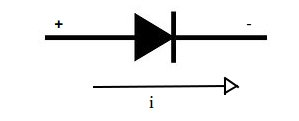
\includegraphics[scale=0.50]{./Resources/diode.jpg}
	\captionsetup{justification=centering}
	\caption[Representa��o esquem�tica do diodo polarizado diretamente]{Representa��o esquem�tica do diodo polarizado diretamente}
	\label{diode}
\end{figure}

O diodo ideal � descrito pela equa��o \ref{eq_diodo_real}, na qual $I_{s}$ � a corrente de satura��o reversa, $k=11600/\eta$, com $\eta$ igual a 1 para o germ�nio e 2 para o sil�cio e $T_{k}$ � a temperatura em kelvin. Muitas vezes, esta curva � aproximada por um modelo conhecido como \textit{circuito equivalente linear}, composto de um diodo em s�rie com uma fonte de tens�o e um resistor, que definem o limiar de condu��o e o n�vel de resist�ncia do dispositivo quando est� conduzindo \cite{boylestad}. A figura \ref{diodo_curva} ilustra um exemplo de defini��o do circuito equivalente a partir da representa��o real. Outra modelagem � conhecida como \textit{modelo para pequenos sinais}, no qual � fixado um ponto de opera��o em torno do qual a excurs�o do sinal aplicado ao circuito � pequena, conhecido como ponto de polariza��o ou \textbf{ponto quiescente}. Neste modelo, a regi�o exponencial � aproximada linearmente por um resistor cujo valor � o inverso da inclina��o da reta tangente ao ponto de polariza��o \cite{sedra}. Cabe salientar que o avan�o das ferramentas de computa��o tornaram poss�vel o c�lculo dos mais diversos circuitos eletr�nicos de forma r�pida e exata, relegando portanto os modelos simplificados a ferramentas de ensino ou para esbo�o de circuitos simples \cite{boylestad}, desde que os modelos empregados nas simula��es sejam fi�is ao comportamento real dos componentes \cite{sedra}.

\begin{equation}
	\label{eq_diodo_real}
	I_{d}=I_{s}\epsilon ^{kV_{d}/T_{k}}-I_{s}
\end{equation}

\begin{figure}[H]
	\centering
	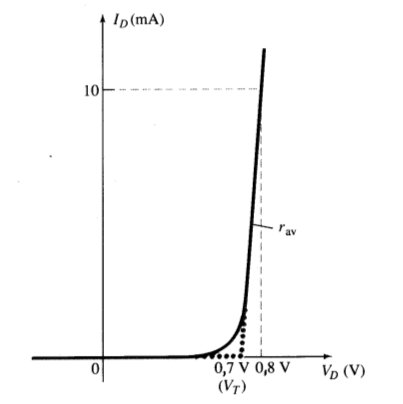
\includegraphics[scale=0.80]{./Resources/diodo_curva.jpg}
	\captionsetup{justification=centering}
	\caption[Defini��o do circuito equivalente linear, usando-se segmentos de reta para aproximar a curva caracter�stica]{Defini��o do circuito equivalente linear, usando-se segmentos de reta para aproximar a curva caracter�stica \\ Fonte: BOYLESTAD (2011)}
	\label{diodo_curva}
\end{figure}

A partir do conhecimento obtido com a introdu��o ao diodo e sua jun��o PN, ser� agora abordado o transistor bipolar de jun��o, tamb�m conhecido com BJT. De forma an�loga ao diodo, este dispositivo � constitu�do da jun��o de tr�s cristais semicondutores dopados, podendo ser uma jun��o do tipo NPN ou PNP: ambos funcionam de forma complementar, sendo que o tipo NPN conduz majoritariamente el�trons, enquanto o tipo PNP conduz majoritariamente lacunas. Na figura \ref{transistor} s�o apresentados os sentidos de corrente e os s�mbolos dos transistores PNP e NPN e, aplicando a lei das correntes de Kirchhoff, obt�m-se a rela��o entre as correntes de emissor, coletor e base do transistor, descritas pela equa��o \ref{eq_bjt_kirch} \cite{boylestad}. Note-se que � usado o sentido real da corrente e n�o o convencional, comumente adotado em c�lculos.

\begin{figure}[H]
	\centering
	\begin{subfigure}{.46\textwidth}
		\centering
		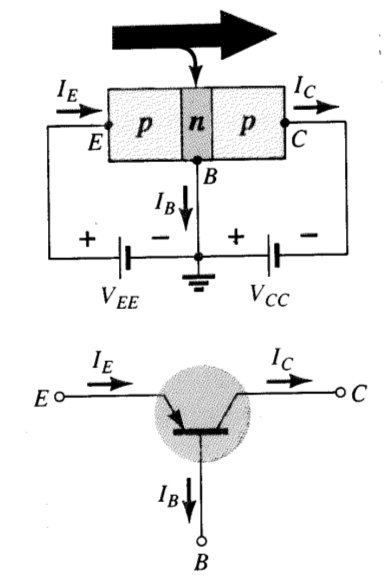
\includegraphics[height=8cm]{./Resources/bjt_pnp.jpg}
		\caption{Transistor \textit{pnp}}
		\label{transistor:1}
	\end{subfigure}
	\begin{subfigure}{.46\textwidth}
		\centering
		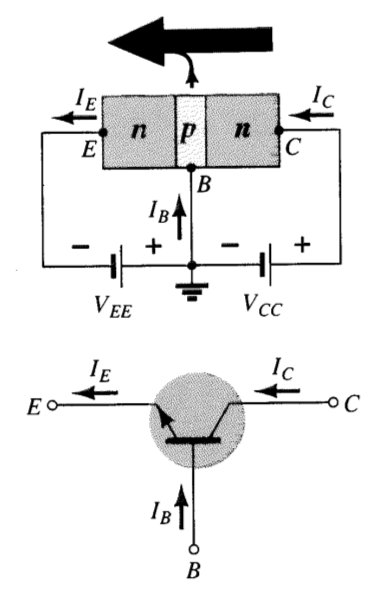
\includegraphics[height=8cm]{./Resources/bjt_npn.jpg}
		\caption{Transistor \textit{npn}}
		\label{transistor:2}
	\end{subfigure}
	\captionsetup{justification=centering}
	\caption[Nota��es e s�mbolos utilizados para a configura��o base-comum]{Nota��es e s�mbolos utilizados para a configura��o base-comum. \\Fonte: BOYLESTAD (2011)
	}
	\label{transistor}
\end{figure}

\begin{equation}
	\label{eq_bjt_kirch}
	I_{e}=I_{c} + I_{b}
\end{equation}

Para finalizar a introdu��o ao transistor bipolar, � apresentada uma rela��o simplificada entre as correntes de coletor $I_{c}$ e de base $I_{b}$ na equa��o \ref{eq_bjt_beta}, uma vez que esta � uma rela��o que permite a realiza��o de c�lculos r�pidos para esbo�ar circuitos com transistores BJT. Cabe salientar que a validade desta rela��o se d� somente quando o transistor est� corretamente polarizado e na regi�o de condu��o. Outro fato que deve ser levado em conta � que o valor de $\beta$ depende das caracter�sticas de constru��o de cada BJT e � um valor cujo desvio padr�o � elevado mesmo se comparados dois transistores reais do mesmo modelo \cite{boylestad}. Ainda que o conte�do relativo a transistores BJT seja muito mais extenso e detalhado, cabe ao leitor consultar as refer�ncias bilbiogr�ficas \cite{boylestad} e \cite{sedra} para mais detalhes acerca do tema. 

\begin{equation}
	\label{eq_bjt_beta}
	I_{c} = \beta\cdot I_{b}
\end{equation}

Existe outro tipo de transistor conhecido como transistor de efeito de campo ou FET. Embora este seja um dispositivo semelhante ao BJT no que diz respeito � aplica��o, tamb�m existem in�meras diferen�as, dentre as quais a mais not�vel � o fato de que o BJT � controlado a corrente, enquanto o FET � controlado a tens�o. Outra diferen�a importante � o fato de que transistores FET podem ser de canal \textit{n} ou canal \textit{p}, ou seja, s�o transistores unipolares --- que conduzem somente el�trons ou somente lacunas, respectivamente. Sendo um dispositivo controlado a tens�o, a imped�ncia de entrada � alt�ssima, muitas vezes considerada infinita em casos pr�ticos \cite{boylestad}. Uma subclasse destes dispositivos muito popular � o MOSFET - popularmente empregado como chave eletr�nica na �rea de circuitos integrados, mas tamb�m adotado para chaveamento de dispositivos de alta pot�ncia em fun��o da sua baixa imped�ncia quando ligado \cite{sedra}. O s�mbolo dos transistores JFET e MOSFET s�o apresentados na figura \ref{fet_symbol}. Os terminais do dispositivo s�o nomeados \textit{fonte} (\textit{source}), \textit{dreno} (\textit{drain}) e \textit{porta} (\textit{gate}).

\begin{figure}[H]
	\centering
	\begin{subfigure}{.23\textwidth}
		\centering
		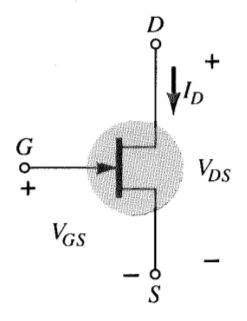
\includegraphics[height=5cm]{./Resources/fet_n.jpg}
		\caption{FET canal \textit{n}}
		\label{fet_symbol:1}
	\end{subfigure}
	\begin{subfigure}{.23\textwidth}
		\centering
		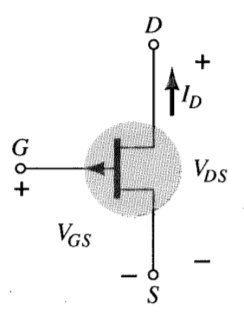
\includegraphics[height=5cm]{./Resources/fet_p.jpg}
		\caption{FET canal \textit{p}}
		\label{fet_symbol:2}
	\end{subfigure}
	\begin{subfigure}{.23\textwidth}
		\centering
		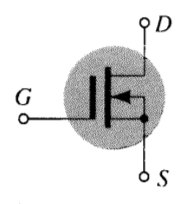
\includegraphics[height=3cm]{./Resources/mosfet_n.jpg}
		\caption{MOSFET canal \textit{n}}
		\label{fet_symbol:3}
	\end{subfigure}
	\begin{subfigure}{.23\textwidth}
		\centering
		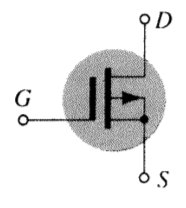
\includegraphics[height=3cm]{./Resources/mosfet_p.jpg}
		\caption{MOSFET canal \textit{p}}
		\label{fet_symbol:4}
	\end{subfigure}
	\captionsetup{justification=centering}
	\caption[S�mbolos do JFET e do MOSFET]{S�mbolos do JFET e do MOSFET. \\Fonte: BOYLESTAD (2011)}
	\label{fet_symbol}
\end{figure}

Os transistores do tipo FET/MOSFET s�o tamb�m conhecidos como resistores controlados por tens�o, o que ajuda a entender seu funcionamento: assumindo que h� uma DDP entre os terminais de \textit{dreno} e \textit{fonte} $V_{ds}$, a resist�ncia � passagem de corrente por estes terminais � controlada pela tens�o aplicada � \textit{porta} com rela��o � \textit{fonte} $V_{gs}$ do dispositivo. Quanto mais pr�ximo de zero � a tens�o, maior � o valor da resist�ncia, para os dispositivos FET e MOSFET intensifica��o \cite{boylestad}. Este comportamento � ilustrado na figura \ref{curva_fet} e a equa��o simplificada \ref{eq_fet_id} rege o comportamento de $I_{d}$ em fun��o de $V_{gs}$, na qual $I_{dss}$ e $V_{p}$ s�o os pontos not�veis no gr�fico da figura \ref{curva_fet} \cite{boylestad}.

\begin{figure}[H]
	\centering
	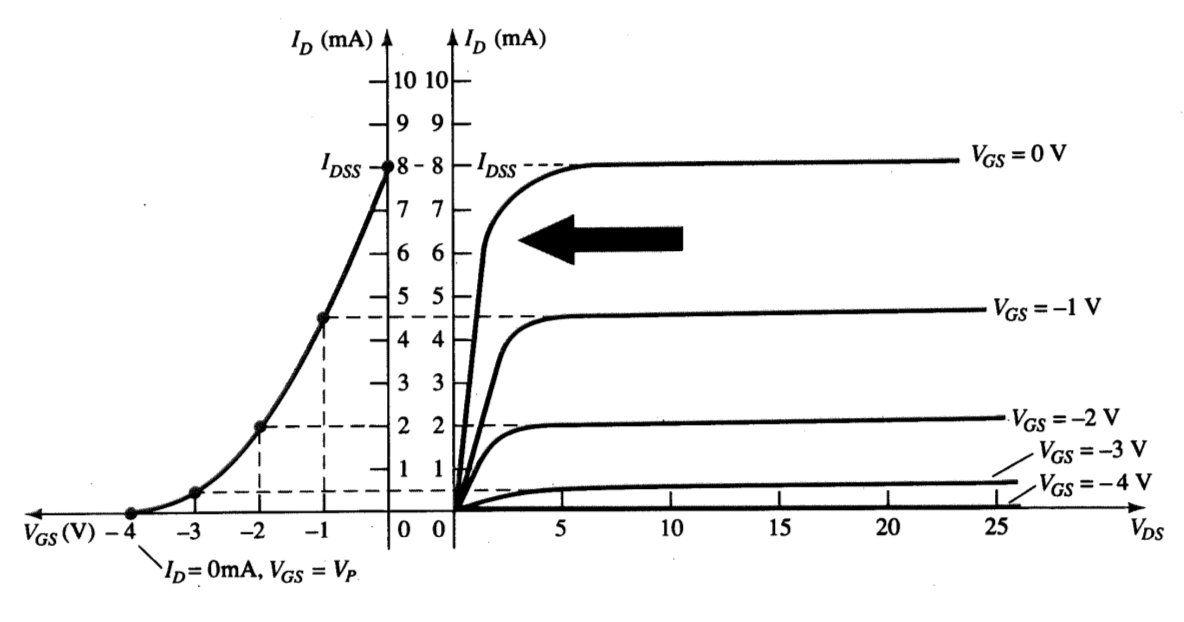
\includegraphics[scale=0.38]{./Resources/curva_fet.jpg}
	\captionsetup{justification=centering}
	\caption[Obtendo a curva de transfer�ncia das curvas de dreno de um JFET]{Obtendo a curva de transfer�ncia das curvas de dreno \\ Fonte: BOYLESTAD (2011)}
	\label{curva_fet}
\end{figure}

\begin{equation}
	\label{eq_fet_id}
	I_{d} = I_{dss} \left(1 - \frac{V_{gs}}{V_{p}}\right)^2
\end{equation}

De maneira an�loga ao BJT, tanto o FET quanto suas varia��es, aperfei�oamentos e aplica��es possuem uma teoria vasta, que n�o cabe a este trabalho detalhar. Para o aprofundamento no tema, recomenda-se a leitura da bilbiografia --- em especial de \cite{boylestad} e \cite{sedra}.

\subsection{Sensor de temperatura DS18B20}

O sensor de temperatura DS18B20, projetado pela Maxim, � um sensor digital que utiliza somente um pino de dados para comunica��o com o dispositivo \textit{master}, cujas regras s�o estabelecidas pelo protocolo propriet�rio de comunica��o \textit{1-Wire}\textregistered \cite{ds18b20}.

\textit{1-Wire} � um protocolo de comunica��o serial \textit{half-duplex} que utiliza uma linha para transmiss�o de dados, al�m da refer�ncia. � um protocolo de comunica��o \textit{master/slave}, ou seja, um dispositivo \textit{master} inicia a comunica��o e os dispositivos \textit{slave} somente respondem aos seus comandos. No caso deste protocolo espec�fico, todo dispositivo possui um identificador de 64 bits �nico, dentro do qual um byte indica o tipo do dispositivo. Devido ao seu modo de funcionamento, quando a linha de dados � desconectada, os dispositivos \textit{slave} entram em estado de \textit{reset}, o que favorece seu uso em aplica��es de contato. Enquanto a maioria destes dispositivos tem uma faixa de alimenta��o de 2,80-5,25V e n�o possui pino para alimenta��o \cite{onewire_ov} -- utilizando um sistema de alimenta��o parasita -- o sensor DS18B20 tem a possibilidade de alimenta��o parasita ou n�o e sua faixa tolerada para funcionamento � de 3-5,5V \cite{ds18b20}.

Uma vez que este protocolo de comunica��o foi concebido para opera��es nas quais os dispositivos \textit{master} e \textit{slave} est�o fisicamente muito pr�ximos, alguns cuidados devem ser observados ao utilizar linhas de transmiss�o de longas dist�ncias para manter a boa performance do sistema \cite{onewire_distance}. Como o estudo da Maxim acerca das implica��es do uso de linhas de longa dist�ncia negligencia este aspecto para redes com poucos dispositivos e cabeamento curto (menor que 10m), os cuidados de projeto das redes 1-wire n�o ser�o aqui especificados, deixando um aviso para trabalhos futuros que visem aplica��es de longas dist�ncias ou com n�mero elevado de dispositivos, a exemplo de uma microcervejaria de porte industrial.

Com rela��o a aspectos espec�ficos do sensor de temperatura, este apresenta precis�o de 0,5\si{\degree}C para a faixa de temperaturas de -10\si{\degree}C a +85\si{\degree}C, e de 2,0\si{\degree}C para a faixa completa de opera��o, de -55\si{\degree}C a +125\si{\degree}C. Quanto � resolu��o, esta pode ser programada de 9 a 12 bits, sendo 8 bits para a parte inteira e 1 a 4 bits decimais. O custo da melhor resolu��o � o aumento no tempo de convers�o de uma leitura para valor digital, variando de 93,75ms a 750ms para os casos extremos \cite{ds18b20}.

A arquitetura interna do CI � apresentada na figura \ref{18b_blocos}. Nota-se que o dispositivo, por utilizar o protocolo \textit{1-Wire}, tem uma ROM de 64 bits para identifica��o \cite{onewire_ov}, al�m de uma regi�o de mem�ria de rascunho, que consiste de uma mem�ria SRAM de 64 bits, dividida em 8 regi�es de 1 byte, para promover a interface com as funcionalidades do CI: sensor de temperatura, alarmes program�veis para estouro de valores m�nimo e m�ximo das medi��es, registrador de configura��o da resolu��o e gerador de c�digo CRC de 8 bits \cite{ds18b20}. A figura \ref{18b_mmap} apresenta o mapa de mem�ria do DS18B20 -- nota-se que os registradores de configura��o e alarme s�o copiados para uma mem�ria n�o vol�til (EEPROM) ap�s configurados pelo \textit{master}, retendo seus valores mesmo em caso de corte na alimenta��o. Outra informa��o �til obtida a partir da figura \ref{18b_mmap} � o valor da temperatura lido ap�s uma queda de alimenta��o, que � de +85\si{\degree} C at� que o dispositivo esteja pronto para uso \cite{ds18b20}.

\begin{figure}[H]
	\centering
	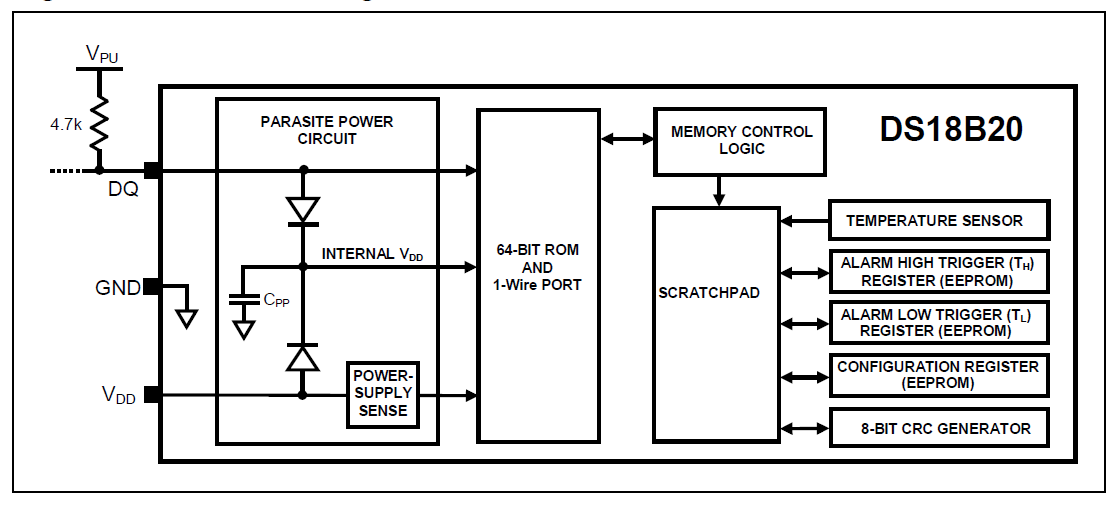
\includegraphics[width=12cm]{./Resources/ds18b20-blocos.png}
	\captionsetup{justification=centering}
	\caption[Arquitetura interna do DS18B20]{Arquitetura interna do DS18B20 \\Fonte: MAXIM INTEGRATED
	}
	\label{18b_blocos}
\end{figure}

\begin{figure}[H]
	\centering
	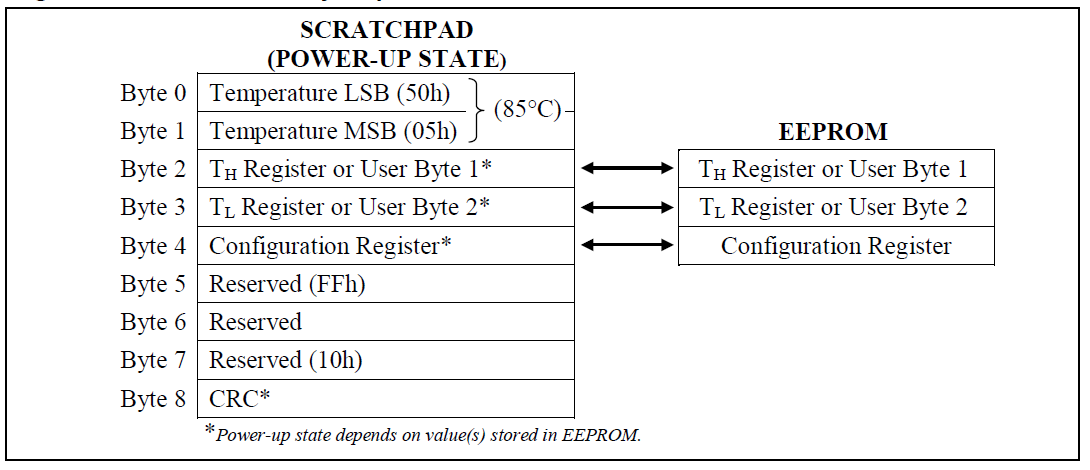
\includegraphics[width=11.83cm]{./Resources/ds18b20-mmap.png}
	\captionsetup{justification=centering}
	\caption[Mapa de mem�ria do DS18B20]{Mapa de mem�ria do DS18B20. \\Fonte: MAXIM INTEGRATED
	}
	\label{18b_mmap}
\end{figure}

As leituras de temperatura s�o feitas em dois bytes, LSB e MSB, representados na figura \ref{18b_formato}, e que juntos s�o uma representa��o em complemento de dois, sendo que os 5 bits mais significativos s�o redundantes e, para resolu��es menores do que 12 bits, o valor dos bits menos significativos � indefinido (1 bit indefinido para 11 bits de resolu��o; 2 bits indefinidos para 10 bits de resolu��o, etc).

\begin{figure}[H]
	\centering
	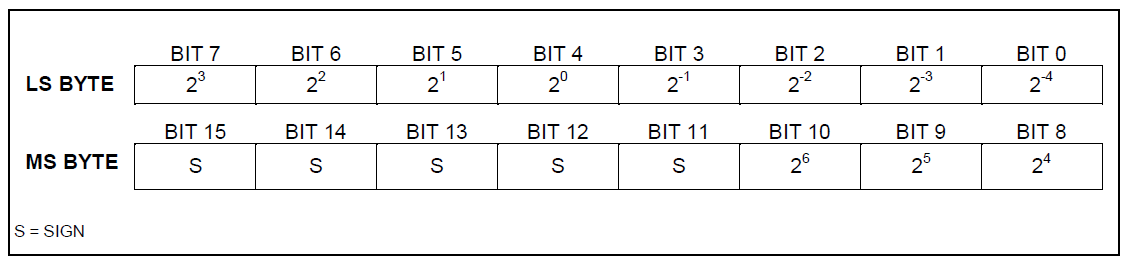
\includegraphics[width=11.83cm]{./Resources/ds18b20-formato.png}
	\captionsetup{justification=centering}
	\caption[Registradores de temperatura do DS18B20]{Registradores de temperatura do DS18B20. \\Fonte: MAXIM INTEGRATED
	}
	\label{18b_formato}
\end{figure}

O Kernel do Linux possui \textit{device drivers} que suportam parcialmente o uso do sensor DS18B20, portanto n�o h� a necessidade de descrever em detalhes o protocolo \textit{1-Wire}. O \textit{device driver} \textit{w1-gpio} controla o barramento (\textit{master}) \textit{1-wire} utilizando a API GPIO para controlar a linha, sendo que a porta utilizada � especificada utilizando dados espec�ficos da placa. O \textit{device driver} \textit{w1-therm} suporta algumas fam�lias de sensores de temperatura da Maxim (\textit{slave}), dentre elas a DS18*20, fazendo convers�es b�sicas de temperatura e fornecendo-as ao sistema por meio do FS (\textit{File System} ou Sistema de Arquivos). O resultado da abertura e leitura do arquivo correspondente a um sensor, � a convers�o de temperatura pelo \textit{driver} e posterior fornecimento dos dados recebidos pela placa, checagem do CRC e temperatura em \si{\degree}C/1000. Este driver n�o suporta convers�o de temperatura simult�nea de m�ltiplos sensores nem redu��o da precis�o de convers�o, portanto s� s�o poss�veis leituras de 12 bits. Em caso de alimenta��o parasita, somente um sensor pode estar conectado � linha por vez e, caso a placa ofere�a suporte a \textit{pull-up} interno, o driver � capaz de us�-lo \cite{onewire_kernel}.

%\subsection{Detector de passagem por zero}

%\subsection{\textit{Drivers} de pot�ncia}

%\subsection{Roteamento de placas de circuito impresso}

%\section{Servo-motor}

\section{Sistema de controle de temperatura}

\subsection{Controlador PID}

\subsection{Interface com sensores e atuadores}

\chapter{Materiais}

Este cap�tulo lista os materiais empregados no desenvolvimento deste projeto. 

\section{N�cleo do projeto}

Os materiais utilizados no n�cleo do mesmo est�o contidos na tabela \ref{bom_core}:

\begin{center}
	\begin{table}[H]
		\captionsetup{justification=centering}
		\caption[Lista de materiais que comp�em o n�cleo do projeto]{Lista de materiais que comp�em o n�cleo do projeto}
		\label{bom_core}
		\begin{tabular}{ | M{13cm} | M{2cm} |}
			\hline
			\textbf{Descri��o} & \textbf{Quantidade} \\ \hline
			BeagleBone Black Rev. C & 1\\ \hline
			Fonte de tens�o 5V/2A & 1\\ \hline
			Cart�o \si{\micro}SD 4GB & 1\\ \hline
			Adaptador Wi-Fi USB Ralink RT5370 & 1\\ \hline
			Sonda de a�o inoxid�vel � prova d'�gua com sensor DS18B20 & 1\\ \hline
		\end{tabular}
	\end{table}
\end{center}

\section{Sistema mec�nico}

Os materiais utilizados na constru��o da parte mec�nica do sistema est�o listados na tabela \ref{bom_mec}:

\begin{center}
	\begin{table}[H]
		\captionsetup{justification=centering}
		\caption[Lista de materiais utilizados na confec��o do subsistema mec�nico]{Lista de materiais utilizados na confec��o do subsistema mec�nico}
		\label{bom_mec}
		\begin{tabular}{ | M{13cm} | M{2cm} |}
			\hline
			\textbf{Descri��o} & \textbf{Quantidade} \\ \hline
			
			\textbf{Itens diversos} & \\ \hline
			Caldeir�o de alum�nio n.\si{\degree}36 (32 litros) & 2\\ \hline
			Resistor helicoidal com duas voltas, 110V/2200W & 2\\ \hline
			Fundo falso de a�o inoxid�vel circular \si{\phi}=36cm & 1\\ \hline
			Bomba centr�fuga magn�tica 12VDC Topsflo TL-B08H-12-1006 & 2\\ \hline
			Trocador de calor de contra-fluxo, tubo de alum�nio de 7m & 1\\ \hline
			Tecido mussalina x 1,5m (cent�metros) & 30\\ \hline
			
			\textbf{Tubula��o} & \\ \hline
			Mangueira silicone 3/8" (metros) & 1\\ \hline
			Mangueira cristal 3/8" (metros) & 2\\ \hline
			Mangueira cristal 1/2" (metros) & 7\\ \hline
			Tubo schedule S40 1/2" a�o inoxid�vel (metros) & 3\\ \hline
			
			\textbf{Valvulas e acessorios} & \\ \hline
			\textbf{V�lvulas e acess�rios} & \\ \hline
			V�lvula de reten��o portinhola 1/2" a�o inoxid�vel & 2\\ \hline
			V�lvula esfera lat�o, passagem plena 1/2" & 2\\ \hline
			V�lvula solen�ide 1/2" 12V pl�stico uso geral & 1\\ \hline
			V�lvula solen�ide Danfoss 1/2" EV210BD 032U3620 & 3\\ \hline
			Bobina Danfoss 15W 12VDC 042N7550 & 3\\ \hline
			
			\textbf{Conex�es e acess�rios} & \\ \hline
			Espig�o de lat�o com redu��o 1/2" - 3/8" & 3\\ \hline
			Bico de engate r�pido de pl�stico 1/2" & 1\\ \hline
			Engate r�pido de pl�stico 1/2" & 1\\ \hline
			Abra�adeira 3/8" & 4\\ \hline
			Abra�adeira 1/2" & 2\\ \hline
			Luva sextavada 1/2" lat�o & 1\\ \hline
			Arruela a�o inoxid�vel 1/2" & 4\\ \hline
			Anel de veda��o de silicone 1/2" & 4\\ \hline
			Contra porca a�o inoxid�vel 1/2" & 2\\ \hline
			Cotovelo f�mea 90\si{\degree} 1/2" a�o inoxid�vel & 1\\ \hline
			Cotovelo M/F 90\si{\degree} 1/2" a�o inoxid�vel & 1\\ \hline
			Tee f�mea 90\si{\degree} 1/2" a�o inoxid�vel & 4\\ \hline
			Niple duplo sextavado 1/2" a�o inoxid�vel & 9\\ \hline
			Espig�o sextavado 1/2" a�o inoxid�vel & 4\\ \hline 
		\end{tabular}
	\end{table}
\end{center}

\section{Componentes eletr�nicos}

Os componentes eletr�nicos utilizados para confec��o dos circuitos de interface com a BBB, acionamentos de pot�ncia e circuitos diversos est�o listados na tabela \ref{bom_eln}:

\begin{center}
	\begin{table}[H]
		\captionsetup{justification=centering}
		\caption[Lista de componentes eletr�nicos diversos empregados na confec��o de PCBs e cabeamento do sistema]{Lista de componentes eletr�nicos diversos empregados na confec��o de PCBs e cabeamento do sistema}
		\label{bom_eln}
		\begin{tabular}{ | M{6.5cm} | M{6.5cm} | M{2cm} |}
			\hline
			\textbf{Componente} & \textbf{Modelo/valor/descri��o} & \textbf{Quantidade} \\ \hline
			
			\textbf{Placa de acionamentos de pot�ncia} & & \\ \hline
			Capacitor cer�mico & 100nF & 1\\ \hline
			Capacitor poli�ster & 330nF & 1\\ \hline
			Resistor & 2,2k\si{\ohm} 1/4W 5\% & 10\\ \hline
			Resistor & 22k\si{\ohm} 1/4W 5\% & 10\\ \hline
			Optoacoplador & 4N25 DIP & 7\\ \hline
			Regulador de tens�o & LM7805 TO220 & 1\\ \hline
			Transistor MOSFET & IRF540N TO220 & 7\\ \hline
			Diodo retificador & 1N4007 & 6\\ \hline
			Conector para alimenta��o & J4 & 2\\ \hline
			Conector header & 10 vias & 1\\ \hline
			Borne KRE & 2 vias & 6\\ \hline
			Porta fus�vel & 25mm 6A(MAX) & 1\\ \hline
			Fus�vel de vidro & 20AG 5A 20mm & 1\\ \hline
			
			\textbf{Cabeamento} & & \\ \hline
			Conector latch & 10 vias & 1\\ \hline
			Cabo flat (metros) & 10 vias & 2\\ \hline
			
			\textbf{Componentes diversos} & & \\ \hline
			Fonte de tens�o & 12V/5A & 1\\ \hline
			Rel� de estado s�lido & Fotek SSR-25 DA (25A) & 2\\ \hline
			Cabo de cobre (metros) & 4mm se��o transversal & 6\\ \hline
			Tomada & 20A & 1\\ \hline
			Adaptador T & padr�o NEMA & 1\\ \hline
			Terminal anel & pr�-isolado M6 & 4\\ \hline
			Plug tomada & 20A padr�o NBR 14136 & 1\\ \hline
			Servo Motor & TowerPro MG995 & 1\\ \hline
			
		\end{tabular}
	\end{table}
\end{center}

\section{Equipamentos, instrumentos, \textit{softwares} e miscel�nea}

Os equipamentos, instrumentos de medi��o e demais objetos e/ou \textit{softwares} de suporte ao desenvolvimento do projeto est�o listados na tabela \ref{bom_sup}.

\begin{center}
	\begin{table}[H]
		\captionsetup{justification=centering}
		\caption[Lista de equipamentos, instrumentos e \textit{softwares} de suporte ao desenvolvimento do projeto]{Lista de equipamentos, instrumentos e \textit{softwares} de suporte ao desenvolvimento do projeto}
		\label{bom_sup}
		\begin{tabular}{ | M{10cm} | M{5cm} |}
			\hline
			\textbf{Descri��o} & \textbf{Detalhes} \\ \hline
			
			\textbf{Instrumentos de medi��o} & \\ \hline
			Oscilosc�pio Agilent DSO-X 2002A & 70MHz - 2 canais\\ \hline
			Mult�metro Minipa ET-2110 & \\ \hline
			
			\textbf{\textit{Softwares}} & \\ \hline
			MATLAB & vers�o\\ \hline
			FreeCAD & v. 0.15\\ \hline
			MatterControl & v. 1.3.0 + plugin CNCBrasil\\ \hline
			Cura & v. 15.06.03\\ \hline
			Putty & \\ \hline
			
			
			\textbf{Diversos} & \\ \hline
			Impressora 3D & CNCBrasil Standard\\ \hline
			Filamento para impress�o 3D & ABS 1,75mm\\ \hline

			\textbf{Controle de vers�o} & \\ \hline
			GitHub & \url{https://github.com/leograba/final_paper_tcc}\\ \hline
			Filamento para impress�o 3D & ABS 1,75mm\\ \hline
			
		\end{tabular}
	\end{table}
\end{center}

\section{Insumos cervejeiros}

A descri��o dos insumos cervejeiros utilizados para confec��o da receita e posterior teste do sistema pode ser encontrada na tabela \ref{bom_recipe}.

\begin{center}
	\begin{table}[H]
		\captionsetup{justification=centering}
		\caption[Lista insumos cervejeiros para produ��o de cerveja do tipo \textit{Blond Ale}]{Lista insumos cervejeiros para produ��o de cerveja do tipo \textit{Blond Ale}}
		\label{bom_recipe}
		\begin{tabular}{ | M{13cm} | M{2cm} |}
			\hline
			\textbf{Descri��o} & \textbf{Quantidade} \\ \hline
			Malte Pilsen (kg) & 4,5\\ \hline
			Malte Munich (kg) & 0,5\\ \hline
			L�pulo Hallertauer Tradition (g) & 50\\ \hline
			Levedura desidratada Safale S-04 (Tipo Ale inglesa) sach� & 1\\ \hline
			Sanitizante Iodophor dilu�do em �gua (ml/l) & 0,8\\ \hline
		\end{tabular}
	\end{table}
\end{center}

% % % % % % % % % % % % % % % % % % % % % % % % % % % % % % % % % % % % % % % % % % % % % % % % % % %
\chapter{M�todos}

Este cap�tulo descreve todos os procedimentos de projeto e testes, dentre outros,  empregados visando a obten��o do resultado final deste trabalho. Os procedimentos aqui empregados s�o embasados na teoria apresentada no cap�tulo \ref{EmbasamentoTeorico}. Cabe salientar que, embora este seja um projeto de integra��o entre \textit{mec�nica}, \textit{hardware} e \textit{software}, os esfor�os foram concentrados na �rea de desenvolvimento de \textit{softwares}, desde o \textit{firmware} da PRU-ICSS integrado ao servidor Apache posteriormente migrado para Node.js, at� a aplica��o de usu�rio, escrita em diversas linguagens, de programa��o ou n�o --- a exemplo de HTML e CSS.

%%%%%%%%%%%%%%%%%%%%%%%%%%%%%%%%%%%%%%%%%%%%%%%%%%%%%%%%%%%%%%%%%%%

\section{Estrutura mec�nica}
\label{estmec}

Para o projeto da parte mec�nica, em primeiro lugar foi concebida uma configura��o de sistema baseada tanto na literatura dispon�vel quanto em projetos de sistemas dispon�veis para aquisi��o no mercado: um sistema de duas panelas an�logas � MT e ao BK, sendo que durante o processo de cozimento do mosto, o BK pudesse ser utilizado como HLT e, portanto, fez-se necess�rio o projeto de um sistema de recircula��o entre as duas panelas. Obserava-se que esta proposta representa um h�brido entre um sistema de 3 panelas tradicional - que consiste de uma panela para mostura��o, uma para lavagem dos gr�os, ou sparging, e uma para fervura; e o sistema popularizado pela Braumeister, composto de 1 panela, com recircula��o. Esta abordagem permite a economia financeira e simplifica��o mec�nica do sistema de tr�s panelas com o benef�cio do \textit{sparging} inexistente no sistema de uma panela.

\subsection{Funcionamento da estrutura}

Na figura \ref{esboco} � apresentada uma representa��o esquem�tica da parte funcional.

\begin{figure}[H]
	\centering
	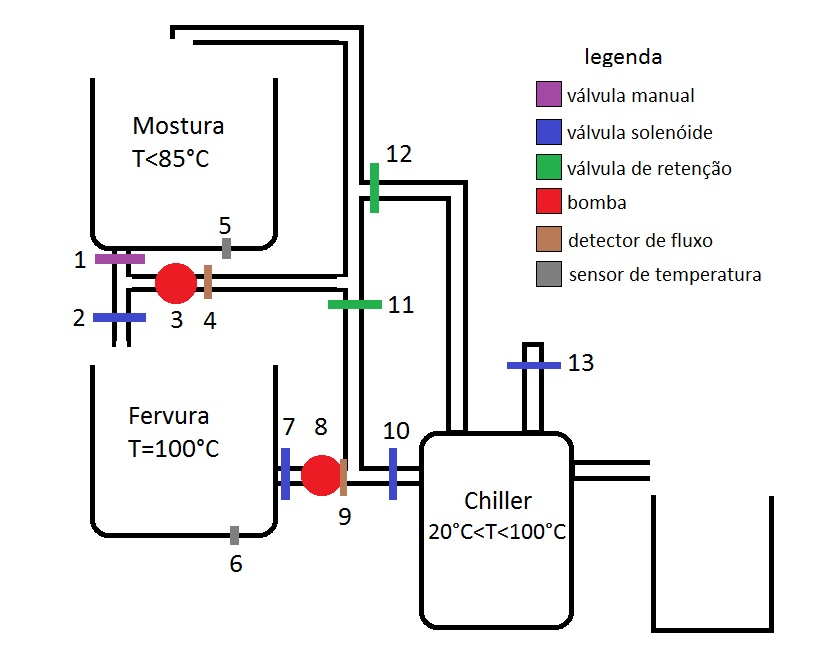
\includegraphics[scale=0.55]{./Resources/esb_mec.jpg}
	\captionsetup{justification=centering}
	\caption[Representa��o esquem�tica da estrutura mec�nica]{Representa��o esquem�tica da estrutura mec�nica}
	\label{esboco}
\end{figure}

Na panela superior ou MT, rotulada como \textit{Mostura}, os gr�os s�o adicionados ap�s o aquecimento inicial da �gua:

\begin{itemize}
	\item A v�lvula 1 � uma v�lvula manual do tipo esfera, com passagem plena. Durante a opera��o do equipamento ela deve ficar sempre aberta, portanto seu uso � realizado somente em caso de emerg�ncias.
	\item Ap�s a adi��o dos gr�os, a bomba 3 � ligada para que o l�quido da panela seja recirculado. As v�lvulas de reten��o 11 e 12 n�o permitem que o l�quido passe por elas, portanto sobra somente um caminho poss�vel para este, que � ascender na tubula��o at� entrar novamente na MT. Note-se que n�o h� v�lvula automatizada na sa�da da MT, uma vez que o mosto fica em recircula��o constante ao longo do processo de cozimento.
	\item Ap�s a mostura a bomba 3 � desligada e a v�lvula solen�ide 2 � aberta, escoando o l�quido para a panela de fervura BK. Simult�neamente, a v�lvula solen�ide 7 e a bomba 8 s�o ativadas, fazendo com que a �gua de lavagem presente na BK/HLT flua pela tubula��o at� a MT, iniciando o processo de \textit{sparging}. Durante um tempo predefinido, o mosto e a �gua de lavagem recirculam pelas duas panelas e se misturam.
	\item Durante a fervura, as v�lvulas 2 e 7 s�o fechadas. Neste per�odo a MT deve ser esvaziada, j� que ela ser� usada posteriormente para armazenamento da �gua de esfriamento do mosto --- �gua usada para limpeza do sistema e que reduz a produ��o de efluentes do mesmo.
	\item Ap�s a fervura, as v�lvulas solen�ides 7 e 10 s�o ativadas, permitindo o escoamento do l�quido para o trocador de calor. Simult�neamente a v�lvula solen�ide 13 � aberta e �gua fria circula em contra-fluxo para resfriar o mosto. Esta �gua sai quente do trocador de calor e passa pela v�lvula de reten��o 12, preenchendo a parte superior da tubula��o e sendo armazenada na MT para posterior limpeza do sistema.
	\item O mosto que sai resfriado do \textit{chiller} cai no balde de fermenta��o. Neste processo o l�quido entra em contato com o ar, o que � n�o somente desej�vel como essencial para o sucesso da fermenta��o, portanto esta � a �ltima parte do processo automatizada. Uma solu��o futura e que permite automa��o � o uso de um aerador em conjunto com um tanque de fermenta��o selado.
\end{itemize}

Para o bom funcionamento do sistema proposto, algumas condi��es devem ser atendidas:

\begin{itemize}
	\item Se o volume total de l�quido nas duas panelas ao final da mostura exceder o volume da BK, ela transbordar�. Por este motivo � importante que exista um sistema de detec��o de transbordo. Ainda assim, deve-se requisitar que o usu�rio do sistema calcule corretamente as propor��es da receita, pois apesar do sistema autom�tico anti-transbordo, ocorrer� perda de insumos devido ao ac�mulo de mosto inutiliz�vel na MT em caso de erro.
	\item S�o necess�rios filtros de material particulado para o bom funcionamento das v�lvulas e bombas \cite{danfoss_solenoid}.
	\item Os dispositivos mec�nicos (v�lvulas, bombas, tubula��o, dentre outros) e eletr�nicos (sensores e atuadores) em contato com o sistema mec�nico devem ser apropriados �s altas temperaturas impostas pela natureza do processo \cite{danfoss_solenoid, jefferson_solenoid}.
	\item As panelas, tendo como refer�ncia seu fundo, n�o devem ser alinhadas conc�ntricas, j� que isto torna a adi��o de l�pulos e o processo de manuten��o do equipamento desajeitados.
	\item A automa��o da t�cnica de \textit{whirlpool} n�o � contemplada nesta configura��o de sistema. Se o usu�rio a considera necess�ria, ele deve se encarregar de execut�-la manualmente.
	\item A �nica v�lvula com press�o suficiente para ser servo-operada � a 13, assumindo-se que a press�o incidente sobre ela seja maior do que 0,5bar, portanto as outras devem ser de opera��o direta \cite{danfoss_solenoid, jefferson_solenoid}.
	\item A limpeza automatizada, ou CIP, n�o � contemplada nesta configura��o do sistema, devido � alta complexidade \cite{cip_pres}, conforme indica a figura \ref{cip_system}, e ao custo de implementa��o proibitivo para este trabalho. N�o obstante, � recomendado ao usu�rio do sistema que fa�a a limpeza do mesmo t�o r�pido quanto poss�vel ap�s o final da produ��o.
\end{itemize}

\begin{figure}[H]
	\centering
	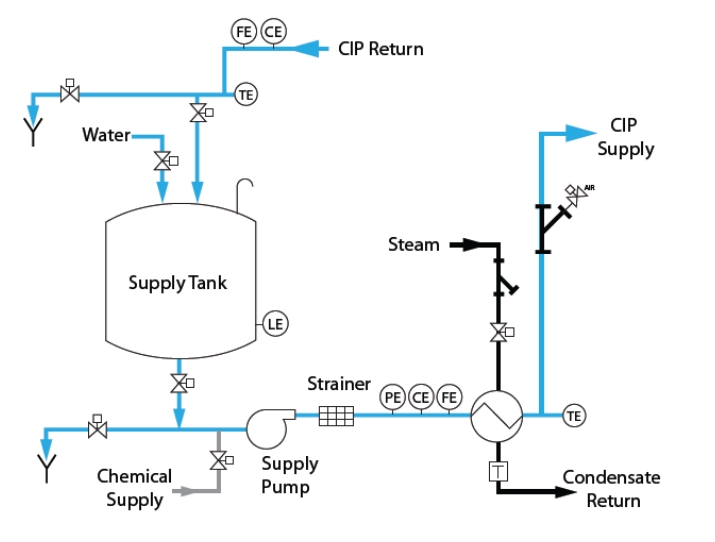
\includegraphics[scale=0.55]{./Resources/cip_example.jpg}
	\captionsetup{justification=centering}
	\caption[Sistema CIP b�sico]{Sistema CIP b�sico. \\Fonte: ROSE e MONTGOMERY (2010)}
	\label{cip_system}
\end{figure}

\subsection{Dimensionamento da parte funcional} 

Com a filosofia de opera��o do sistema mec�nico definida, � poss�vel realizar o dimensionamento deste sistema. A primeira considera��o a ser feita � que os materiais e m�todos aqui empregados n�o seguem nenhuma norma que permita o uso deste equipamento para fabrica��o de cerveja para venda --- tal escolha � feita em fun��o do alto custo de um sistema completamente dentro das normas e tamb�m pelo fato de este ser um trabalho cujo foco � a automa��o e o acesso remoto.

N�o obstante, o material da tubula��o escolhido foi o a�o inoxid�vel AISI304. J� que o volume de l�quido a ser trabalhado � pequeno, menor do que 40 litros, e a press�o de trabalho n�o � maior do que a press�o das bombas escolhidas posteriormente, foi decidido o uso de tubula��o de di�metro de 1/2" (21,34mm de di�metro externo) e espessura da parede no padr�o Schedule 40 (2,77mm de espessura). Embora esta espessura seja superdimensionada para a presente aplica��o, o mec�nico respons�vel pela montagem do sistema a requisitou para que fosse poss�vel fazer rosca sem danificar a integridade dos tubos. As conex�es, seguindo a escolha dos tubos, tamb�m s�o de a�o inoxid�vel de 1/2".

As liga��es entre tubos, conex�es e outros componentes do sistema s�o liga��es rosqueadas. Este � um meio de liga��o antigo, por�m de baixo custo, f�cil execu��o e usualmente empregadas em tubula��es de di�metro nominal pequeno, menor do que 4" \cite{ifba}. Para veda��o foi escolhido o Teflon, uma vez que � um material de baixo custo e alta disponibilidade e o padr�o de rosca adotado neste projeto � o BSP, baseado na norma ISO. Cabe salientar que, embora as liga��es rosqueadas sejam permitidas sob certas circunst�ncias na pr�tica, elas s�o relegadas a instala��es de baixa responsabilidade \cite{ifba}.

As panelas foram escolhidas no material de alum�nio, em fun��o do custo proibitivo do a�o inoxid�vel. S�o caldeir�es padr�o utilizados no ramo de hotelaria e restaurantes e dispon�veis em v�rios volumes. As duas panelas utilizadas neste trabalho tem capacidade para 32 litros e di�metro do fundo de 36cm, portanto sua especifica��o no mercado � \textit{caldeir�o de alum�nio n. 36}. Tal volume, 60\% superior ao da produ��o m�xima aconselhada, � necess�rio devido ao volume dos gr�os, � quantidade da �gua de lavagem e �s perdas por evapora��o que exigem uso de um volume de �gua inicial superior ao nominal.

O par�metro inicial escolhido para sele��o das v�lvulas solen�ide foi a temperatura m�xima de opera��o, cuja fonte de dados de opera��o � fornecida pelos fabricantes. Em seguida, foi escolhida uma veda��o adequada: os dois tipos mais comums de veda��o com suporte a temperatura de pelo menos 100\si{\degree}C s�o o EPDM e FKM (etileno-propileno-dieno e fluoreto de vinilideno, respectivamente) \cite{danfoss_solenoid}. Estes materiais possuem uma tabela de compatibilidade de fluidos cuja classifica��o pode ser satisfat�ria, boa, duvidosa, insatisfat�ria e desconhecida --- tanto para cerveja quanto para o mosto, ambas as veda��es s�o classificadas como satisfat�rias, embora para �gua a classifica��o do FKM seja somente boa \cite{epdm_fkm}. Por fim, um par�metro que foi verificado antes da escolha final das v�lvulas � a posi��o de opera��o, que varia conforme os modelos do fabricante \cite{danfoss_solenoid}. Com base nos par�metros supracitados, foi decidido usar:

\begin{itemize}
	\item V�lvula solen�ide 1/2" 12V pl�stico uso geral para �gua de resfriamento do trocador de calor.
	\item V�lvula solen�ide Danfoss 1/2" EV210BD 032U3620 para demais v�lvulas.
	\item Bobina Danfoss 15W 12VDC 042N7550 para acionamento das solen�ides Danfoss.
\end{itemize}

Informa��es t�cnicas sobre a v�lvula EV210BD 032U3620 est�o no anexo \ref{Anexo3} e sobre a bobina 042N7550 no anexo \ref{Anexo4}.

As bombas de recircula��o foram escolhidas com base na temperatura de opera��o e grau aliment�cio. Posteriormente, tanto a vaz�o quanto a perda de carga do sistema foram estimadas para verificar se a bomba escolhida seria adequada: o modelo Topsflo B08H-12-1006 tem capacidade m�xima de vaz�o de 10l/min e carga expressa em coluna de �gua de 6m. Como a capacidade m�xima do sistema � de 20l e idealmente a temperatura deve subir � taxa de 1\si{\degree}C/min, al�m de que a altura do sistema � menor do que 2m e as perdas de carga foram consideradas desprez�veis para este caso, foi decidido que a bomba escolhida � adequada ao projeto. No \ref{Anexo5} encontra-se a folha de dados t�cnicos do dispositivo.

Quanto �s conex�es, a figura \ref{conexoes_rascunho} apresenta um diagrama conceitual do sistema, contendo todas as pe�as necess�rias para a montagem do mesmo:

\begin{figure}[H]
	\centering
	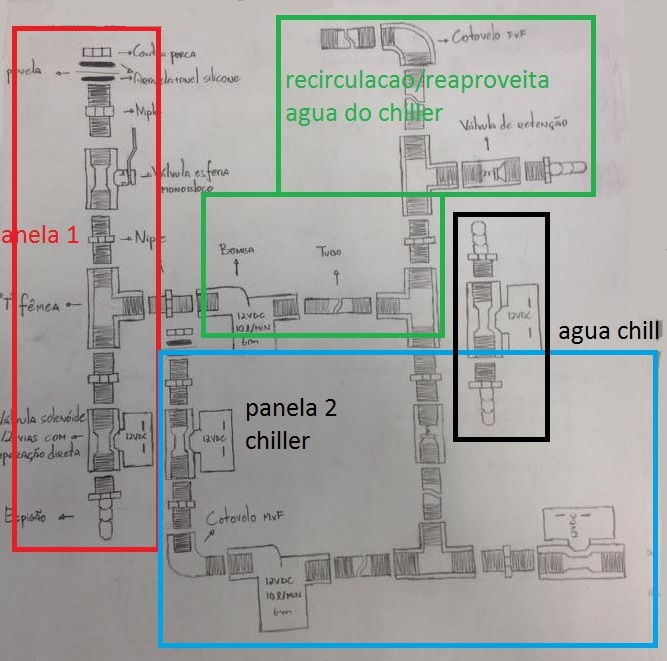
\includegraphics[scale=0.55]{./Resources/conexoes.jpg}
	\captionsetup{justification=centering}
	\caption[Diagrama conceitual das conex�es mec�nicas]{Diagrama conceitual das conex�es mec�nicas}
	\label{conexoes_rascunho}
\end{figure}

Na figura \ref{mt_cad} � apresentado um diagrama da MT constru�do no software FreeCAD, � qual est�o conectados o resistor de pot�ncia e um niple com veda��o. Tamb�m est�o presentes na figura a v�lvula esfera manual, um \textit{tee} f�mea, uma v�lvula Danfoss EV210B e tr�s niples de conex�o entre estes componentes. O modelo da v�lvula foi obtido a partir do website da Danfoss e importado, enquanto a modelagem dos outros componentes foi desenvolvida na plataforma FreeCAD. Na figura \ref{mt_cad_close} s�o apresentadas em detalhe as conex�es do resistor e do niple � panela e, por isto, a estrutura da mesma foi omitida. Os itens em amarelo s�o contra-porcas, em azul arruelas e, em vermelho an�is de veda��o (\textit{o-rings}).

\begin{figure}[H]
	\centering
	\begin{subfigure}{.46\textwidth}
		\centering
		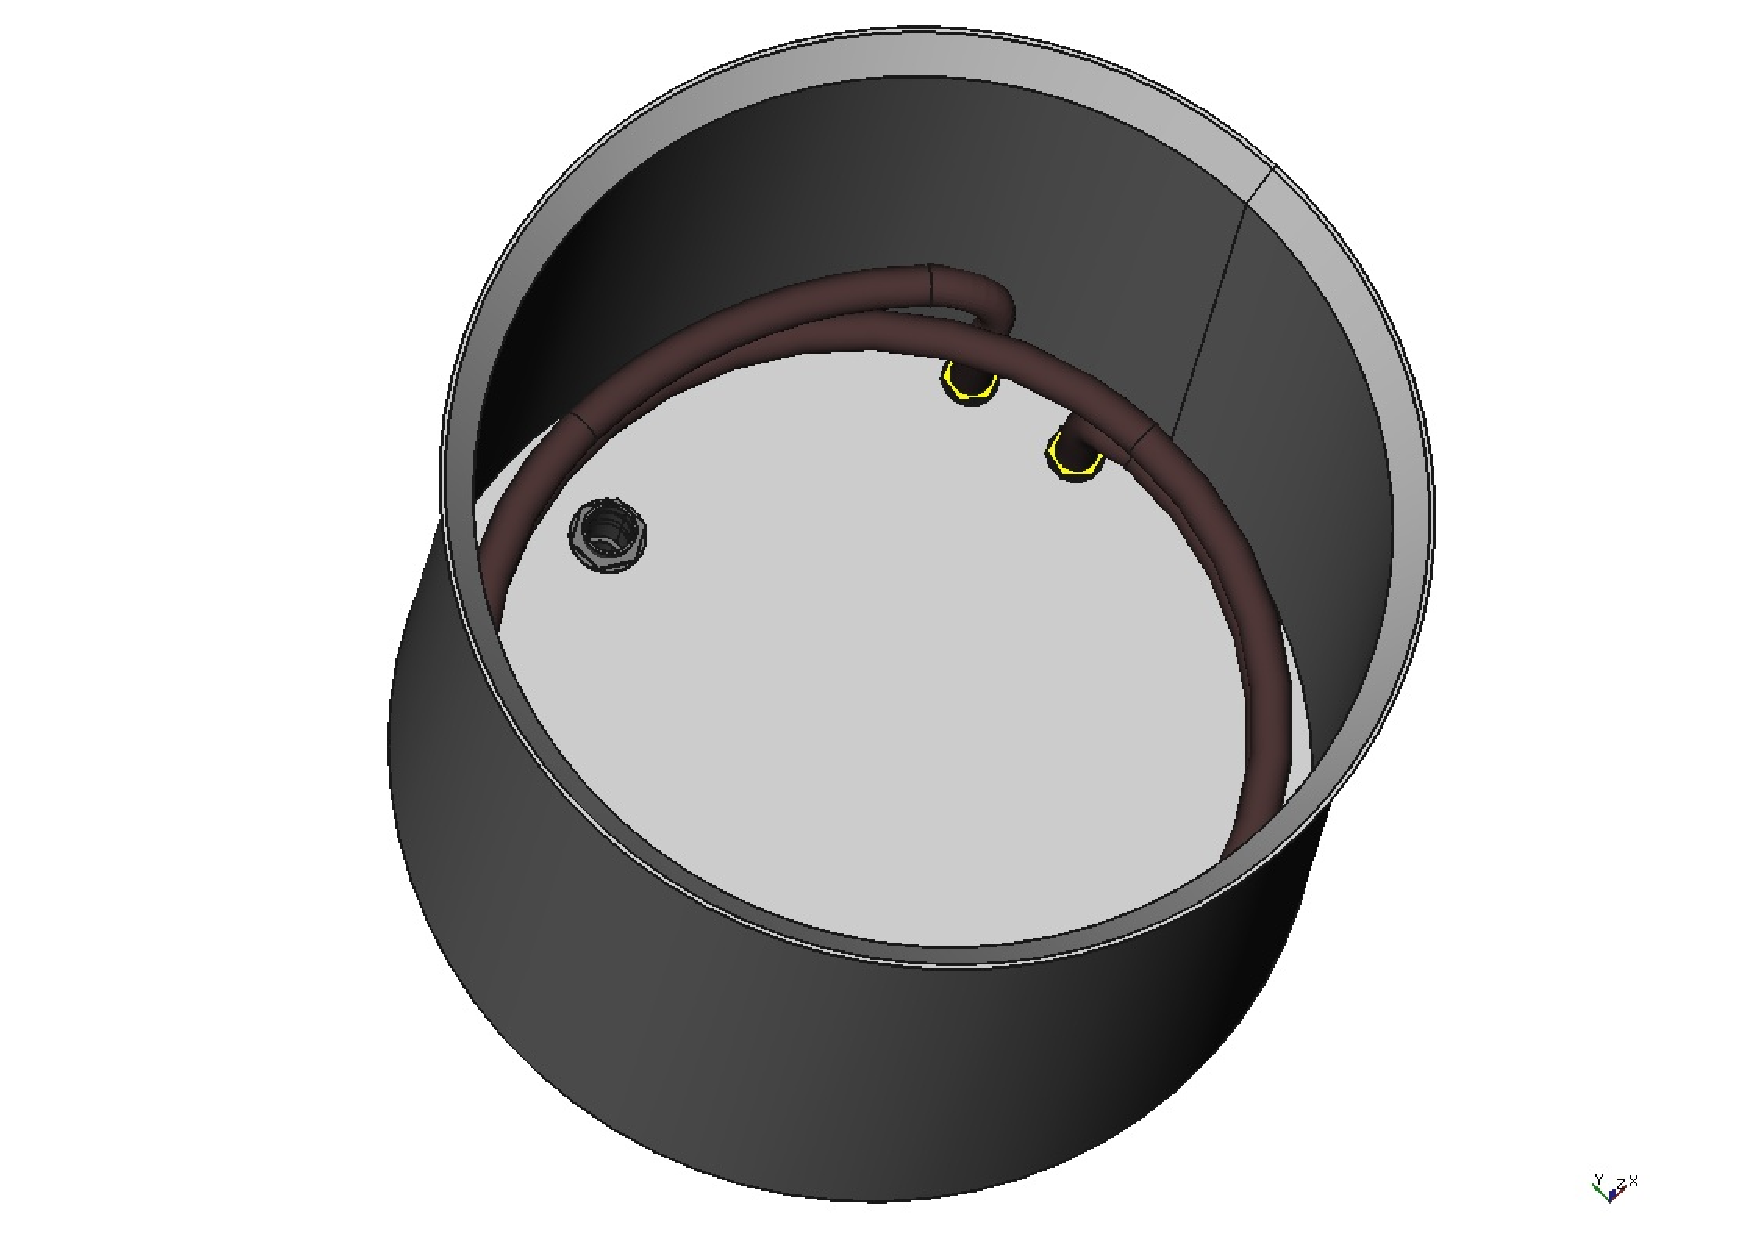
\includegraphics[height=5cm]{./Resources/mecsys/mash-tun-top-color.pdf}
		\caption{Vista superior}
		\label{mt_cad:1}
	\end{subfigure}
	\begin{subfigure}{.46\textwidth}
		\centering
		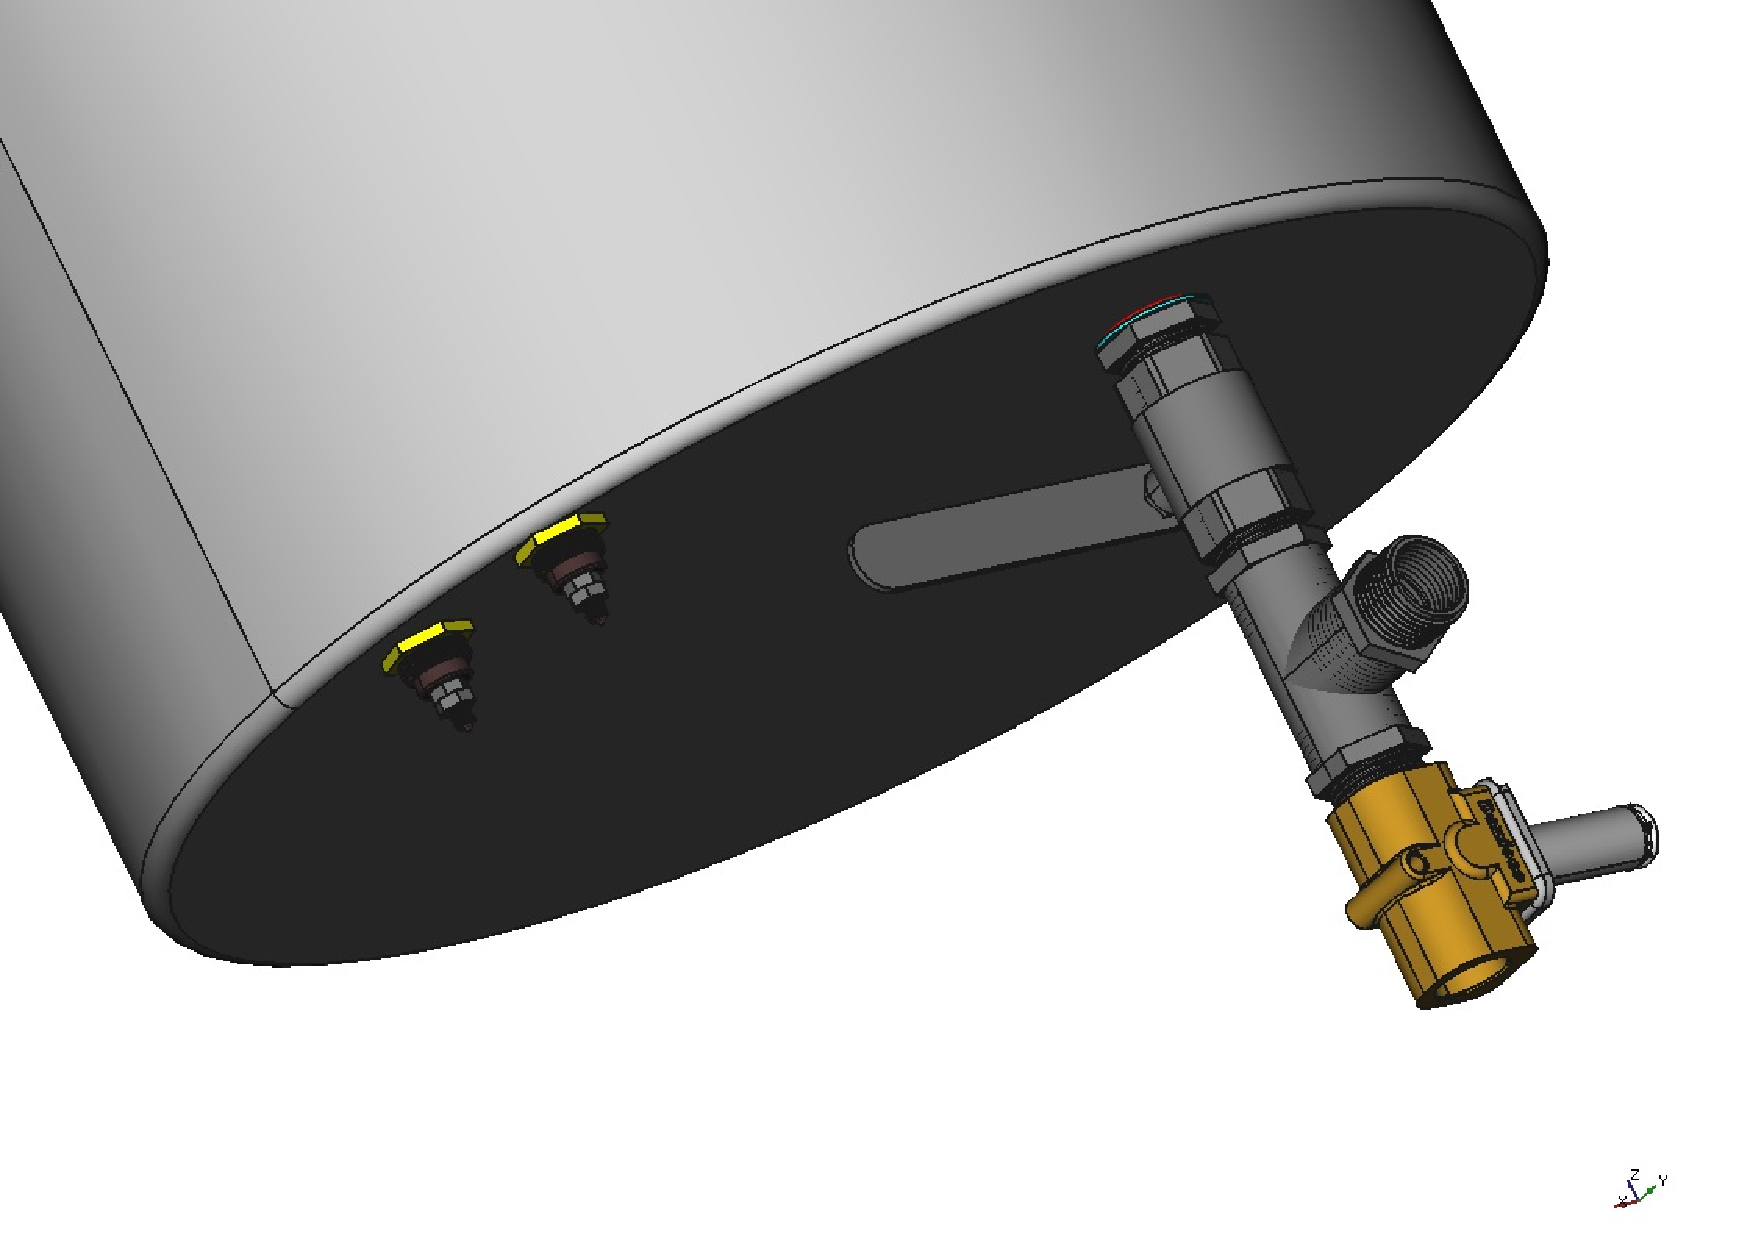
\includegraphics[height=5cm]{./Resources/mecsys/mash-tun-bottom-color.pdf}
		\caption{Vista inferior}
		\label{mt_cad:2}
	\end{subfigure}
	\captionsetup{justification=centering}
	\caption[Diagrama da panela de mostura e conex�es]{Diagrama da panela de mostura e conex�es}
	\label{mt_cad}
\end{figure}

\begin{figure}[H]
	\centering
	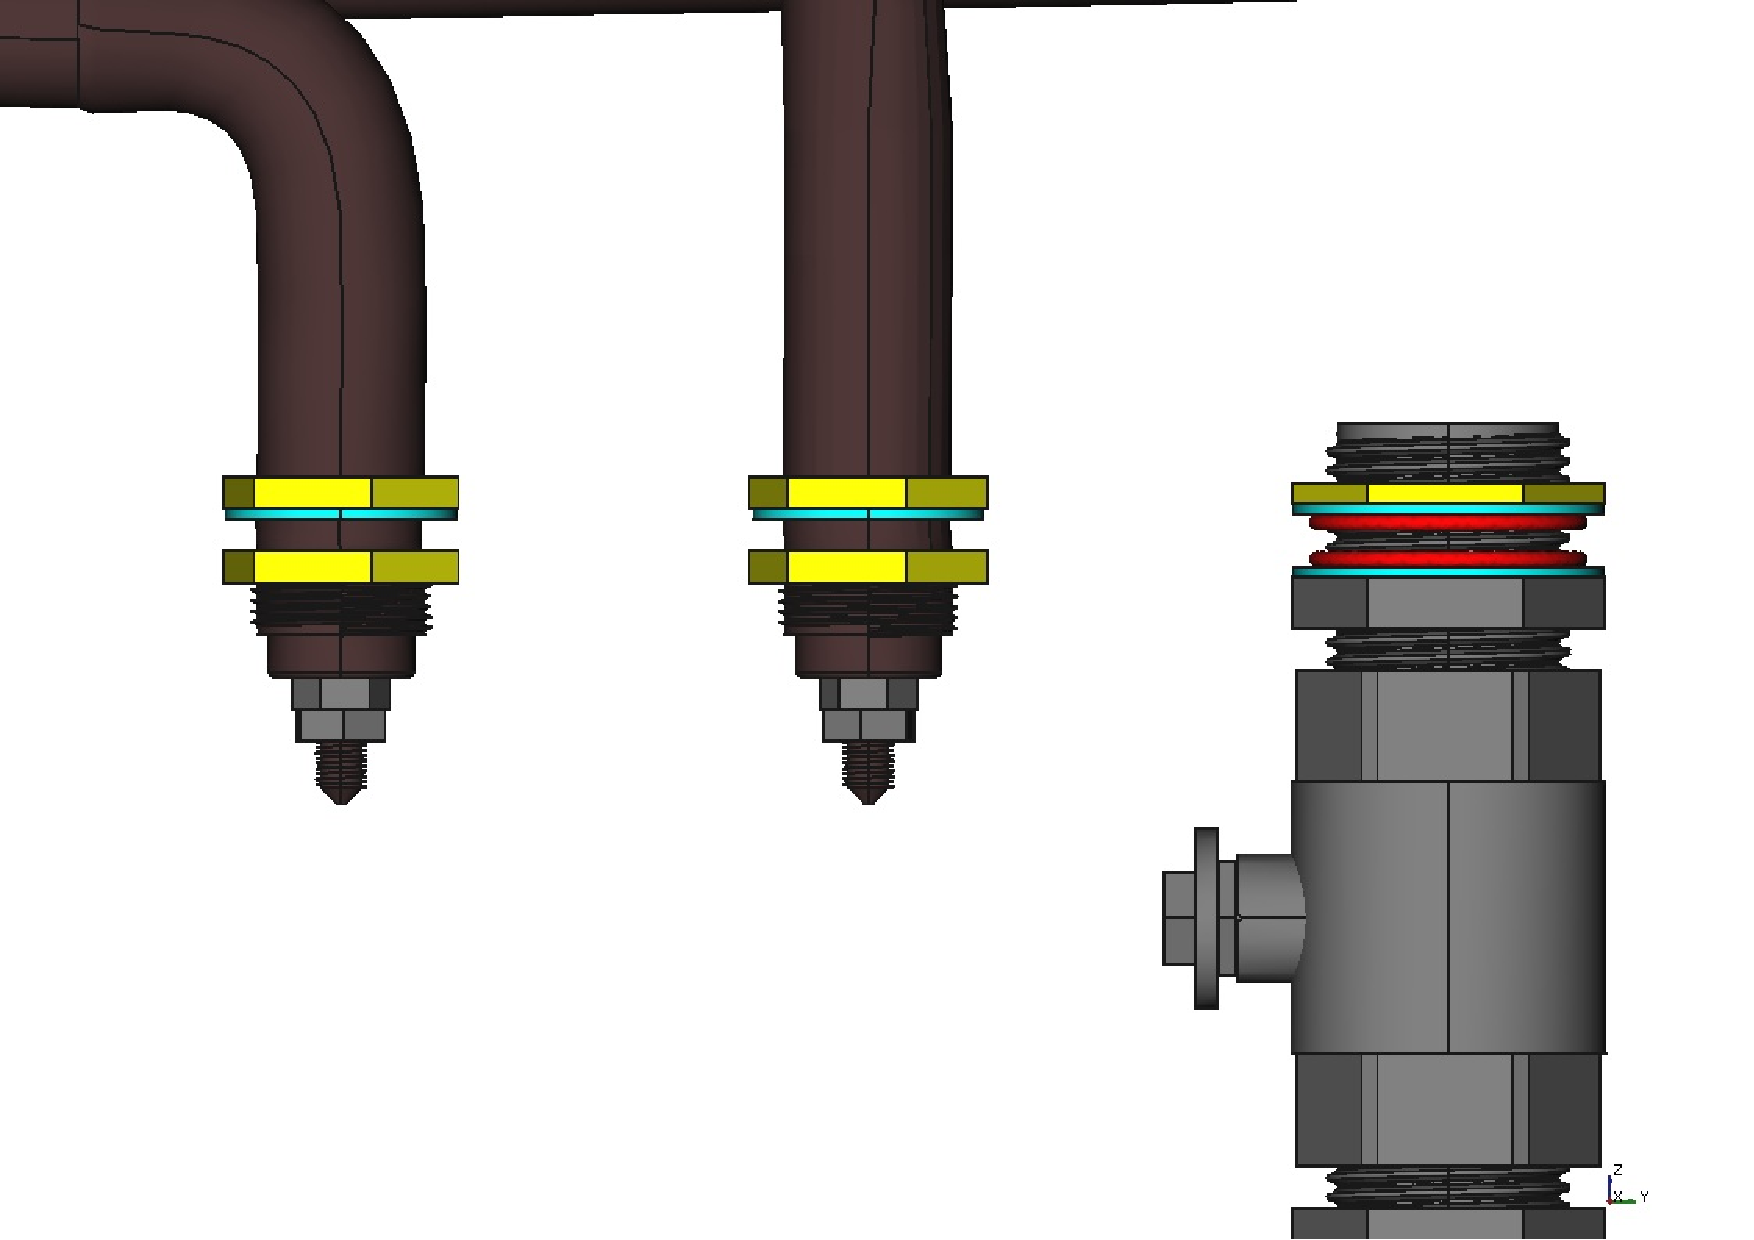
\includegraphics[scale=0.35]{./Resources/mecsys/mash-tun-seal-color.pdf}
	\captionsetup{justification=centering}
	\caption[Detalhes da veda��o da panela de mostura]{Detalhes da veda��o da panela de mostura}
	\label{mt_cad_close}
\end{figure}

\subsection{Estrutura met�lica de suporte}

Parte importante do projeto � o dimensionamento da estrutura met�lica de suporte �s panelas, j� que esta � respons�vel n�o somente pelo alojamento do sistema mec�nico como tamb�m pela facilidade de manuten��o. Para defini��o da altura das panelas, foram observadas primeiramente as alturas das panelas, da estrutura de adi��o de l�pulos (que ser� detalhada � parte na se��o \ref{hopbox}) e do \textit{chiller}. Na sequ�ncia, foi estimado um espa�o de manobra entre as duas panelas e uma altura m�nima do ch�o, com base na figura \ref{esboco}. Todas as medidas citadas est�o dispostas na tabela \ref{alturas}.

\begin{center}
	\begin{table}[H]
		\captionsetup{justification=centering}
		\caption[Dimens�es elementos mec�nicos relevantes para o projeto da altura da estrutura met�lica]{Dimens�es elementos mec�nicos relevantes para o projeto da altura da estrutura met�lica}
		\label{alturas}
		\begin{tabular}{ | M{10cm} | M{5cm} |}
			\hline
			\textbf{Descri��o} & \textbf{Altura (cm)} \\ \hline
			Panela BK & 30,0\\ \hline
			Panela MT & 30,0\\ \hline
			\textit{Chiller} & 30,0\\ \hline			
			Estrutura dos l�pulos aberta & 20,0\\ \hline
			V�o livre entre panelas & 20,0\\ \hline
			V�o do \textit{chiller} ao BK & 10,0\\ \hline
			Espa�o entre MT e topo & 10,0\\ \hline
		\end{tabular}
	\end{table}
\end{center}

Somando as alturas medidas e estimadas, obteve-se que a estrutura met�lica deve ter 1,5m de altura. A largura deve ser de 36,5cm para acomodar as panelas somente com uma pequena folga e o comprimento escolhido � de 70cm, o que permite alinhar as panelas de maneira n�o conc�ntrica, conforme abordado na se��o \ref{estmec} --- este valor � suficiente, j� que o di�metro somado das duas panelas � de 72cm e deve haver ao menos uma intersec��o para permitir o escoamento por gravidade da MT ao BK. Na figura \ref{estmec_cad} � apresentado o projeto da estrutura j� com as prateleiras para acomodar as panelas. Note-se que foram escolhidas cantoneiras de 2" x 1/8" para a constru��o deste equipamento.

\begin{figure}[H]
	\centering
	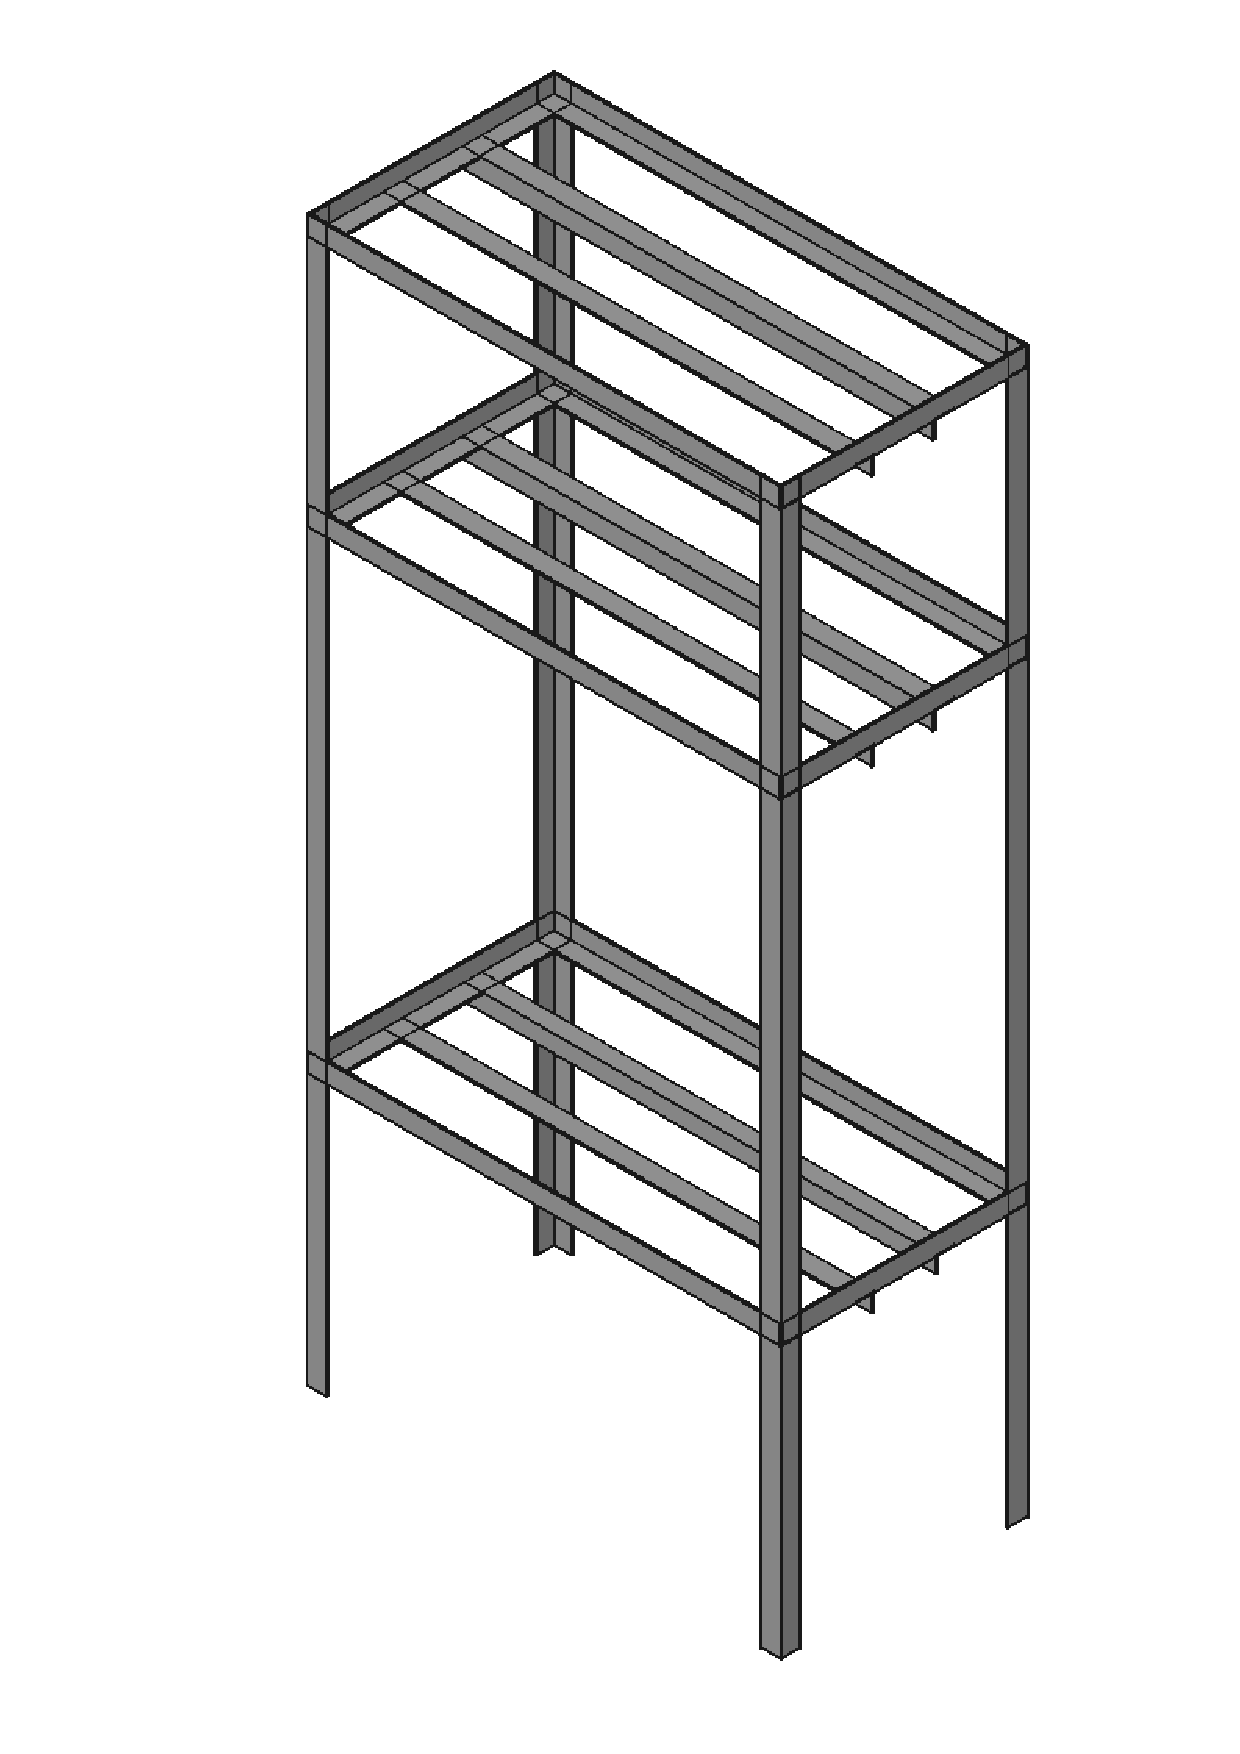
\includegraphics[scale=0.35]{./Resources/mecsys/estmec-freecad.pdf}
	\captionsetup{justification=centering}
	\caption[Projeto da estrutura met�lica]{Projeto da estrutura met�lica}
	\label{estmec_cad}
\end{figure}

%%%%%%%%%%%%%%%%%%%%%%%%%%%%%%%%%%%%%%%%%%%%%%%%%%%%%%%%%%%%%%%%%%%%%%%%%%

\section{Estrutura de adi��o de l�pulos}
\label{hopbox}

Devido � necessidade de adicionar l�pulos � receita em propor��es e tempos predefinidos, foi necess�rio o projeto de uma estrutura autom�tica de adi��o de l�pulos. Em fun��o das in�meras possibilidades de combina��es de l�pulos e temporiza��es, a escolha natural do projeto foi uma estrutura que permita esta flexibilidade --- uma caixa com oito compartimentos separados para adi��o sequencial destes insumos. Com base em um pacote de l�pulos em \textit{pellets} de 50g, estimou-se que seu volume � de $160cm^3$ e, sabendo-se que uma receita de 20l dificilmente utiliza uma quantidade maior do que 400g de l�pulos, a decis�o tomada foi a de que cada um dos 8 compartimentos deveria ter os $160cm^3$ necess�rios para acomodar 50g. Para confirmar que 400g � uma quantidade razo�vel, foi seguido o c�lculo de IBU de \cite{palmer}, detalhado no ap�ndice \ref{Ap�ndice C}.

Fixando a altura do compartimento em 10,0cm foram escolhidos valores de comprimento e largura de 16,0cm e 8,0cm respectivamente, assumindo inicialmente que as paredes das divis�rias tem espessura desprez�vel. A equa��o para volume de um prisma e a escolha das dimens�es s�o demonstradas em \ref{eq_hop_vini}:

\begin{subequations}
	\label{eq_hop_vini}
	\begin{align}
		V &= l\cdot w\cdot h = V_{50g}\cdot 8 \\
		&= l\cdot w\cdot 10 = 160\cdot 8 \nonumber \\
		l\cdot w\cdot &= 128, fixando \quad l = 16cm \quad \therefore \nonumber \\
		w &= 128/16 = 8cm \quad e \\
		w_{compartimento} &= l/8 = 16/8 = 2cm
	\end{align}
\end{subequations}

Posteriormente aos c�lculos de \ref{eq_hop_vini}, durante o projeto no software FreeCAD, observou-se que a assump��o de espessura desprez�vel � falsa e um retrabalho nas medidas do compartimento levou �s dimens�es externas finais de 18,0cm x 8,4cm x 10,0cm; as paredes externas tendo espessura de 3,0mm e as internas de 2,0mm. A figura \ref{caixa_cinza} esbo�a as dimens�es externas da caixa e a figura \ref{corpo_hopbox} apresenta o corpo da estrutura.

\begin{figure}[H]
	\centering
	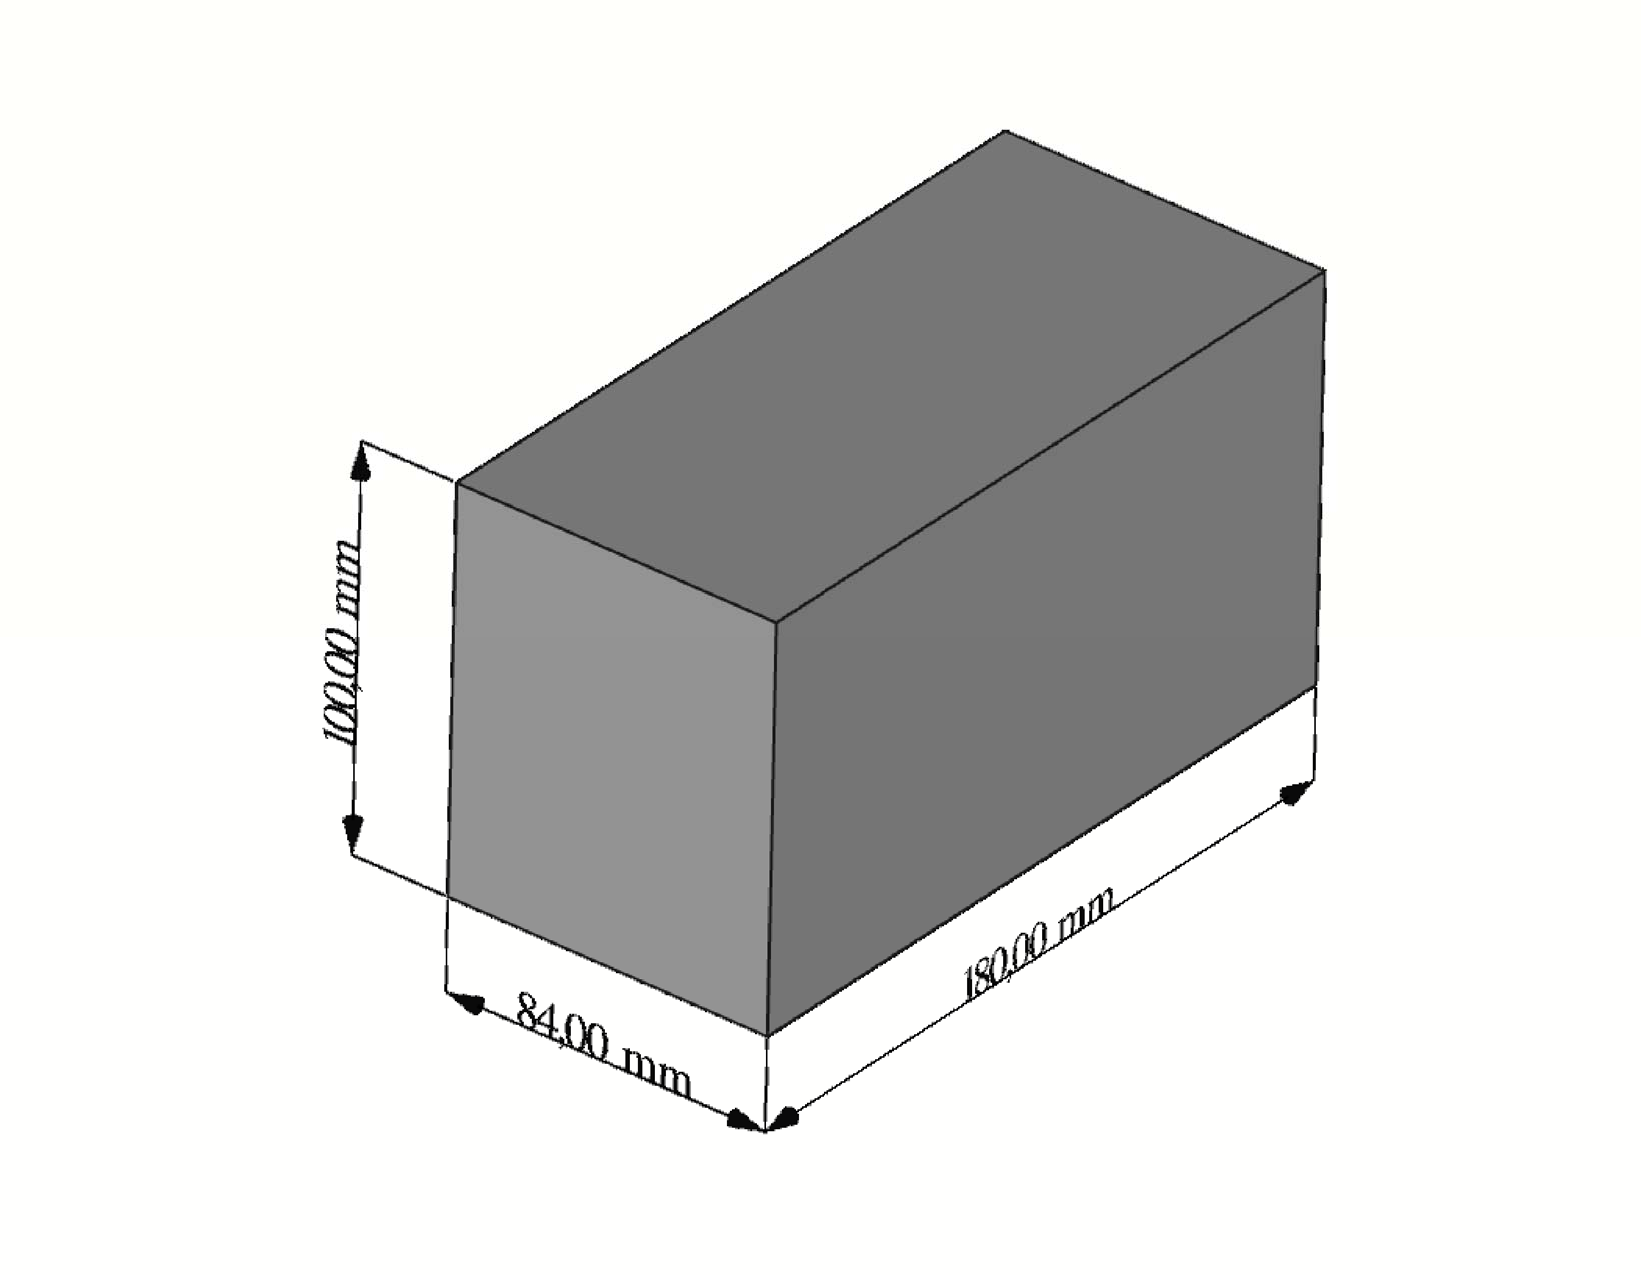
\includegraphics[scale=0.35]{./Resources/estLup/caixa_lupulos(1).pdf}
	\captionsetup{justification=centering}
	\caption[Dimens�es da estrutura de adi��o de l�pulos]{Dimens�es da estrutura de adi��o de l�pulos}
	\label{caixa_cinza}
\end{figure}

\begin{figure}[H]
	\centering
	\begin{subfigure}{.46\textwidth}
		\centering
		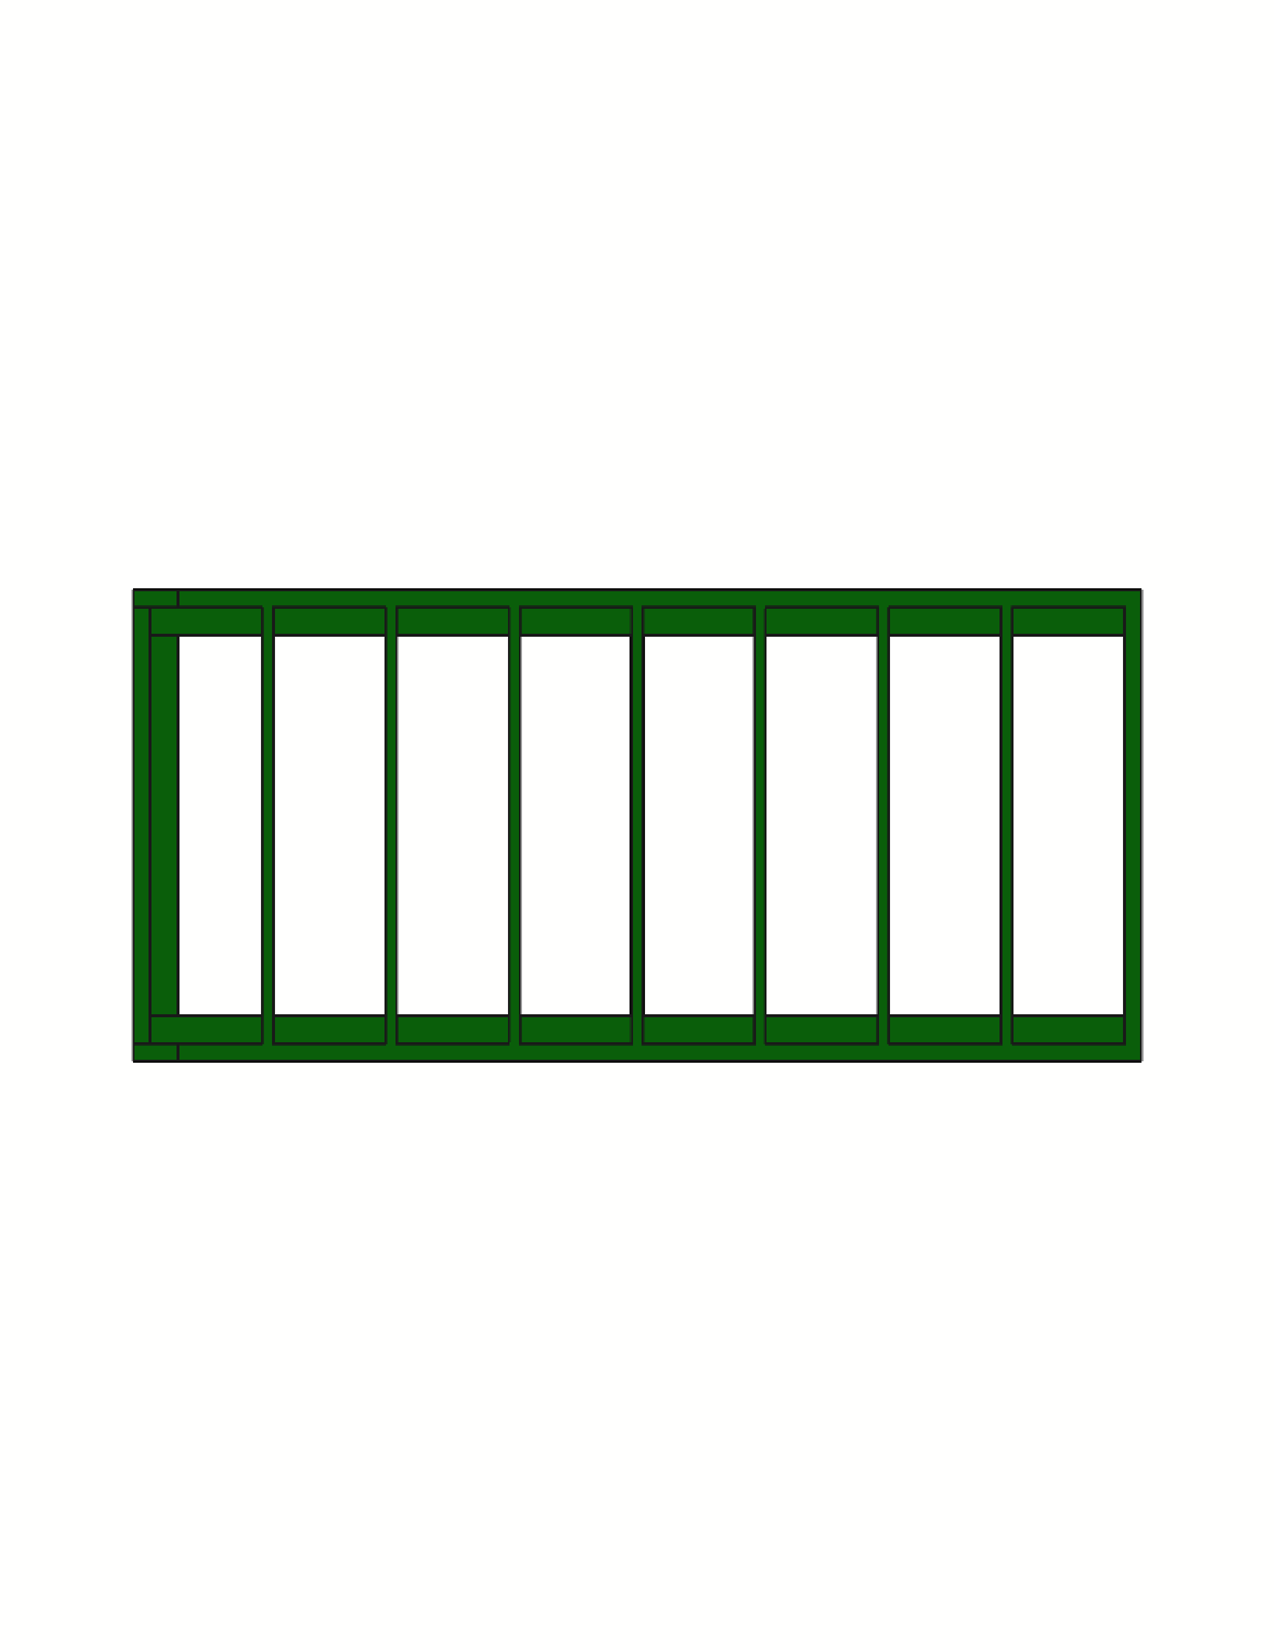
\includegraphics[height=7.5cm]{./Resources/estLup/caixa_lupulos(2).pdf}
		\caption{Vista superior}
		\label{corpo_hopbox:1}
	\end{subfigure}
	\begin{subfigure}{.46\textwidth}
		\centering
		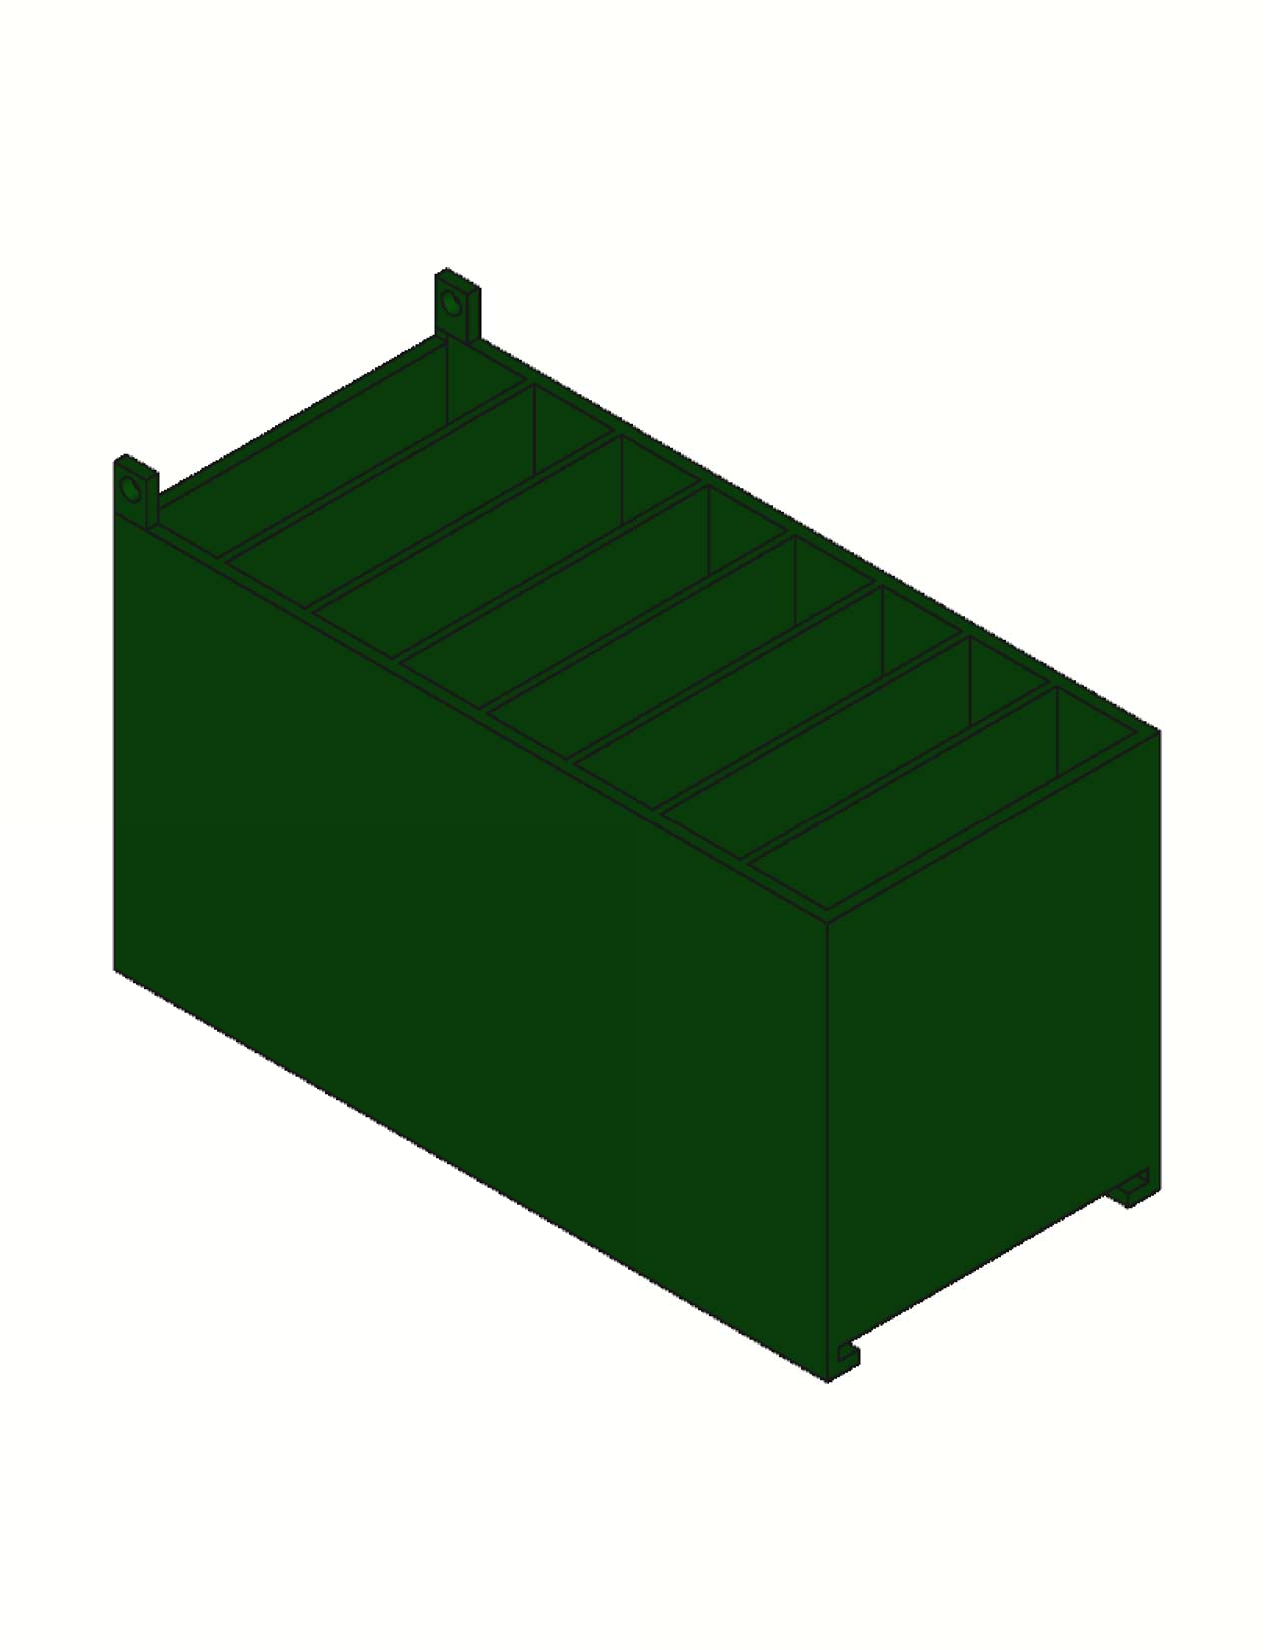
\includegraphics[height=7.5cm]{./Resources/estLup/caixa_lupulos(3).pdf}
		\caption{Vista axiom�trica}
		\label{corpo_hopbox:2}
	\end{subfigure}
	\captionsetup{justification=centering}
	\caption[Corpo da estrutura de adi��o de l�pulos]{Corpo da estrutura de adi��o de l�pulos}
	\label{corpo_hopbox}
\end{figure}

Foram projetadas duas portinholas: uma na face superior da caixa, para reabastecimento manual dos l�pulos, com uma al�a e fixada na caixa por dois pinos, de modo que a abertura desta tampa � um movimento de rota��o e; uma na face inferior, para adi��o autom�tica, de correr, de modo que a abertura � um movimento de transla��o; ambas est�o ilustradas na figura \ref{tampas_hopbox}.

\begin{figure}[H]
	\centering
	\begin{subfigure}{.46\textwidth}
		\centering
		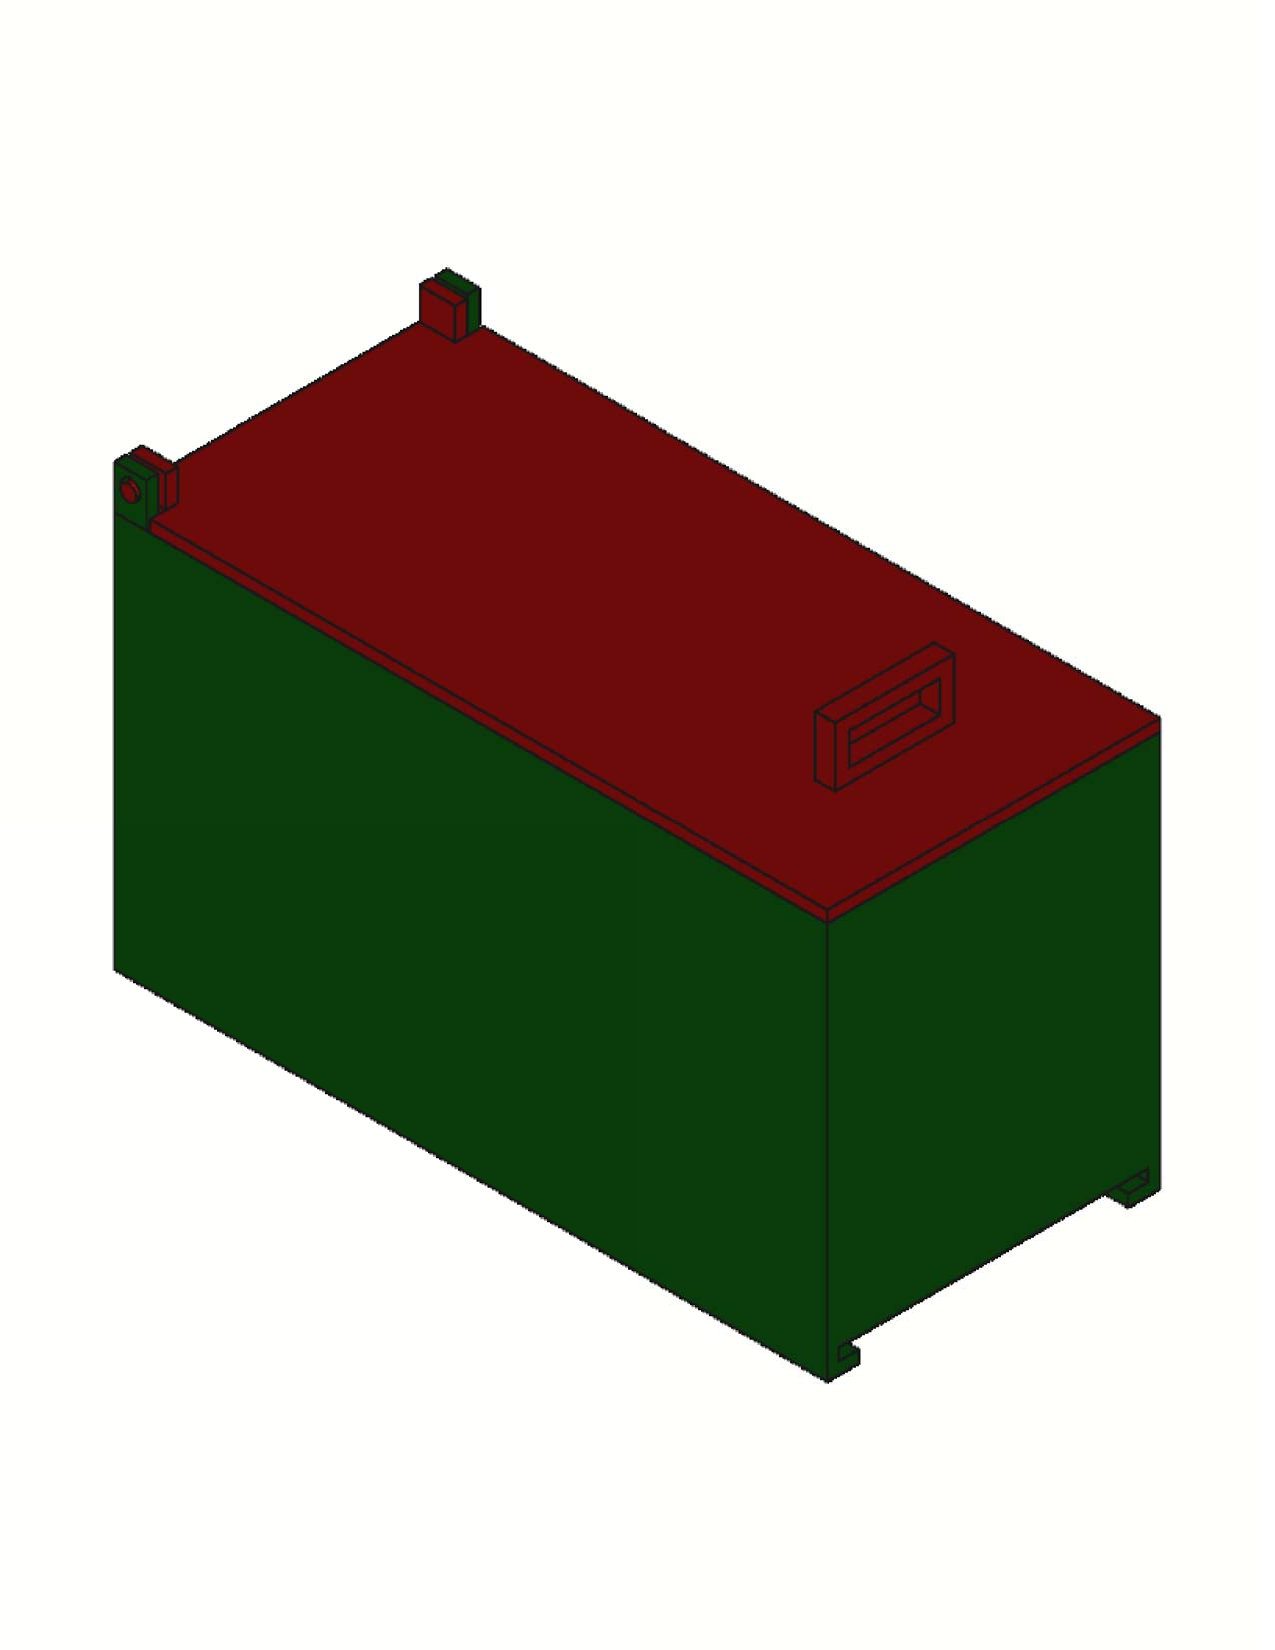
\includegraphics[height=7.5cm]{./Resources/estLup/caixa_lupulos(4).pdf}
		\caption{Tampa manual para reabastecimento}
		\label{tampas_hopbox:1}
	\end{subfigure}
	\begin{subfigure}{.46\textwidth}
		\centering
		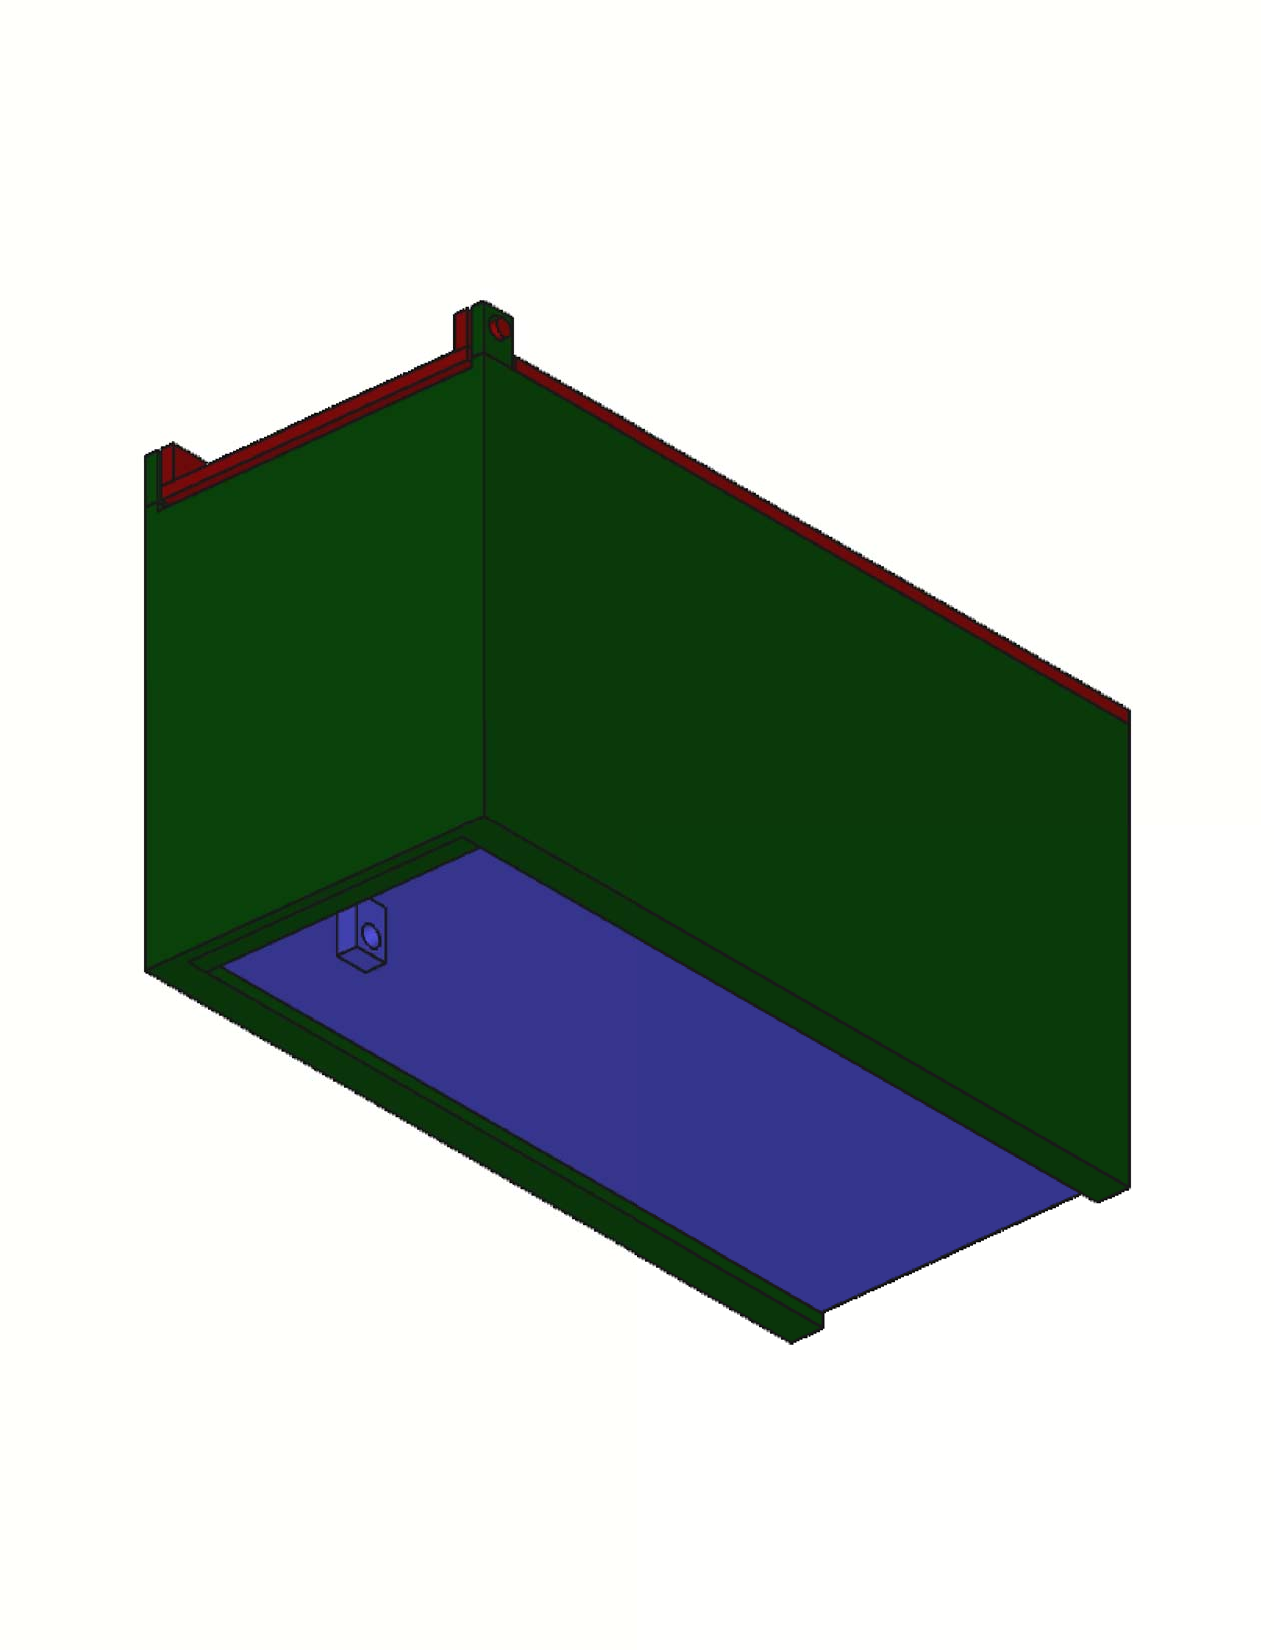
\includegraphics[height=7.5cm]{./Resources/estLup/caixa_lupulos(5).pdf}
		\caption{Tampa para adi��o autom�tica dos l�pulos}
		\label{tampas_hopbox:2}
	\end{subfigure}
	\captionsetup{justification=centering}
	\caption[Tampas da estrutura de adi��o de l�pulos]{Tampas da estrutura de adi��o de l�pulos}
	\label{tampas_hopbox}
\end{figure}

Duas varetas de comprimento $l_1$ e $l_2$ s�o ligadas ao encaixa da tampa de correr, representada em azul na figura \ref{tampas_hopbox:2}, e a elas � acoplado um servo-motor cujo �ngulo de opera��o $\theta$ define a abertura --- ou deslocamento --- da tampa, definido por $d$. A figura \ref{varetas} esquematiza as liga��es.

\begin{figure}[H]
	\centering
	\includegraphics[scale=0.1]{./Resources/estLup/esquema-varetas.jpg}
	\captionsetup{justification=centering}
	\caption[Esquema de liga��o das varetas � tampa de correr]{Esquema de liga��o das varetas � tampa de correr}
	\label{varetas}
\end{figure}

Sendo o comprimento da tampa igual a $l_3$, a condi��o em \ref{eq_varetas} deve ser satisfeita para que a excurs�o m�xima de abertura da caixa possa ser atingida. � poss�vel demonstrar com o aux�lio da Lei dos Cossenos, em \ref{eq_cossenos} que $l_1 = l_2 = l$ para que a m�nima abertura da caixa possa ser atingida.

\begin{align}
	\label{eq_varetas}
	l_1 + l_2 \geq l_3
\end{align}

\begin{align}
	\label{eq_cossenos}
	&l_2^2 = d^2 + l_1^2 - 2dl_1\cdot cos(\theta) \\
	&se \quad \theta = 90\si{\degree} \rightarrow d = 0 \therefore \nonumber\\
	\label{res_cossenos}
	&l_2^2 = l_1^2 \rightarrow l_2 = l_1 = l
\end{align}

A taxa m�xima de deslocamento em fun��o do �ngulo do servo motor � expressa em \ref{eq_desl}:

\begin{align}
	\label{eq_desl}
	\frac{dl_3}{d\theta} = \frac{2l}{90\si{\degree}}
\end{align}

Entretanto, quanto maior o valor desta taxa, menor � a resolu��o de abertura da caixa, portanto obtem-se que o menor valor poss�vel de $l$, a partir de \ref{eq_varetas} � $l = l_3/2$. Assim sendo, a taxa de deslocamento calculada a partir de \ref{eq_desl} � de $2mm/\si{\degree}$.

Embora o valor te�rico de $\theta$ seja $90\si{\degree}$, na pr�tica, devido ao encaixe entre tampa e vareta n�o ser na extremidade, este valor � reduzido. Tal fato n�o deve ser negligenciado, uma vez que isto pode for�ar a opera��o do servo-motor. Sabe-se pelo projeto executado no FreeCAD que a dist�ncia da borda ao encaixe da tampa � de 2,3cm portanto, com o aux�lio da Lei dos Cossenos, obt�m-se que $\theta_{max} = 82\si{\degree}$. Quanto ao valor m�nimo n�o h� preocupa��o , j� que a abertura da caixa ter� uma excurs�o reduzida em 2,3cm com rela��o ao seu comprimento. As varetas n�o foram calculadas novamente pois julgou-se uma boa pr�tica essa redu��o, que evita que a tampa caia da caixa quando em m�xima excurs�o. A figura \ref{completa_hopbox} apresenta o esquema completo de constru��o da estrutura de adi��o de l�pulos.

\begin{figure}[H]
	\centering
	\includegraphics[scale=0.25]{./Resources/estLup/final.jpg}
	\captionsetup{justification=centering}
	\caption[Estrutura de adi��o de l�pulos]{Estrutura de adi��o de l�pulos}
	\label{completa_hopbox}
\end{figure}

%%%%%%%%%%%%%%%%%%%%%%%%%%%%%%%%%%%%%%%%%%%%%%%%%%%%%%%%%%%%%%%%%%%%%%%%%%

\section{Configura��o da BeagleBone Black}

O primeiro passo para o desenvolvimento do projeto foi a configura��o da BeagleBone Black, que � o cora��o deste sistema. Para tal, foi escolhido o procedimento de gravar a distribui��o Debian pr�-compilada do sistema operacional Linux na mem�ria de armazenamento eMMC de 4GB da placa. Esta distribui��o foi escolhida em fun��o da facilidade de obten��o de suporte em f�runs da internet, artigos e livros, dentre outros, al�m de ser o SO oficial da BBB \cite{bbb_debian}.

NOTA: Na ocasi�o da realiza��o deste procedimento, havia uma diferencia��o entre a imagem fornecida para uso diretamente a partir do cart�o \si{\micro}SD e a imagem para grava��o no eMMC, por�m agora o procedimento adotado pela funda��o BeagleBoard.org � fornecer somente uma imagem pronta para uso diretamente do cart�o \si{\micro}SD e, no caso de o usu�rio decidir gravar a distribui��o no eMMC, o arquivo uEnv.txt na parti��o de \textit{boot} do cart�o \si{\micro}SD deve ser editado conforme instru��es antes de ser inserido na BBB.

Tanto a �ltima vers�o est�vel do Debian para BBB (v. 7.9), conhecida como \textit{Wheezy} e a �ltima vers�o em desenvolvimento (v. 8.2), conhecida como \textit{Jessie}, quanto a vers�o utilizada neste projeto (v. 7.5) podem ser obtidas a partir do site oficial da BBB \cite{bbb_images}, conforme ilustrado na figura \ref{debian_images}. A instala��o da vers�o 7.5 se resume a:

\begin{enumerate}
	\item Baixar a imagem Debian 7.5 para eMMC do site \url{beagleboard.org/latest-images}
	\item Descomprimir a imagem
	\item Gravar a imagem em um cart�o \si{\micro}SD formatado (n�o basta copiar, � preciso utilizar um software que grave a imagem corretamente. Neste caso foi utilizado o \textit{Win32 Disk Imager})
	\item Inserir o cart�o \si{\micro}SD na BBB desligada
	\item Pressionar o bot�o de boot e energizar a placa com ele ainda pressionado
	\item Esperar um dos leds de status acender antes de largar o bot�o
	\item Esperar os 4 leds de status ficarem continuamente acesos (durante o processo de grava��o eles trabalhar�o de maneira intermitente)
	\item Desenergizar a BBB e retirar o cart�o \si{\micro}SD
\end{enumerate}
 
 \newpage
 
\begin{figure}[H]
	\centering
	\fbox{\includegraphics[scale=0.30]{./Resources/debian-latest.jpg}}
	\captionsetup{justification=centering}
	\caption[�ltimas imagens pr�-compiladas dispon�veis para a BBB]{�ltimas imagens pr�-compiladas dispon�veis para a BBB. \\Fonte: Adaptado do site oficial da Funda��o BeagleBoard.org\protect\footnotemark}
	\label{debian_images}
\end{figure}

\footnotetext{Dispon�vel em \url{http://beagleboard.org/latest-images}}

Ap�s este procedimento, a BBB estar� pronta para uso a partir da mem�ria interna eMMC. A verifica��o do funcionamento do sistema foi feita conectando a placa a um computador instalado com Windows 7 e conectado � internet, via interface USB e posterior acesso atrav�s do software de c�digo aberto para acesso via SSH \textit{Putty}, dispon�vel para \textit{download} no site oficial \url{putty.org} \cite{putty} (qualquer software similar que possibilite o acesso via SSH pode ser utilizado para este fim). Para isso, � preciso tamb�m instalar no computador o driver que d� acesso � BBB via USB, dispon�vel em \url{beagleboard.org/getting-started}. O acesso via SSH se d� utilizando o endere�o de IP \textbf{192.168.7.2}, usu�rio: \textbf{debian} e senha: \textbf{debian} \cite{lumme}. A figura \ref{putty-cfg} mostra o ambiente de configura��o do \textit{Putty} e a figura \ref{putty-flogin} apresenta a tela ap�s uma tentativa de login bem sucedida.

\begin{figure}[H]
	\centering
	\includegraphics[scale=0.90]{./Resources/putty-cfg.jpg}
	\captionsetup{justification=centering}
	\caption[Configura��o do \textit{Putty} para acesso SSH via USB]{Configura��o do \textit{Putty} para acesso SSH via USB}
	\label{putty-cfg}
\end{figure}

\begin{figure}[H]
	\centering
	\includegraphics[scale=0.80]{./Resources/putty-first-login.jpg}
	\captionsetup{justification=centering}
	\caption[Tentativa de login bem sucedida pelo \textit{Putty}]{Tentativa de login bem sucedida pelo \textit{Putty}}
	\label{putty-flogin}
\end{figure}

\subsection{Ajustes de rede para uso do adaptador Wi-Fi/USB}

Para utilizar o adaptador Wi-Fi USB, em primeiro lugar este foi conectado � BBB. Em seguida, no terminal, o dispositivo foi listado para confirmar que o sistema estava identificando-o corretamente e ativado, permitindo assim obter a lista de redes Wi-Fi pr�ximas. Com isso, foi poss�vel obter os dados da rede Wi-Fi de interesse, para posterior edi��o do arquivo \textit{/etc/network/interfaces}, respons�vel pelas configura��es de rede do sistema -- este pode ser obtido no ap�ndice \ref{Ap�ndice B}. O c�digo \ref{wifi_conf} ilustra a sequ�ncia de comandos executados:

\lstset{language=bash}
\begin{lstlisting}[frame=single, basicstyle=\linespread{0.85}\ttfamily, caption=Passos para configura��o do Wi-Fi, label=wifi_conf]
lsusb # verifica se o dispositivo USB foi detectado
sudo ifconfig wlan up # ativa a interface de rede USB
sudo iwlist scan # lista as redes Wi-Fi dispon�veis

# Identificar os valores da rede de interesse, e.g.
#	ESSID:"Nome_da_rede" -> nome da rede
#	IE: IEEE 802.11i/WPA2 Version 1 -> encripta��o
# E ent�o � modificado o arquivo de configura��o

# abre o arquivo para edi��o
sudo nano /etc/network/interfaces 
# Ap�s modificar o arquivo e salv�-lo:

sudo ifup wlan0 # ativa a interface de rede Wi-Fi
sudo ifdown eth0 # desativa a interaface Ethernet

\end{lstlisting}

No arquivo \textit{/etc/network/interfaces}, as configura��es utilizadas entre as linhas 19 e 35 do c�digo s�o referentes � configura��o do Wi-Fi para configura��o da BBB com endere�o de IP est�tico 192.168.1.155, permitindo o acesso � plataforma remotamente pela internet e n�o somente dentro da intranet. Observe-se que o acesso a este IP da intranet se d� pelo IP externo 143.107.xxx.xxx, que � o endere�o do departamento da engenharia el�trica da USP de S�o Carlos. Por motivos de seguran�a este ser� omitido no presente trabalho.

Depois de todo este procedimento, o dispositivo ainda n�o estava funcionando ap�s a opera��o de \textit{reboot}, portanto foi utilizado um \textit{script} de reset do Wi-Fi executado durante o \textit{boot}, cujas instru��es de uso, obtidas em  \url{https://learn.adafruit.com/setting-up-wifi-with-beaglebone-black/configuration}, est�o descritas no c�digo-fonte \ref{rst_wifi}. A figura \ref{success_ssh} indica sucesso de conex�o via SSH usando uma m�quina com sistema operacional Linux Ubuntu 14.04 LTS.

\lstset{language=bash}
\begin{lstlisting}[frame=single, basicstyle=\linespread{0.85}\ttfamily, caption=Configura��o para reset do Wi-Fi ap�s o boot, label=rst_wifi]
git clone https://github.com/adafruit/wifi-reset.git #download do script
cd wifi-reset/ #entra no diret�rio do script
chmod +x install.sh #permiss�o de execu��o para o script
sudo ./install.sh #executa o script
\end{lstlisting}

\begin{figure}[H]
	\centering
	\includegraphics[scale=0.50]{./Resources/ssh_login_linux.jpg}
	\captionsetup{justification=centering}
	\caption[Acesso � BBB via SSH]{Acesso � BBB via SSH}
	\label{success_ssh}
\end{figure}

\subsection{Data/hora}

Para a configura��o autom�tica de data e hora da BBB, foi escolhido o uso do protocolo NTP -- \textit{Network Time Protocol} ou Protocolo de Tempo para Redes -- cujo objetivo � sincronizar os rel�gios de dispositivos conectados a uma rede a partir de fontes precisas \cite{ntp}. No Brasil, a confiabilidade deste protocolo � responsabilidade do Observat�rio Nacional (ON), respons�vel legal por garantir a Hora Legal Brasileira, em conjunto com o N�cleo de Informa��o e Coordena��o do Ponto BR, administrador e operador do dom�nio ".br"  \cite{nic,dsho}.

Primeiramente foi realizada a instala��o do protocolo, seguida da configura��o do arquivo \textit{/etc/ntp.conf} e da modifica��o do arquivo que indica a \textit{timezone}, sendo este um link simb�lico para o verdadeiro arquivo. Os comandos executados est�o descritos no c�digo-fonte \ref{ntp_install}:

\lstset{language=bash}
\begin{lstlisting}[frame=single, basicstyle=\linespread{0.85}\ttfamily, caption=Instala��o e configura��o do NTP, label=ntp_install]
sudo apt-get install ntp #instala o NTP
sudo nano /etc/ntp.conf #abre o arquivo de configura��o para edi��o
sudo mv /etc/localtime /etc/localtime-old #backup do arquivo antigo da timezone
sudo ln -s /usr/share/zoneinfo/America/Sao_Paulo /etc/localtime #cria link simb�lico para arquivo da nova timezone
\end{lstlisting}

Na edi��o do arquivo \textit{/etc/ntp.conf}, a �nica modifica��o feita � a substitui��o dos servidores de hora padr�o para os servidores brasileiros, listados no endere�o \url{http://www.pool.ntp.org/zone/br} -- no final de cada endere�o foi adicionada a instru��o \textit{iburst}, conforme descrito no website oficial do protocolo (\url{http://support.ntp.org/bin/view/Support/ConfiguringNTP}) e que, embora n�o esteja claro seu funcionamento, � essencial para que o hor�rio seja corretamente configurado a cada \textit{reboot}. O trecho de c�digo-fonte \ref{ntp_br} indica as modifica��es no arquivo \textit{/etc/ntp.conf} adequando aos servidores brasileiros:

\lstset{language=bash}
\begin{lstlisting}[frame=single, basicstyle=\linespread{0.85}\ttfamily, caption=Servidores brasileiros do NTP, label=ntp_br]
# You do need to talk to an NTP server or two (or three).
#server ntp.your-provider.example

# pool.ntp.org maps to about 1000 low-stratum NTP servers. Your server will
# pick a different set every time it starts up. Please consider joining the
# pool: <http://www.pool.ntp.org/join.html>
server 0.br.pool.ntp.org iburst
server 1.br.pool.ntp.org iburst
server 2.br.pool.ntp.org iburst
server 3.br.pool.ntp.org iburst
\end{lstlisting}

\subsection{Sensor DS18B20}

Uma vez que o sensor de temperatura DS18B20 j� � suportado pelo Kernel e inclu�do como \textit{driver} na distribui��o padr�o da BBB, somente foi necess�rio criar uma sobreposi��o de \textit{device tree} indicando em que pino o sensor est� ligado. Tanto o mux quanto o OCP do SoC precisaram ser configurados e, para a compila��o do arquivo texto em bin�rio, foi necess�ria a instala��o do DTC, descrita no c�digo-fonte \ref{dtc_install}:

\lstset{language=bash}
\begin{lstlisting}[frame=single, basicstyle=\linespread{0.85}\ttfamily, caption=Instala��o do DTC, label=dtc_install]
sudo wget -c https://raw.github.com/RobertCNelson/tools/master/pkgs/dtc.sh 
sudo chmod +x dtc.sh
./dtc.sh
\end{lstlisting}

O arquivo com a sobreposi��o da \textit{device tree} � descrito na se��o \ref{ap3ds18b20}, por�m o c�digo-fonte \ref{dtf_ds18b20} apresenta um trecho relevante deste, no qual observa-se a configura��o do multiplexador do SoC. Note-se que esta configura��o significa que o \textit{pull-up} interno de 10k\ohm da BBB est� ativado, eliminando a necessidade de um resistor externo. O valor m�nimo de \textit{pull-up} segundo a folha de dados do sensor � de 4,7k\ohm, mas n�o foi observada perda de desempenho do mesmo na presente configura��o.

\lstset{language=bash}
\begin{lstlisting}[frame=single, basicstyle=\linespread{0.85}\ttfamily, caption=Fragmento de device tree para o DS18B20, label=dtf_ds18b20]
bb_w1_pins: pinmux_bb_w1_pins {
	pinctrl-single,pins =  <0x70 0x37>;
};
\end{lstlisting}

A compila��o da sobreposi��o � executada com o comando presente no trecho de c�digo \ref{dtc_compile}. Adicionar "-00A0" ao nome do arquivo de sa�da DTBO � fundamental. Note-se tamb�m que o arquivo DTBO � copiado para o diret�rio no qual ficam todas as sobreposi��es de \textit{device tree}. Para carregar a sobreposi��o no boot, � preciso adicionar a linha \textit{echo w1 > /sys/devices/bone\_capemgr.*/slots} ao arquivo \textit{/etc/rc.local}.

\lstset{language=bash}
\begin{lstlisting}[frame=single, basicstyle=\linespread{0.85}\ttfamily, caption=Compila��o de \textit{device tree}, label=dtc_compile]
sudo dtc -O dtb -o w1-00A0.dtbo -b 0 -@ w1.dts
sudo cp w1-00A0.dtbo /lib/firmware
\end{lstlisting}

Ap�s o reboot e com o sensor conectado � BBB, � poss�vel obter o valor da temperatura realizando a leitura do arquivo \textit{/sys/devices/w1\_bus\_master1/28-*/w1\_slave}, conforme ilustrado na figura \ref{ds_reading}. Observe-se que na figura ao inv�s do asterisco foi utilizado o identificador �nico deste sensor espec�fico --- quando � utilizado um asterisco, ele � substitu�do por todos os poss�veis nomes de sensores, portanto � �til para leitura de diversos sensores de uma vez. Para saber quantos dispositivos com o protocolo \textit{1-wire} est�o conectados � mesma linha e assim descobrir os n�meros referentes a eles, � poss�vel ler o arquivo \textit{/sys/devices/w1\_bus\_master1/w1\_master\_slaves} ou ent�o verificar o conte�do do diret�rio \textit{/sys/devices/w1\_bus\_master1/}.

\begin{figure}[H]
	\centering
	\includegraphics[scale=0.50]{./Resources/ds_reading_terminal.jpg}
	\captionsetup{justification=centering}
	\caption[Leitura do sensor DS18B20 pelo terminal]{Leitura do sensor DS18B20 pelo terminal}
	\label{ds_reading}
\end{figure}

\subsection{Webserver Apache}

Embora o Apache venha instalado na distribui��o padr�o da imagem do Debian para a BBB, � preciso configurar a porta que ele usa para conex�es, predefinida pelas configura��es de rede do departamento de engenharia el�trica. A porta ser� omitida por seguran�a, mas na descri��o do processo de configura��o aqui proposta ser� usado o valor 8080, padr�o para diversos protocolos de internet, inclusive o HTTP.

H� dois arquivos que devem ser editados para modificar as configura��es do Apache. No arquivo \textit{/etc/apache2/sites-enabled/000-default} a primeira linha do arquivo deve ser modificada para \textit{<VirtualHost *:8080>} e no arquivo \textit{/etc/apache2/ports.conf} as linhas \textit{NameVirtualHost *:8080} e \textit{Listen 8080} devem ser adicionadas ou modificadas, caso j� existam. Para que as configura��es tenham efeito, o servidor deve ser reiniciado com o comando descrito na caixa de c�digo-fonte \ref{restart_apache}:

\lstset{language=bash}
\begin{lstlisting}[frame=single, basicstyle=\linespread{0.85}\ttfamily, caption=Reinicializa��o do servidor web Apache, label=restart_apache]
sudo service apache2 restart
\end{lstlisting}


%%%%%%%%%%%%%%%%%%%%%%%%%%%%%%%%%%%%%%%%%%%%%%%%%%%%%%%%%%%%%%%%%%%%%%%%%%

\section{IDE e sistema de controle de vers�o}

\subsection{\textit{Cloud9}}

\subsection{\textit{GitHub}}

%%%%%%%%%%%%%%%%%%%%%%%%%%%%%%%%%%%%%%%%%%%%%%%%%%%%%%%%%%%%%%%%%%%%%%%%%%

\section{Gera��o de gr�fico e registro de temperatura em Python}

Para o armazenamento da temperatura do sensor em fun��o do tempo, assim como a gera��o de um gr�fico com o hist�rico de temperaturas para o usu�rio do sistema, foram escritos dois \textit{scripts} em Python, sendo a sa�da do \textit{script} de \textit{log} a entrada do \textit{script} de gera��o do gr�fico --- embora ambos possam ser executados independentemente, a gera��o do gr�fico precisa de um arquivo contendo o hist�rico de temperaturas.

\subsection{Registro de temperatura}

Para o arquivo do \textit{log}, foram primeiramente escritas algumas fun��es:

\begin{itemize}
	\item \textbf{tread()} --- l� o arquivo referente ao sensor de temperatura e retorna deste somente a temperatura formatada em graus celsius.
	\item \textbf{tprint\_all(tcelsius)} ---  recebe temperatura em \si{\degree}C e imprime com formata��o HTML em \si{\degree}C, \si{\degree}F, K e \si{\degree}R; pode ser usada em conjunto com a fun��o tread()
	\item \textbf{tprint\_all\_terminal(tcelsius)} ---  id�ntica � fun��o tprint\_all(), por�m imprime com formata��o
para o terminal do Linux
	\item \textbf{tlog(file = "/var/www/default.csv")} --- cria/adiciona a um arquivo de log no formato CSV a
temperatura medida e a data/hora correspondente no formato \textit{Unix epoch} --- que � definido como o n�mero de segundos passados desde 1 de janeiro de 1970 n�o considerando segundos bissextos --- em intervalo de amostragem definido na fun��o, at� que o script seja interrompido de alguma maneira. Em fun��o de erros de leitura espor�dicos do sensor, se a temperatura lida for menor ou igual a zero, esta � descartada. Imprime a temperatura lida a cada amostragem. O tempo de amostragem � definido pela soma do tempo de leitura do arquivo (inerente ao sistema) com o tempo ocioso definido nesta fun��o: para que o tempo de amostragem seja o mais pr�ximo poss�vel de 1s, foi realizado um estudo de caso, descrito no ap�ndice \ref{analise_tread_temp}, e com isso obteve-se o valor de 0,2202s ocioso definido nesta fun��o. Al�m disto, nesta fun��o � chamada \textit{tlog\_instant} que registra em um arquivo separado a �ltima leitura v�lida de temperatura e tempo.
	\item \textbf{tlog\_instant(temperature, epoch, file = "/var/www/datalog/instant.csv")} --- registra a �ltima leitura v�lida de temperatura e tempo em um arquivo, criando ou sobrescrevendo o mesmo.
	\item \textbf{tlog\_test(file = "/var/www/datalog/default.csv")} --- fun��o que gera um arquivo de \textit{log} com rampas e degraus de temperatura, para uso em simula��es posteriores do funcionamento do sistema, descritas na se��o \ref{simulacao_controle}.
\end{itemize}

Sendo a fun��o \textit{tlog} a mais relevante, esta pode ser obtida na caixa de c�digo-fonte \ref{tlog_python}. O script completo est� registrado no c�digo-fonte \ref{python_log_script} do ap�ndice \ref{codigos_python}. Ainda assim, as fun��es por si s� n�o s�o executadas sozinhas, portanto foi criado um script auxiliar em Python que chama a fun��o \textit{tlog}, descrito no c�digo-fonte \ref{tlog_log}.

\lstset{language=Python}
\begin{lstlisting}[frame=single, basicstyle=\linespread{0.85}\ttfamily, caption=Fun��o de \textit{log} da temperatura em Python, label=tlog_python]
def tlog(file = "/var/www/datalog/default.csv"):
	"""salva temperatura e Unix Time em .csv """
	tsample = 0.2202 #amostra a cada ~1 segundo
	buff_temp = tread()#guarda o �ltimo valor lido
	exist = os.path.isfile(file)
	with open(file, 'a', 1) as log:
		if exist is False:#se vai criar o arquivo agora
			log.write("temperatura,data\n")
		while True: #loop infinito
			temp_celsius = tread()
			epoch = time.time()#l� a data/hora do sistema
			if temp_celsius >= 0:#evita leitura errada
				log.write("%f,%f\n" % (temp_celsius, epoch))
				tlog_instant(temp_celsius, epoch)
				time.sleep(tsample)#espera n segundos
				print "registrando temperatura!",temp_celsius
\end{lstlisting}

\lstset{language=Python}
\begin{lstlisting}[frame=single, basicstyle=\linespread{0.85}\ttfamily, caption=Script para grava��o das leituras de temperatura em Python, label=tlog_log]
import temp
temp.tlog()
# para executar no terminal, basta executar:
# sudo python log.py
\end{lstlisting}

Na figura \ref{csv_log_example} � apresentada uma amostra de arquivo CSV gerado pelo script \ref{tlog_log}.

\begin{figure}[H]
	\centering
	\includegraphics[scale=0.50]{./Resources/csv_log_example.jpg}
	\captionsetup{justification=centering}
	\caption[Arquivo CSV com registro de temperaturas gerado em Python]{Arquivo CSV com registro de temperaturas gerado em Python}
	\label{csv_log_example}
\end{figure}

\subsection{Gr�fico de temperatura}

\section{Aplica��o \textit{server-side} em Node.js}

\subsection{Servidor Express.js}

\subsection{Projeto do controle do sistema}

\subsection{Simula��o do controle do sistema}
\label{simulacao_controle}
%%%%%%%%%%%%%%%%%%%%%%%%%%%%%%%%%%%%%%%%%%%%%%%%%%%%%%%%%%%%%%%%%%%%%%%%%%

\section{Interface de usu�rio}

A interface de usu�rio foi desenvolvida para acesso via navegador da internet. Dois servidores foram utilizados em conjunto: o servidor Apache, que � um servidor \textit{web} robusto e de f�cil implementa��o e o \textit{framework Express.js}, para \textit{Node.js}. As linguagens utilizadas para a implementa��o da aplica��o foram: a linguagem de marca��o HTML, a linguagem de folhas de estilo CSS, a linguagem de programa��o \textit{client-side} interpretada Javascript em conjunto com a biblioteca \textit{crossbrowser} jQuery e o m�todo AJAX, a linguagem de programa��o \textit{server-side} interpretada PHP e, a linguagem de programa��o \textit{server-side} Javascript interpretada pela aplica��o \textit{Node.js}.

Parte da implementa��o foi feita por meio de acesso ao terminal via SSH e parte via \textit{Cloud9}, que � uma IDE online. A estrutura da aplica��o desenvolvida � apresentada:

\begin{itemize}
	\item P�gina inicial
	\item P�gina de apresenta��o
	\item Gr�ficos de temperatura din�mico e est�tico (p�gina somente para vers�o de demonstra��o)
	\item Menu de sele��o de tarefas
	\begin{itemize}
		\item Gerenciador de receitas de cerveja
		\begin{itemize}
			\item Editor de receitas
		\end{itemize}
		\item Gerenciador de in�cio da produ��o (em desenvolvimento)
		\item Acompanhamento e possibilidade de ajustes da brassagem (em desenvolvimento)
		\item Estat�sticas (a ser desenvolvida)
		\item Op��es e ajuste de configura��es do sistema (a ser desenvolvida)
	\end{itemize}
\end{itemize}

Os c�digos desenvolvidos e comentados podem ser consultados no ap�ndice \ref{Ap�ndice B} e os resultados s�o descritos na se��o \ref{resIntUser}.

%%%%%%%%%%%%%%%%%%%%%%%%%%%%%%%%%%%%%%%%%%%%%%%%%%%%%%%%%%%%%%%%%%%%%%%%%%

\section{Circuitos de interface entre a BBB e sensores/atuadores}

\subsection{Acionamentos de pot�ncia}

\subsection{Detector de \textit{zero-crossing}}

\subsection{Detector de n�vel de l�quido}

%\subsection{mais o que?}

%%%%%%%%%%%%%%%%%%%%%%%%%%%%%%%%%%%%%%%%%%%%%%%%%%%%%%%%%%%%%%%%%%%%%%%%%%

\section{Sistema de controle de temperatura}

\subsection{Resistores de aquecimento}

\subsection{Controlador PID}


\chapter{Resultados e Discuss�es}
\label{Resultados}

Neste cap�tulo s�o apresentados os resultados obtidos a partir dos m�todos descritos na se��o \ref{Materiais}.

%%%%%%%%%%%%%%%%%%%%%%%%%%%%%%%%%%%%%%%%%%%%%%%%%%%%%%%%%%%%%%%%%%%%

\section{Interface de usu�rio}
\label{resIntUser}

Nesta se��o s�o apresentados os resultados do desenvolvimento da interface de usu�rio. 

A p�gina inicial � composta de uma imagem com uma �rea clic�vel no centro, sobre a etiqueta \textit{Start Here}, que leva � p�gina de apresenta��o. O resultado visual de seu desenvolvimento pode ser verificado na figura \ref{ui-ini}.

\begin{figure}[H]
	\centering
	\includegraphics[scale=0.90]{./Resources/uips/inipg.jpg}
	\captionsetup{justification=centering}
	\caption{P�gina inicial da UI}
	\label{ui-ini}
\end{figure}

A p�gina de apresenta��o cont�m uma breve descri��o do projeto e de seu objetivo, al�m dos bot�es que levam: � interface onde est�o os gr�ficos de temperatura e; ao menu de sele��o de tarefas. O resultado visual de seu desenvolvimento pode ser verificado na figura \ref{ui-present}.

\begin{figure}[H]
	\centering
	\includegraphics[scale=0.90]{./Resources/uips/presentpg.jpg}
	\captionsetup{justification=centering}
	\caption{P�gina de apresenta��o da UI}
	\label{ui-present}
\end{figure}

Na p�gina que plota os gr�ficos de temperatura em fun��o do tempo � poss�vel ler o valor atual da temperatura do sensor DS18B20. Tamb�m � nesta p�gina que encontra-se o gr�fico din�mico e interativo, que � atualizado a cada aproximadamente 1 segundo -- o tempo de atualiza��o n�o � fixo em fun��o da natureza de opera��o do interpretador do Javascript e o tempo de amostragem da temperatura n�o � fixo em fun��o do sistema operacional escolhido n�o ser de tempo real. Neste gr�fico, apresentado na figura \ref{ui-graph1} � poss�vel:

\begin{itemize}
	\item Selecionar as vari�veis plotadas
	\item Escolher a plotagem do gr�fico em linha ou �rea
	\item Empilhar ou sobrepor os gr�ficos (no caso da plotagem em �rea)
	\item Unir os pontos amostrados em degrau, linha ou realizar uma interpola��o cardinal
	\item Suavizar a plotagem empregando um filtro de m�dia m�vel
	\item Escolher o n�mero de pontos plotados, de maneira a obter o registro dos �ltimos: 5 minutos, 30 minutos ou 1 hora de amostragens
	\item Ajuste fino do n�mero de pontos plotados, por meio da escolha dos limites inicial e final, utilizando a barra sob o gr�fico
	\item Leitura precisa do valor de qualquer ponto plotado e da data/hora da amostragem, colocando o cursor sobre o local do gr�fico no qual se deseja realizar a leitura
\end{itemize}

\begin{figure}[H]
	\centering
	\includegraphics[scale=0.90]{./Resources/uips/graphpg1.jpg}
	\captionsetup{justification=centering}
	\caption[Gr�fico din�mico de temperatura em fun��o do tempo]{Gr�fico din�mico de temperatura em fun��o do tempo \\ Ajuste fino e cursor sobre o gr�fico sendo aplicados}
	\label{ui-graph1}
\end{figure}

Ainda na p�gina que plota os gr�ficos de temperatura, � plotado um gr�fico est�tico do hist�rico de todos os pontos registrados no arquivo de \textit{log}. O resultado visual de seu desenvolvimento pode ser verificado na figura \ref{ui-graph2}.

\begin{figure}[H]
	\centering
	\includegraphics[scale=0.90]{./Resources/uips/graphpg2.jpg}
	\captionsetup{justification=centering}
	\caption{Gr�fico est�tico do hist�rico de temperaturas registradas}
	\label{ui-graph2}
\end{figure}

O menu de tarefas, ilustrado na figura \ref{ui-task} � basicamente uma p�gina com links para o gerenciador de receitas, o gerenciador de in�cio da produ��o, o acompanhamento e ajustes da brassagem e as estat�sticas. A p�gina de configura��es e op��es n�o foi implementada em tempo.

\begin{figure}[H]
	\centering
	\includegraphics[scale=0.90]{./Resources/uips/taskmenupg.jpg}
	\captionsetup{justification=centering}
	\caption{Menu de tarefas da UI}
	\label{ui-task}
\end{figure}

O gerenciador de receitas lista e permite acesso a todas as receitas cadastradas no sistema, possibilita exclus�o (com a op��o de desfazer para exclus�o acidental) e cria��o de nova receita. Quando o cursor � colocado sobre uma receita cadastrada, � apresentado um \textit{preview} para que o usu�rio tenha uma realimenta��o r�pida de seu conte�do. A figura \ref{ui-manager} ilustra esta interface em uso, com o cursor sobre a receita \textit{TheMightyMightyIPA} e seu \textit{preview}, al�m da receita \textit{Exemplo Kolsch} exclu�da e com possibilidade de recupera��o.

\begin{figure}[H]
	\centering
	\includegraphics[scale=0.90]{./Resources/uips/managerpg.jpg}
	\captionsetup{justification=centering}
	\caption[Gerenciador de receitas da UI]{Gerenciador de receitas da UI \\ Cursor sobre a receita \textit{TheMightyMightyIPA} e receita \textit{Exemplo Kolsch} exclu�da}
	\label{ui-manager}
\end{figure}

O editor de receitas apresenta caixas de entrada para o usu�rio adicionar as caracter�sticas desejadas da cerveja, sendo que a cada malte, l�pulo e temperatura adicionado, aparece automaticamente um campo extra para estes itens, limitado a 8 entradas para cada. S� foi implementado um bot�o de voltar pois h� uma funcionalidade de salvamento autom�tico -- o aviso no canto superior direito da tela mostra o status do salvamento da receita: no caso da figura \ref{ui-editor}, que ilustra a implementa��o do editor, nota-se que a mensagem de status avisa o usu�rio que h� um campo essencial para a produ��o da cerveja que n�o foi preenchido.

\begin{figure}[H]
	\centering
	\includegraphics[scale=0.90]{./Resources/uips/editorpg.jpg}
	\captionsetup{justification=centering}
	\caption[Editor de receitas da UI]{Editor de receitas da UI \\ Receita \textit{bla} parcialmente preenchida com aviso de campos essenciais em branco}
	\label{ui-editor}
\end{figure}

O gerenciador de in�cio da produ��o apresenta ao usu�rio um aviso sinalizando de que tudo deve estar devidamente verificado antes do in�cio da produ��o. Tamb�m apresenta uma caixa de sele��o da receita a ser produzida. O resultado visual de seu desenvolvimento pode ser verificado na figura \ref{ui-start}.

\begin{figure}[H]
	\centering
	\includegraphics[scale=0.90]{./Resources/uips/startbrewingpg.jpg}
	\captionsetup{justification=centering}
	\caption{Gerenciador de in�cio da produ��o}
	\label{ui-start}
\end{figure}

O acompanhamento e possibilidade de ajustes da brassagem implementa um controle manual do LED1 da BBB, bombas, v�lvulas, resistores de pot�ncia e servo-motor do sistema, com \textit{feedback} visual para o usu�rio. Na figura \ref{ui-ctrl} � apresentada a UI e o console do Javascript, no qual aparecem as respostas do servidor para a seguinte sequ�ncia de comandos: ativa��o da bomba do mosto, ativa��o da v�lvula da �gua, valor do �ngulo do servo-motor setado para 87\si{\degree} e, ativa��o seguida desligamento do aquecedor de fervura.

\begin{figure}[H]
	\centering
	\includegraphics[scale=0.90]{./Resources/uips/manualctrlpg.jpg}
	\captionsetup{justification=centering}
	\caption{Interface de acompanhamento e ajustes da brassagem - console Javascript com \textit{feedback} do servidor para uma sequ�ncia de comandos executados}
	\label{ui-ctrl}
\end{figure}


A p�gina de estat�sticas apresenta somente um aviso de p�gina em desenvolvimento, conforme ilustrado na figura \ref{ui-dev}.

\begin{figure}[H]
	\centering
	\includegraphics[scale=0.90]{./Resources/uips/developg.jpg}
	\captionsetup{justification=centering}
	\caption{Aviso de p�gina em desenvolvimento}
	\label{ui-dev}
\end{figure}
\chapter{Conclus�es}
\label{Conclusao}

Este cap�tulo � dedicado �s conclus�es levantadas a partir dos resultados obtidos para este trabalho de conclus�o de curso. No intuito de facilitar a organiza��o destas, o cap�tulo est� dividido em se��es nas quais se discorrem t�picos espec�ficos do projeto, buscando seguir a ordem do cap�tulo de resultados.

\section{Sistema de controle de vers�o}

Com rela��o ao sistema de controle de vers�o \textit{Git} e o servi�o online \textit{GitHub}, foi observado o poder que estas ferramentas proporcionam � documenta��o e manuten��o de um projeto que envolve \textit{software}. O simples fato de documentar cada mudan�a feita ao c�digo-fonte de maneira simples, no n�vel de detalhamento que o usu�rio considerar adequado, j� justificou o seu uso: este n�vel de documenta��o e sua facilidade s�o um dos pontos essenciais para a facilidade de documenta��o de c�digo, pois o desenvolvedor sabe o que foi modificado e quando gastando um m�nimo esfor�o.

A possibilidade de desenvolver esta monografia empregando o \textit{GitHub} como um meio de \textit{backup} e de ter os arquivos necess�rios dispon�veis em qualquer lugar tamb�m foi um dos pontos fortes observados que justificou o uso da ferramenta --- al�m de que os registros incrementais ajudaram a recuperar o racioc�nio em per�odos nos quais a escrita foi deixada em segundo plano em fun��o do desenvolvimento do projeto.

Embora tenha sido l�gico o resultado estat�stico do \textit{punchcard}, apresentado na se��o \ref{git_res} --- em fun��o de tarefas de maior prioridade executadas durante os dias �teis da semana, foi observado que o desenvolvimento do TCC se deu nos hor�rios livres --- � poss�vel extrapolar o uso desta ferramenta estat�stica no monitoramento de uma equipe de desenvolvimento de software, que n�o precisa necessariamente trabalhar em um mesmo local f�sico.

Por fim, com rela��o ao \textit{Git}, durante alguns momentos do projeto, foi constatado que apesar de a ferramenta ser excelente para o desenvolvimento de \textit{software}, em �ltima inst�ncia ela reflete a disciplina e o h�bito do programador no uso desta. Isto foi notado em momentos nos quais mudan�as simples, mas importantes para o c�digo-fonte, eram ignoradas no sentido de atualiz�-las no \textit{Git}. Outra quest�o importante com rela��o ao uso que se faz desta ferramenta � que, ao trabalhar em uma equipe, provavelmente seja melhor combinar com os colaboradores qual o n�vel de detalhamento desejado para a documenta��o e quais as t�cnicas de uso, e.g. criar uma ramifica��o para consertar um determinado bug ou somente para implementar uma nova funcionalidade, dentre outras possibilidades.

\section{Gera��o de gr�ficos e registro de temperatura em Python}

� importante notar que as duas aplica��es escritas em Python para este projeto, foram desenvolvidas em uma fase inicial, ou seja, ao longo do primeiro m�s e meio deste. Isto significa que, naquele momento, o desenvolvedor n�o possu�a conhecimentos pr�ticos de Linux embarcado e nem mesmo de linguagens de programa��o de alto n�vel, com excess�o de MATLAB. Isto foi traduzido em dois pontos que foram constatados somente muito tempo depois da escrita dos c�digos Python: a curva de aprendizado de todo um sistema novo custou uma parcela significativa de tempo do projeto e; o fato de as tarefas necess�rias para cumprir o projeto estarem mal definidas naquele momento inicial, levaram o desenvolvedor a usar mais tempo do que seria razo�vel destinar a esta tarefa.

A an�lise do tempo de leitura do sensor DS18B20, descrita no ap�ndice \ref{analise_tread_temp} comprova o resultado que se espera sabendo que o Linux n�o � um sistema operacional de tempo-real: o tempo de amostragem n�o � constante. Este � um fato j� conhecido e, portanto, a an�lise conduzida n�o significa necessariamente uma contribui��o inovadora. Por outro lado, esta an�lise levou o desenvolvedor � ideia de que talvez seja poss�vel criar dentro do pr�prio script uma maneira de ajustar o tempo de amostragem a partir de valores anteriores de tal modo que o tempo m�dio seja o desejado, o que requer um estudo de caso e an�lise de aplica��o: vislumbrando o fato de que o DS18B20 possui tempo m�nimo de amostragem de 750ms e que a resposta de um sistema t�rmico � muito lenta se comparada com um sistema eletr�nico, talvez fosse interessante estudar a possibilidade e os efeitos da implementa��o de um controlador PID sob as condi��es propostas.

Quanto ao gr�fico de temperatura, seu uso ficou restrito ao in�cio do projeto e foi relegado ao segundo plano depois da implementa��o do gr�fico din�mico usando D3.js e Rickshaw. O conhecimento adquirido a partir da necessidade de gerar este gr�fico mostrou que a linguagem de programa��o Python � aliada de pesquisadores, com as bibliotecas NumPy e SciPy, dentre outras, e pode ser uma alternativa de baixo custo a solu��es propriet�rias como o MATLAB; por outro lado, a curva de aprendizado e, possivelmente a facilidade de consulta a documenta��o sejam pontos nos quais as solu��es propriet�rias se sobressaem. Tamb�m foi surpreendente o fato de a BBB plotar em 2,1 segundos um gr�fico com 7200 pontos --- em parte a surpresa se deu pelo fato de o desenvolvedor n�o conhecer as limita��es da plataforma que estava usando, quando foi desenvolvido o script que plota o gr�fico.

O registro de temperatura de 38 dias ininterruptos 27 caracteres codificados em UTF-8 mostra que a linguagem Python, na plataforma BBB, suportou criar e lidar com um arquivo de registros CSV de 3.283.200 entradas, o que representa um arquivo de 95,2MB, sabendo-se que cada entrada ocupou 29 caracteres no arquivo. Esta reflex�o tamb�m levou � considera��o de que deveria ter sido implementado um banco de dados, ao menos para testes.

Por fim, estes c�digos ficaram legados no projeto, por�m poderiam facilmente ser substitu�dos por m�dulos em Node.js, o que padrozinaria a aplica��o e a tornaria mais coerente, do ponto de vista que n�o seria necess�rio executar um comando do shell a partir do Node.js para executar o script Python. Al�m disto, o comportamento ass�ncrono do Node.js possibilitaria a leitura do DS18B20, que demora 750ms, em paralelo com outras atividades nativamente, o que � um benef�cio n�o implementado no script Python.

\section{Aplica��o \textit{server-side} em Node.js}

Node.js foi a linguagem de programa��o (interpretador da lingaugem Javascript) adotada \textit{de facto} como a linguagem de servidor para o presente projeto. Seu uso foi motivado pela exist�ncia da biblioteca de acesso a hardware \textit{Octalbonescript} e da IDE Cloud9, e se tornou a escolha do desenvolvedor, uma vez que foi considerada de f�cil aprendizado, reduziu a complexidade do projeto uma vez que reuniu todas as particularidades deste em torno de si --- desde a leitura dos sensores de temperatura at� a comunica��o com o cliente. Cabe ressaltar que, embora a atualiza��o dos programas instalados na BBB n�o tenha sido parte do escopo deste projeto, neste momento o interpretador Node.js est� na vers�o 6.0, enquanto a empregada na BBB � a vers�o 0.10 --- o que pode ter impactado negativamente na performance do sistema em algum momento.

A partir do estudo de acesso a GPIO, cujos resultados est�o documentados na se��o \ref{nodectrl_res}, foi observado que o tempo m�nimo de chaveamento foi limitado por algum fator que n�o a carga da CPU, o que refor�ou a hip�tese de a vers�o antiga do Node estar limitando o seu desempenho --- testes mais aprofundados devem ser realizados para comprovar ou refutar esta hip�tese.

O erro entre tempo de chaveamento esperado e medido foi alto a ponto de inviabilizar o uso desta tecnologia em aplica��es que necessitam de precis�o de temporiza��o, por�m n�o foi t�o alto que n�o possa ser considerado seu uso para algum caso mais trivial, como algum controle de pot�ncia de um elemento secund�rio de um projeto no qual os recursos de hardware j� estiverem comprometidos. Tamb�m n�o foi estudada a implementa��o da biblioteca \textit{Octalbonescript} --- h� mais de uma maneira de acessar GPIO em Node.js (por meio do \textit{/sys/class} ou usando um \textit{add-on} escrito em C que implemente acesso direto � mem�ria) e a implementa��o apresentada por esta biblioteca pode n�o ser a mais r�pida. Por outro lado, o PWM implementado em hardware se mostrou est�vel a tal ponto que a sen�ide da rede apresentou estabilidade em frequ�ncia menor, o que levou � cria��o do detector de passagem por zero para sincronismo.

O servidor web implementado por meio do \textit{framework} Express se mostrou est�vel e ocupou poucos recursos da BBB, al�m de passar por um teste de estresse que comprovou sua virtude para processamento de I/O intensivo. Embora seja not�vel que nenhum equipamento de produ��o de cerveja deve ter 200 operadores conectados a ele, por quest�es log�sticas e de seguran�a, o teste de estresse mostrou a possibilidade de implementar um servidor em Node para fazer comunica��o com diversas cervejarias de consumidores finais e promover n�o somente servi�os de \textit{backup} para os usu�rios do produto mas tamb�m a possibilidade de desenvolver aplica��es de internet das coisas, no sentido de reunir grandes conjuntos de dados e aplicar algoritmos de aprendizado de m�quina para atuar na performance dos equipamentos, detectar falhas antes mesmo que elas aconnte�am, levantar padr�es de prefer�ncias de consumidor para elaborar receitas de cerveja mais saborosas, dentre outras in�meras possibilidades.

No �mbito de internet das coisas, a quest�o da seguran�a � um t�pico fortemente discutido e trabalhado, mas que n�o foi testado neste trabalho. Seria preciso verificar quais os recursos de prote��o dispon�veis no \textit{framework} Express ou mesmo em outros m�dulos.

Com rela��o aos registros implementados em Node.js, exceptuando-se a quest�o de executar o script Python que j� foi comentada, observou-se que o registro do processo de brassagem � extremamente ineficiente: foi implementado um campo de avisos que nunca � acessado pelo c�digo-fonte; a vari�vel para mensagem de descri��o que � basicamente a mesma coisa que o c�digo e que poderia ser omitida sem preju�zo para o registro da brassagem; o registro da vari�vel global \textit{readyForNextStep} � completamente desnecess�rio, uma vez que esta � modificada t�o rapidamente n�o aplica��o que suas varia��es nunca s�o refletidas no registro; o uso de 36 vari�veis para \textit{timestamps}, enquanto somente um campo relacionado a uma amplitude maior de c�digos de processo seria suficiente para economizar n�o somente recursos do eMMC como tamb�m recursos de mem�ria RAM do sistema, al�m de simplificar o processo de verifica��o visual do arquivo de registros e; o registro da vari�vel \textit{okToStart} que nunca varia.

Al�m disto, cada entrada de registro � escrita no arquivo de \textit{log} codificada no formato JSON, que � basicamente uma maneira de documentar um objeto Javascript. N�o somente seria mais econ�mico em termos de recursos de armazenamento como de processamento de strings utilizar nomes mais curtos para as vari�veis como tamb�m seria muito mais interessante usar um banco de dados n�o relacional, como por exemplo o MongoDB, discorrido no embasamento te�rico e que � o casamento perfeito para esta aplica��o. Estas conclus�es acerca do registro podem n�o fazer grande diferen�a no �mbito de um �nico equipamento mas, novamente extrapolando para a ideia de um servi�o de IoT, percebe-se imediatamente os ganhos de escala impl�citos nas otimiza��es apontadas. 

Ainda, no m�dulo de registros, est� implementada a fun��o que verifica se uma receita pode ser iniciada ou n�o. Talves fosse interessante fazer esta verifica��o no momento em que a receita � salva, por�m com o recurso de salvamento autom�tico, este pode n�o ser o melhor caminho. Tamb�m poderia ser interessante modificar o paradigma de chamadas � fun��o de \textit{log} de tal maneira que fosse evitado o processo de iniciar e parar o timer do la�o \textit{setInterval} que a invoca no intuito de modificar os seus par�metros de chamada.

A simula��o do controle do processo de brassagem se mostrou essencial para garantir a implementa��o coerente da automa��o do sistema. Ainda assim, n�o somente a aplica��o deveria ter sido arquitetada desde o come�o favorecendo o processo de \textit}debug} como ferramentas auxiliares de preven��o a erros e testes deveriam ter sido adotadas. Uma ferramenta simples de preven��o a erros e boas pr�ticas � o \textit{jshint} --- uma ferramenta de an�lise est�tica de c�digo inicialmente desenvolvida por Douglas Crockford, o criador e disseminador da codifica��o JSON. As mensagens de \textit{debug} impressas no terminal tamb�m poderiam ter sido separadas de maneira mais eficiente e n�o somente por m�dulos.

Quanto aos recursos computacionais demandados pelo processo de produ��o de cerveja, quando em modo autom�tico, foi importante notar que n�o houve sobrecarga do sistema, uma vez que o usu�rio n�o � impedido de acessar nenhuma fun��o da GUI neste per�odo. Foi interessante notar que, ap�s a fervura do mosto, o consumo de recursos de processamento caiu pela metade e este fator foi atribu�do a princ�pio � parada de execu��o do script Python no final da fun��o \textit{theBoil}. Cabe ressaltar que esta foi somente uma hip�tese e precisa ser testada antes de ser tomada como verdade absoluta. No quesito de recursos de rede, o tr�fego foi baixo mesmo com o \textit{overhead} gerado pelo envio de dados desnecess�rios do servidor para o cliente --- os mesmos dados discutidos com rela��o ao arquivo de registro da brassagem.



\section{Considera��es gerais}

Al�m disto, notou-se que a integra��o entre os diversos aspectos do projeto --- parte mec�nica, GUI, acionamentos de pot�ncia e algoritmo de automa��o --- foi descomplicada e n�o causou transtornos. Atribui-se a estas observa��es a dedica��o com que cada ponto foi desenvolvido separadamente.

\section*{Trabalhos futuros}

Isso � para o Relat�rio Final de defesa.....












%%%%%%%%%%%%%%%%%%%%%%%%%%%%%%%%%%%%%% ADI��O DAS BIBLIOGRAFIAS %%%%%%%%%%%%%%%%%%%%%%%%%%%%%%%%%%%%%	
\bibliographystyle{is-unsrt} % Define o estilo da bibliografia
\bibliography{./Content/References} % Faz referencia ao arquivo ref.bib

%%%%%%%%%%%%%%%%%%%%%%%%%%%%%%%%%%%%%%%%%% ADI��O DOS ANEXOS %%%%%%%%%%%%%%%%%%%%%%%%%%%%%%%%%%%%%%%%	
%\begin{appendices}
\appendix
\chapter{C�digos-fonte da interface de usu�rio}
\label{Ap�ndice A}

C�digos em elabora��o.



% % % % % % % % % % % % % % % % % % % % % % % % % % % % % % % % % % % % % % % % % % % % % % % % % % %
\chapter{Arquivos de configura��o do sistema}
\label{Ap�ndice B}

\section{Arquivo de configura��o de rede}

\lstset{language=bash}
\begin{lstlisting}
# This file describes the network interfaces available
# on your system and how to activate them.
# For more information, see interfaces(5).

# The loopback network interface
auto lo
iface lo inet loopback

# The primary network interface
#auto eth0
#iface eth0 inet dhcp
# Example to keep MAC address between reboots
#hwaddress ether DE:AD:BE:EF:CA:FE

# The secondary network interface
#auto eth1
#iface eth1 inet dhcp

# WiFi Example
auto wlan0
allow-hotplug wlan0
iface wlan0 inet static
#allow-hotplug wlan0
#auto lo
#iface lo inet loopback
#auto eth0
#iface eth0 inet static
address 192.168.1.155
netmask 255.255.252.0
network 192.168.1.0
gateway 192.168.1.1
#pre-up ifconfig eth0 hw ether 00:01:02:03:05:14
dns-nameservers  143.107.225.6 143.107.182.2 8.8.8.8
wpa-ssid        "nome_da_rede"
wpa-psk         "senha1"
#iface wlan0 inet dhcp
#    wpa-ssid "outra_rede"
#    wpa-psk  "senha2"

# Ethernet/RNDIS gadget (g_ether)
# ... or on host side, usbnet and random hwaddr
# Note on some boards, usb0 is automaticly 
#setup with an init script
iface usb0 inet static
address 192.168.7.2
netmask 255.255.255.0
network 192.168.7.0
gateway 192.168.7.1



\end{lstlisting}


% % % % % % % % % % % % % % % % % % % % % % % % % % % % % % % % % % % % % % % % % % % % % % % % % % %
\chapter{C�lculo de par�metros de uma receita de cerveja}
\label{Ap�ndice C}

descrito pelo conjunto de equa��es \ref{eq_aau}, \ref{eq_ograv}, \ref{eq_utilizacao} e \ref{eq_ibu}, nas quais AAU � a quantidade normalizada de �cidos alfa por peso do l�pulo, 

\begin{equation}
	\label{eq_aau}
	AAU = w\cdot aa
\end{equation}

%How to Brew pg ~164 e pg ~59
\begin{equation}
	\label{eq_ograv}
	OG = \left\{\left[\displaystyle\sum_{n} (pts_n\cdot w_n)\right]\cdot \frac{\eta}{1000\cdot V}\right\} + 1
\end{equation}

\begin{subequations}
	\begin{align}
		\label{eq_utilizacao}
		&u = f(OG)\cdot f(t), \quad onde:\\
		&f(OG) =  1,65\cdot 0,000125^{(OG-1)}\\
		&f(t) = \frac{1-\epsilon^{-0,04t}}{4,15}
	\end{align}
\end{subequations}

\begin{equation}
	\label{eq_ibu}
	IBU = \frac{AAU\cdot u\cdot 75}{V}
\end{equation}


%\end{appendices}

\annex
\chapter{Diagrama de conex\~oes el\'etricas da BeagleBone Black}
\label{Anexo1}

%Adiciona o PDF do diagrama esquemático da BBB
\includepdf[pages=-]{./Resources/BBB_SCH.pdf}

% % % % % % % % % % % % % % % % % % % % % % % % % % % % % % % % % % % % % % % % % % % % % % % % % % %
\chapter{Registradores do M\'odulo de Controle}
\label{Anexo2}


\begin{longtable}{ | M{7.5cm} | M{7.5cm} |}
	\captionsetup{justification=centering}
	\caption[Registradores do m\'odulo de controle]{Registradores do m\'odulo  de controle. \\Fonte: adaptado de TEXAS INSTRUMENTS(2014)}
	\label{dt_offset}\\
	\endfirsthead
		\caption[]{Registradores do m\'odulo  de controle. \\Fonte: adaptado de TEXAS INSTRUMENTS(2014) (continua\c{c}\~ao)}
	\endhead
	\hline
	\textbf{Offset} & \textbf{Acr\^onimo} \\ \hline
	800h & conf\_gpmc\_ad0 \\ \hline
	804h & conf\_gpmc\_ad1 \\ \hline
	808h & conf\_gpmc\_ad2 \\ \hline
	80Ch & conf\_gpmc\_ad3 \\ \hline
	810h & conf\_gpmc\_ad4 \\ \hline
	814h & conf\_gpmc\_ad5 \\ \hline
	818h & conf\_gpmc\_ad6 \\ \hline
	81Ch & conf\_gpmc\_ad7 \\ \hline
	820h & conf\_gpmc\_ad8 \\ \hline
	824h & conf\_gpmc\_ad9 \\ \hline
	828h & conf\_gpmc\_ad10 \\ \hline
	82Ch & conf\_gpmc\_ad11 \\ \hline
	830h & conf\_gpmc\_ad12 \\ \hline
	834h & conf\_gpmc\_ad13 \\ \hline
	838h & conf\_gpmc\_ad14 \\ \hline
	83Ch & conf\_gpmc\_ad15 \\ \hline
	840h & conf\_gpmc\_a0 \\ \hline
	844h & conf\_gpmc\_a1 \\ \hline
	848h & conf\_gpmc\_a2 \\ \hline
	84Ch & conf\_gpmc\_a3 \\ \hline
	850h & conf\_gpmc\_a4 \\ \hline
	854h & conf\_gpmc\_a5 \\ \hline
	858h & conf\_gpmc\_a6 \\ \hline
	85Ch & conf\_gpmc\_a7 \\ \hline
	860h & conf\_gpmc\_a8 \\ \hline
	864h & conf\_gpmc\_a9 \\ \hline
	868h & conf\_gpmc\_a10 \\ \hline
	86Ch & conf\_gpmc\_a11 \\ \hline
	870h & conf\_gpmc\_wait0 \\ \hline
	874h & conf\_gpmc\_wpn \\ \hline
	878h & conf\_gpmc\_ben1 \\ \hline
	87Ch & conf\_gpmc\_csn0 \\ \hline
	880h & conf\_gpmc\_csn1 \\ \hline
	884h & conf\_gpmc\_csn2 \\ \hline
	888h & conf\_gpmc\_csn3 \\ \hline
	88Ch & conf\_gpmc\_clk \\ \hline
	890h & conf\_gpmc\_advn\_ale \\ \hline
	894h & conf\_gpmc\_oen\_ren \\ \hline
	898h & conf\_gpmc\_wen \\ \hline
	89Ch & conf\_gpmc\_ben0\_cle \\ \hline
	8A0h & conf\_lcd\_data0 \\ \hline
	8A4h & conf\_lcd\_data1 \\ \hline
	8A8h & conf\_lcd\_data2 \\ \hline
	8ACh & conf\_lcd\_data3 \\ \hline
	8B0h & conf\_lcd\_data4 \\ \hline
	8B4h & conf\_lcd\_data5 \\ \hline
	8B8h & conf\_lcd\_data6 \\ \hline
	8BCh & conf\_lcd\_data7 \\ \hline
	8C0h & conf\_lcd\_data8 \\ \hline
	8C4h & conf\_lcd\_data9 \\ \hline
	8C8h & conf\_lcd\_data10 \\ \hline
	8CCh & conf\_lcd\_data11 \\ \hline
	8D0h & conf\_lcd\_data12 \\ \hline
	8D4h & conf\_lcd\_data13 \\ \hline
	8D8h & conf\_lcd\_data14 \\ \hline
	8DCh & conf\_lcd\_data15 \\ \hline
	8E0h & conf\_lcd\_vsync \\ \hline
	8E4h & conf\_lcd\_hsync \\ \hline
	8E8h & conf\_lcd\_pclk \\ \hline
	8ECh & conf\_lcd\_ac\_bias\_en \\ \hline
	8F0h & conf\_mmc0\_dat3 \\ \hline
	8F4h & conf\_mmc0\_dat2 \\ \hline
	8F8h & conf\_mmc0\_dat1 \\ \hline
	8FCh & conf\_mmc0\_dat0 \\ \hline
	900h & conf\_mmc0\_clk \\ \hline
	904h & conf\_mmc0\_cmd \\ \hline
	908h & conf\_mmi1\_col \\ \hline
	90Ch & conf\_mmi1\_crs \\ \hline
	910h & conf\_mmi1\_rx\_er \\ \hline
	914h & conf\_mmi1\_tx\_en \\ \hline
	918h & conf\_mmi1\_rx\_dv \\ \hline
	91Ch & conf\_mmi1\_txd3 \\ \hline
	920h & conf\_mmi1\_txd2 \\ \hline
	924h & conf\_mmi1\_txd1 \\ \hline
	928h & conf\_mmi1\_txd0 \\ \hline
	92Ch & conf\_mmi1\_tx\_clk \\ \hline
	930h & conf\_mmi1\_rx\_clk \\ \hline
	934h & conf\_mmi1\_rxd3 \\ \hline
	938h & conf\_mmi1\_rxd2 \\ \hline
	93Ch & conf\_mmi1\_rxd1 \\ \hline
	940h & conf\_mmi1\_rxd0 \\ \hline
	944h & conf\_rmmi1\_ref\_clk \\ \hline
	948h & conf\_mdio \\ \hline
	94Ch & conf\_mdc \\ \hline
	950h & conf\_spi0\_sclk \\ \hline
	954h & conf\_spi0\_d0 \\ \hline
	958h & conf\_spi0\_d1 \\ \hline
	95Ch & conf\_spi0\_cs0 \\ \hline
	960h & conf\_spi0\_cs1 \\ \hline
	964h & conf\_ecap0\_in\_pwm0\_out \\ \hline
	968h & conf\_uart0\_ctsn \\ \hline
	96Ch & conf\_uart0\_rtsn \\ \hline
	970h & conf\_uart0\_rdx \\ \hline
	974h & conf\_uart0\_tdx \\ \hline
	978h & conf\_uart1\_ctsn \\ \hline
	97Ch & conf\_uart1\_rtsn \\ \hline
	980h & conf\_uart1\_rdx \\ \hline
	984h & conf\_uart1\_tdx \\ \hline
	988h & conf\_i2c0\_sda \\ \hline
	98Ch & conf\_i2c0\_scl \\ \hline
	990h & conf\_mcasp0\_aclkx \\ \hline
	994h & conf\_mcasp0\_fsx \\ \hline
	998h & conf\_mcasp0\_axr0 \\ \hline
	99Ch & conf\_mcasp0\_ahclkr \\ \hline
	9A0h & conf\_mcasp0\_aclkr \\ \hline
	9A4h & conf\_mcasp0\_fsr \\ \hline
	9A8h & conf\_mcasp0\_axr1 \\ \hline
	9ACh & conf\_mcasp0\_ahclkx \\ \hline
	9B0h & conf\_xdma\_event\_intr0 \\ \hline
	9B4h & conf\_xdma\_event\_intr1 \\ \hline
	9B8h & conf\_warmrstn \\ \hline
	9C0h & conf\_nnmi \\ \hline
	9D0h & conf\_tms \\ \hline
	9D4h & conf\_tdi \\ \hline
	9D8h & conf\_tdo \\ \hline
	9DCh & conf\_tck \\ \hline
	9E0h & conf\_trstn \\ \hline
	9E4h & conf\_emu0 \\ \hline
	9E8h & conf\_emu1 \\ \hline
	9F8h & conf\_rtc\_pwronrstn \\ \hline
	9FCh & conf\_pmic\_power\_en \\ \hline
	A00h & conf\_ext\_wakeup \\ \hline
	A04h & conf\_rtc\_kaldo\_enn \\ \hline
	A1Ch & conf\_usb0\_drvvbus \\ \hline
	A34h & conf\_usb1\_drvvbus \\ \hline
\end{longtable}

%%%%%%%%%%%%%%%%%%%%%%%%%%%%%%%%%%%%%%%%%%%%%%%%%%%%%%%%%%%%%%%%%%%%%%%%%%%%%

\chapter{Descri\c{c}\~ao resumida dos registradores da PRU relevantes a este trabalho}
\label{Anexo3}







%%%%%%%%%%%%%%%%%%%%%%%%%%%%%%%%%%%%%%% T�RMINO DO DOCUMENTO %%%%%%%%%%%%%%%%%%%%%%%%%%%%%%%%%%%%%%%%
\end{document}    
	
